%Gilmore Space LaTeX template
%Rory Kelly ~ 21 Nov 2024
%Needed for ?. Must come before document class
\RequirePackage{pdfmanagement-testphase}
\DeclareDocumentMetadata{}
\documentclass[12pt]{article}
%
%Potential on how to landscape
% Landscape : https://tex.stackexchange.com/questions/444913/how-do-i-rotate-a-header-and-footer-in-latex-landscape-page
%
% Old reference stuff that wasn't working last I used
% \usepackage[
% backend=biber,
% style=numeric,
% sorting=none
% ]{biblatex}
% \addbibresource{Work.bib}
%
% \usepackage{lipsum} % Used for fake text
\usepackage[a4paper]{geometry}
\usepackage{amsmath}
\usepackage[table]{xcolor} % BEAUTY
\usepackage{pdfpages}
\usepackage{array}
\usepackage{tabu}
\usepackage[normalem]{ulem}
\usepackage{longtable} %For longtable
\usepackage{fontspec} %For fonts
\usepackage[abspath]{currfile} %Fonts
\usepackage[english]{babel} %Fonts
%\usepackage{hyperref}
%%% Ensures Arial works even if not installed on OS
\setmainfont{Arial}[]
% 
\usepackage{titlesec} %Let's me mess with \section \subsection etc.
\usepackage{graphicx} %Figures
\usepackage{transparent} %For transparent watermark
\usepackage{tikz} %For the dedicated among us
\usepackage{eso-pic} %For watermark
\usepackage{fancyhdr} %Header and footer
\usepackage{lastpage} %Gets the total pagenumbers
% \usepackage{zref-totpages} %Gets the total pagenumbers
\usepackage{adjustbox}
%
%%%%%%%%%%%%%%%%%%%%%%%%%%%%%%%%%%%%%%%%%%%%%%%%%%%%%%%%%%%%%%%%%%%%%%%
%%%%%%%%%%%%%%%%%%%%% MAKE MY DOCUMENTS BEAUTIFUL %%%%%%%%%%%%%%%%%%%%%
%%%%%%%%%%%%%%%%%%%%%%%%%%%%%%% (Colour) %%%%%%%%%%%%%%%%%%%%%%%%%%%%%%
%%%%%%%%%%%%%%%%%%%%%%%%%%%%%%%%%%%%%%%%%%%%%%%%%%%%%%%%%%%%%%%%%%%%%%%
%
% \newcolumntype{C}{>{\columncolor{Table_Title}}c}
% \newcolumntype{L}{>{\columncolor{Table_Title}}l}
% \newcolumntype{R}{>{\columncolor{Table_Title}}r}
% \newcolumntype{T}[1]{>{\columncolor{Table_Title}}m{#1}}
% \newcolumntype{Y}[1]{>{\columncolor{Table_Title}}p{#1}}
% \newcolumntype{U}[1]{>{\columncolor{Table_Title}}b{#1}}
% \newcolumntype{M}[1]{>{\centering\arraybackslash}m{#1}}
%
\definecolor{AtmoBlue}{HTML}{00aeef}
\definecolor{DeepSpace}{HTML}{0c004b}
\definecolor{Rocket}{HTML}{c9cacc}
\definecolor{Titles}{HTML}{2f5496}
\definecolor{Table_Light}{HTML}{deeaf6}
\definecolor{Table_Dark}{HTML}{bdd6ee}
\definecolor{Table_Title}{HTML}{5b9bd5}
%
\titleformat{\section}
{\color{Titles}\normalfont\Large}
{\color{Titles}\thesection}{1em}{}
\titleformat{\subsection}
{\color{Titles}\normalfont\large}
{\color{Titles}\thesubsection}{1em}{}
\titleformat{\subsubsection}
{\color{Titles}\normalfont}
{\color{Titles}\thesubsubsection}{1em}{}
%
% Define colors for code listing
\definecolor{codegreen}{rgb}{0,0.6,0}
\definecolor{codegray}{rgb}{0.5,0.5,0.5}
\definecolor{codepurple}{rgb}{0.58,0,0.82}
\definecolor{backcolour}{rgb}{0.95,0.95,0.92}
%
\usepackage{listings}
\usepackage{xcolor}
\usepackage{booktabs}
\usepackage{float} 
\usepackage{glossaries}
\usepackage{soul,color}
\usepackage[bookmarksopen,
            colorlinks=true,
            linkcolor=blue,
            filecolor=magenta,      
            urlcolor=cyan,
            plainpages=false,
            urlcolor=blue,
            unicode]{hyperref}
%
% Configure listings package
\lstdefinestyle{mystyle}{
    backgroundcolor=\color{backcolour},   
    commentstyle=\color{codegreen},
    keywordstyle=\color{magenta},
    numberstyle=\tiny\color{codegray},
    stringstyle=\color{codepurple},
    basicstyle=\ttfamily\footnotesize,
    breakatwhitespace=false,         
    breaklines=true,                 
    captionpos=b,                    
    keepspaces=true,                 
    numbers=left,                    
    numbersep=5pt,                  
    showspaces=false,                
    showstringspaces=false,
    showtabs=false,                  
    tabsize=2
}
%
\lstset{style=mystyle}
%
%%%%%%%%%%%%%%%%%%%%%%%%%%%%%%%%%%%%%%%%%%%%%%%%%%%%%%%%%%%%%%%%%%%%%%%
%%%%%%%%%%%%%%%%%%%%%%%%%%%%%%%%%%%%%%%%%%%%%%%%%%%%%%%%%%%%%%%%%%%%%%%
%%%%%%%%%%%%%%%%%%%%%%%%%%%%%%%%%%%%%%%%%%%%%%%%%%%%%%%%%%%%%%%%%%%%%%%
%
% IMPORTANT, PUT THE DOCUMENT INFORMATION HERE!!!
\newcommand{\DocumentID}{000-00001}
\newcommand{\VersionID}{1.0.0}
\newcommand{\PublishID}{\today}
%
\pagestyle{fancy}
\lhead{\scriptsize Doc Brief Description}
\rhead{\scriptsize \DocumentID \\ \VersionID}
\chead{
\includegraphics[width=4cm]{logo.png}}
\lfoot{}
\rfoot{\scriptsize Page \thepage\ of \pageref{LastPage}}
\cfoot{\scriptsize Private and Confidential © 2024 Gilmour Space}
\renewcommand{\headrulewidth}{0.2pt}
\renewcommand{\footrulewidth}{0.2pt}
%
\geometry{
    a4paper,
    total={170mm,257mm},
    margin=1in,
}
%
% \pagenumbering{Roman}
%
%\newcounter{chapcntr}
%\setcounter{chapcntr}{-1}
%\newcommand*\toccolor{%
%    \ifcase\value{chapcntr}%
%         \color{red}%----- 0 --
%    \or  \color{blue}%---- 1 --
%    \or  \color{green}%--- 2 --
%    \or  \color{cyan}%---- 3 --
%    \else \color{black}%-- default
%    \fi}
%
%Turn of the LaTeX indents
\setlength{\parindent}{0pt}
\setlength{\parskip}{5pt}
%
%Totally forgot what this was for
\makeatletter
\setlength{\@fptop}{0pt}
\makeatother
%
%Add the title page background
\AddToShipoutPictureBG*{
    \put(0,0){
        \parbox[b][\paperheight]{\paperwidth}{%
            \vfill
            \centering
            \transparent{0.25}
\includegraphics[width=15cm]{icon.png}%
            \vfill
        }
    }
}
%
%\makeglossaries

% Define glossary entries
\newglossaryentry{argument}{
    name=Argument,
    description={In Python, an argument is a value passed to a function or method when it is called. Arguments are specified after the function name inside the parentheses. They can be used in the function body as variables.}
}

\newglossaryentry{class}{
    name=Class,
    description={A class in Python is a blueprint for creating objects. Classes encapsulate data for the object and functions that manipulate that data.}
}

\newglossaryentry{clone}{
    name=Clone,
    description={Cloning in terms of a repository means creating a local copy of a remote repo. This is often done to create a local workspace where changes can be made independently of the original repository.}
}

\newglossaryentry{commit}{
    name=Commit,
    description={In version control systems, a commit is a snapshot of your entire repository at one point. It provides a record of what changes were made and who made them. Each commit includes a commit message that describes the changes.}
}

\newglossaryentry{decorator}{
    name=Decorator,
    description={A decorator in Python is a design pattern that allows a user to add new functionality to an existing object without modifying its structure. Decorators are usually called before the definition of a function you want to decorate.}
}

\newglossaryentry{dictionary}{
    name=Dictionary,
    description={A dictionary is a mutable, unordered collection of key-value pairs. Keys must be unique and immutable. Dictionaries allow for fast data lookup and are implemented using hash tables.}
}

\newglossaryentry{exception}{
    name=Exception,
    description={An exception is an event that occurs during a program's execution and disrupts the normal flow of its instructions. In Python, exceptions are triggered automatically on errors or can be triggered and intercepted by your code.}
}

\newglossaryentry{function}{
    name=Function,
    description={A function in Python is a block of organized, reusable code used to perform a single, related action. Functions provide better modularity for your application and a high degree of code reuse.}
}

\newglossaryentry{generator}{
    name=Generator,
    description={A generator in Python is a particular type of iterator that allows the user to return a value and resume processing to return subsequent values. Generators are written like regular functions but use the \texttt{yield} statement when they want to return data.}
}

\newglossaryentry{import}{
    name=Import,
    description={In Python, \texttt{import} is a keyword to import modules into the current namespace. Modules are Python .py files that consist of Python code.}
}

\newglossaryentry{iterable}{
    name=Iterable,
    description={An iterable in Python is any object capable of returning its members one at a time, permitting it to be iterated over in a loop. Common examples of iterables include lists, tuples, and dictionaries.}
}

\newglossaryentry{lambda}{
    name=Lambda,
    description={A lambda function is a small anonymous function defined with the \texttt{lambda} keyword. Lambda functions can have any number of arguments but only one expression.}
}

\newglossaryentry{list}{
    name=List,
    description={A list in Python is a mutable, ordered sequence of elements contained within square brackets. Lists are versatile and can be used to store a sequence of objects.}
}

\newglossaryentry{loop}{
    name=Loop,
    description={A control structure in Python that repeatedly executes a block of code as long as a given condition is true. Common types include loops, which iterate over a sequence, and loops, which continue based on a conditional test.}
}

\newglossaryentry{merge}{
    name=Merge,
    description={Merging is a version control operation that integrates changes from one repository branch into another. This can happen within a personal project or as a collaborative effort where changes from multiple contributors are combined.}
}

\newglossaryentry{module}{
    name=Module,
    description={A module is a file containing Python definitions and statements. The file name is the module name with the suffix \texttt{.py} added.}
}

\newglossaryentry{object}{
    name=Object,
    description={In Python, an object is an instance of a class. Objects have the data attributes and methods that were defined in the class.}
}

\newglossaryentry{package}{
    name=Package,
    description={A package is a namespace that contains multiple packages and modules. It is simply a directory with a Python file named \texttt{\_\_init\_\_.py}.}
}

\newglossaryentry{parameter}{
    name=Parameter,
    description={Parameters are variables that are defined in the function definition. They are used to receive and store arguments passed to a function at the call time.}
}

\newglossaryentry{pull}{
    name=Pull,
    description={A pull is a version control operation in which changes from a remote repository are downloaded and integrated into a local copy of a project. This is often used to synchronize a local repository with changes made by others.}
}

\newglossaryentry{push}{
    name=Push,
    description={A push is a version control operation to upload local repository changes to a remote repository. This operation allows other users to see the changes made when they pull from the repository.}
}

\newglossaryentry{repository}{
    name=Repository (Repo),
    description={A repository is a central file storage location used by version control systems to store multiple versions of files. In web development and software projects, a repository often refers to a storage location on services like GitHub or GitLab where code is stored, tracked, and managed.}
}

\newglossaryentry{tuple}{
    name=Tuple,
    description={A tuple is an ordered and immutable collection written with round brackets. It can contain a mix of objects.}
}

\newglossaryentry{variable}{
    name=Variable,
    description={A variable in Python is a reserved memory location for storing values. In other words, a variable in a Python program gives data to the computer for processing.}
}

\newglossaryentry{version}{
    name=Version,
    description={In software development, a version refers to a specific state of a software package or is saved in a version control system. Versions allow development involving multiple contributor versions if necessary.}
}

\newglossaryentry{virtual-environment}{
    name=Virtual Environment,
    description={A virtual environment is a self-contained directory tree that contains a Python installation for a particular version of Python, plus several additional packages.}
}
%
\begin{document}
%
%%%%%%%%%%%%%%%%%%%%%%%%%%%%%%%%%%%%%%%%%%%%%%%%%%%%%%%%%%%%%%%%%%%%%%%
%%%%%%%%%%%%%%%%%%%%%%%%%%%%%% Title Page %%%%%%%%%%%%%%%%%%%%%%%%%%%%%
%%%%%%%%%%%%%%%%%%%%%%%%%%%%%%%%%%%%%%%%%%%%%%%%%%%%%%%%%%%%%%%%%%%%%%%
%
\thispagestyle{empty}

\begin{center}
    \vspace*{-2.5cm}
    
\includegraphics[width=9.5cm]{logo.png}
\end{center}

\vspace{2.5cm}

\centerline{\Huge \textbf{Gilmour Space Technologies}}
\centerline{\Huge \textbf{Mentorship Program}}

\vspace{1cm}

\centerline{\LARGE \textbf{\uline{Muggera Engine CFD}}}

\vspace{1cm}

\centerline{\textbf{Document ID:} \DocumentID}
\vspace{0.25cm}
\centerline{\textbf{Version:} \VersionID}
\vspace{0.25cm}
\centerline{\textbf{Published:} \PublishID}

\vspace{2.5cm}

\begin{table}[h]
\bgroup
    \def\arraystretch{1.5}
    \begin{tabular}{r >{\centering\arraybackslash}m{3.5cm} >{\centering\arraybackslash}m{3.8cm} >{\centering\arraybackslash}m{4cm}}
        & \textbf{NAME} & \textbf{TITLE/ROLE} & \textbf{SIGNATURE}\\\hline
        \multicolumn{1}{ r| }{\textbf{AUTHORED BY:}} & Lorenzo Campoli & Senior Systems Modelling Engineer & 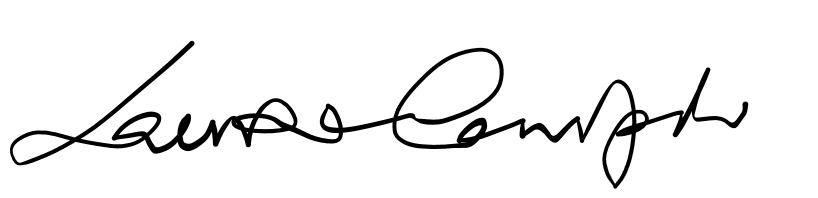
\includegraphics[width=\linewidth]{signature.png} \\
        %\multicolumn{1}{ r| }{}&&&\\
        \multicolumn{1}{ r| }{\textbf{REVIEWED BY:}} & John Cramer & Principal Propulsion Engineer & \\
        %\multicolumn{1}{ r| }{}&&&\\
        \multicolumn{1}{ r| }{\textbf{APPROVED BY:}} & Eleazar Gonzalez-Casas & Chief Engineer & \\
        \hline
    \end{tabular}
\egroup
\end{table}

%\newpage

\begin{abstract}
\noindent Within the framework of the Gilmour Space Technologies Mentorship Program, it was established that, as a first step, one possible direction of work could be the numerical simulation of the gas generator of the Muggera engine which will be tested and adopted by the new liquid rocket engine of Eris. This work aims at reporting all phase of this numerical simulations' campaign.
\end{abstract}

%\newpage

%%%%%%%%%%%%%%%%%%%%%%%%%%%%%%%%%%%%%%%%%%%%%%%%%%%%%%%%%%%%%%%%%%%%%%%
%%%%%%%%%%%%%%%%%%%%%%%%%%%%%%%%%%%%%%%%%%%%%%%%%%%%%%%%%%%%%%%%%%%%%%%
%%%%%%%%%%%%%%%%%%%%%%%%%%%%%%%%%%%%%%%%%%%%%%%%%%%%%%%%%%%%%%%%%%%%%%%

%\pagebreak
%Watermark for rest of document
\AddToShipoutPictureBG{
    \put(0.6\pagewidth,0){
        \transparent{0.3}
\includegraphics[width=7.5cm]{icon.png}%
    }
}
\tableofcontents
%\pagebreak
\listoffigures
\listoftables
%\pagebreak
%Table alternating colours for rest of document
\rowcolors{2}{Table_Dark}{Table_Light}

\section{Introduction}\label{sec:intro}
%%%%%%%%%%%%%%%%%%%%%%%%%%%%%%%%%%%%%%%
A gas generator is a critical component in certain rocket engine designs, particularly those employing a gas-generator cycle. The gas generator is a small combustion chamber within the rocket engine that burns a portion of the propellants to produce hot, high-pressure gas. This gas is not used directly for thrust but instead powers the turbopumps that feed the main combustion chamber with propellants. The gas generator cycle is known for its simplicity and reliability, making it a popular choice for many modern rocket engines.

In particular, the system under investigation runs on non-hypergolic propellant LOX/Jet A-1 in a fuel-rich cycle.
\begin{itemize}
    \item \textbf{LOx (Liquid Oxygen):} LOx is a highly efficient oxidizer with excellent performance characteristics. It is widely available, relatively inexpensive, and can be stored at cryogenic temperatures.
    \item \textbf{Jet-A1:} Jet-A1 is a kerosene-based fuel commonly used in aviation. It has a high energy density, good thermal stability, and low toxicity compared to other rocket fuels like hydrazine. Jet-A1 is less volatile than liquid hydrogen, making it easier and safer to handle.
\end{itemize}

The combination of LOx and Jet-A1 provides a balance of performance, cost-effectiveness, and operational simplicity, making it ideal for gas-generator-cycle engines.

Among key components of the LOx/Jet-A1 gas generator we find:
\begin{itemize}
    \item \textbf{Propellant Injection System:} A small fraction of LOx and Jet-A1 is diverted from the main propellant flow and injected into the gas generator. The injector ensures proper mixing of the oxidizer (LOx) and fuel (Jet-A1) for efficient combustion.
    \item \textbf{Combustion Chamber:} The gas generator has a dedicated combustion chamber where LOx and Jet-A1 are burned. Unlike the main combustion chamber, the gas generator operates at lower pressures and temperatures to avoid damaging downstream components like the turbine.
    \item \textbf{Turbine Drive Gas:} The combustion products from the gas generator are hot gases (primarily $\text{CO}_2$, $\text{H}_2\text{O}$, and some unburned hydrocarbons) that drive the turbine. These gases are typically cooler than those in the main combustion chamber to prevent overheating the turbine blades.
    \item \textbf{Turbopump Assembly:} The turbine converts the thermal energy of the gas into mechanical energy, which drives the fuel and oxidizer pumps. The pumps pressurize the LOx and Jet-A1 before they are fed into the main combustion chamber.
    \item \textbf{Exhaust System:} After driving the turbine, the exhaust gases from the gas generator are either vented overboard or directed into the main nozzle to contribute a small amount of additional thrust.
\end{itemize}

Advantages of the gas generator cycle may include:
\begin{itemize}
    \item \textbf{Simplicity:} The gas generator cycle is mechanically simpler than staged combustion or expander cycles, reducing development time and cost.
    \item \textbf{Reliability:} The lower operating pressures and temperatures in the gas generator reduce thermal and mechanical stresses on components.
    \item \textbf{Reusability:} Engines using the gas generator cycle, such as SpaceX's Merlin engine, have demonstrated reusability, lowering the cost of space launches.
    \item \textbf{Scalability:} The design can be scaled up or down depending on mission requirements.
\end{itemize}

%\newpage

\section{Physical models}
%%%%%%%%%%%%%%%%%%%%%%%%%
The combustion of kerosene can be approximated by the following global reaction:
%
\begin{equation}
    \text{C}_{12}\text{H}_{26} + 18.5\text{O}_2 \rightarrow 12\text{CO}_2 + 13\text{H}_2\text{O}
\end{equation}
%
This reaction represents the complete combustion of dodecane ($\text{C}_{12}\text{H}_{26}$), a common surrogate for kerosene. {Kerosene combustion} involves complex chemical reactions, heat release, and interactions between turbulence and chemistry which demands for appropriate modelling. Options available in OpenFOAM are listed below.
%
%\begin{itemize} % Customize bullet points
%    \item \textbf{Thermophysical Properties}: Density, viscosity, specific heat, thermal conductivity, and latent heat of vaporization.
%    
%    \item \textbf{Chemical Kinetics}: Reaction mechanisms for kerosene combustion (e.g., simplified mechanisms like single-step global reactions or detailed mechanisms).
%    
%    \item \textbf{Combustion Regimes}: Premixed, non-premixed (diffusion), or partially premixed combustion.
%\end{itemize}
%
\begin{table}[H]
\centering
\caption{Typical Physical Properties of Jet A-1.}
\label{tab:jet-fuel-properties}
\begin{tabular}{cc}
\toprule
\textbf{Property} & \textbf{Jet A-1} \\
\midrule
Flash point & $38\,^\circ\mathrm{C}\,(100\,^\circ\mathrm{F})$ \\
Autoignition temperature & $210\,^\circ\mathrm{C}\,(410\,^\circ\mathrm{F})$ \\
Freezing point & $-47\,^\circ\mathrm{C}\,(-53\,^\circ\mathrm{F})$ \\
Max adiabatic burn temperature & $2,230\,^\circ\mathrm{C}\,(4,050\,^\circ\mathrm{F})$ \\
Open air burn temperature & $1,030\,^\circ\mathrm{C}\,(1,890\,^\circ\mathrm{F})$\\
Density at $15\,^\circ\mathrm{C}\,(59\,^\circ\mathrm{F})$ & $0.804\,\mathrm{kg/L}\,(6.71\,\mathrm{lb/US\,gal})$ \\
Specific energy & $43.15\,\mathrm{MJ/kg}\,(11.99\,\mathrm{kWh/kg})$  \\
Energy density & $34.7\,\mathrm{MJ/L}\,(9.6\,\mathrm{kWh/L})$ \\
\bottomrule
\end{tabular}
\end{table}

\begin{itemize}
    \item \textbf{\hl{Breakup model}}
    %%%%%%%%%%%%%%%%%%%%%%%%%%%%%%%%%
    \begin{itemize}
        \item Taylor Analogy Breakup (\textbf{TAB})~\cite{o1987tab}.
        \item Enhanced Taylor Analogy Breakup (\textbf{ETAB})~\cite{tanner1997liquid,tanner1998simulation}.
        \item Secondary Breakup Model (\textbf{SHF})~\cite{schmehl2000cfd} to account for the different breakup regimes, such as bag, multimode, shear.
        \item \textbf{PilchErdman}~\cite{pilch1987use}. Particle secondary breakup model based on the Pilch-Erdman total droplet breakup model.\\
        The droplet fragment velocity is described by the equation:
        \[
            V_d = V \sqrt{\epsilon}(B_1 T + B_2 T^2)
        \]
        where:\\
        
        \begin{tabular}{lp{8cm}}
            $V_d$      & Fragment velocity \\
            $V$        & Magnitude of the relative velocity \\
            $\epsilon$ & Density ratio ($\rho_{\text{carrier}} / \rho_{\text{droplet}}$) \\
            $T$        & Characteristic break-up time \\
            $B_1$      & Model coefficient \\
            $B_2$      & Model coefficient \\
        \end{tabular}\\
        
        The authors suggest the following values for $B_1$ and $B_2$:
        \begin{itemize}
            \item Compressible flow: $B_1 = 0.75 \times 1.0$, $B_2 = 3 \times 0.116$
            \item Incompressible flow: $B_1 = 0.75 \times 0.5$, $B_2 = 3 \times 0.0758$
        \end{itemize}
        \item \textbf{ReitzDiwakar}~\cite{reitz1987modeling,reitz1986effect,reitz1987structure}. Secondary breakup model.
    \end{itemize}
%
    \item \textbf{\hl{Atomization model}}
    %%%%%%%%%%%%%%%%%%%%%%%%%%%%%%%%%%%%%
        \begin{itemize}
            \item \textbf{BlobsSheetAtomization}~\cite{han1997modeling,allocca2002experimental}.%: Primary Breakup Model for pressure swirl atomizers.
            \item \textbf{LISAAtomization}~\cite{senecal1999modeling,schmidt1999pressure}.%: Primary Breakup Model for pressure swirl atomizers.
        \end{itemize}
%
    \item \textbf{\hl{Evaporation model}}%phaseChangeModel
    %%%%%%%%%%%%%%%%%%%%%%%%%%%%%%%%%%%%%
    \begin{itemize}
        \item \textbf{LiquidEvaporation}: Liquid evaporation model using ideal gas assumption.
        \item \textbf{LiquidEvapFuchsKnudsen}~\cite{chen2017numerical}: Liquid evaporation/condensation model for solution of liquid and solid. This model takes into account the Fuchs-Knudsen number correction, the modified Raoult's law is used to obtain the concentration of the evaporable component on the surface, and the activity coefficient is used. The correction Kelvin effect is used.
        \item \textbf{LiquidEvaporationBoil}: Liquid evaporation model using ideal gas assumption and including boiling model based on~\cite{zuo2000studies}.
    \end{itemize}
%
   \item \textbf{\hl{Soot model}}
    %%%%%%%%%%%%%%%%%%%%%%%%%%%%%
    \begin{itemize}
        \item \textbf{grpRadiationSootSubModels}: Liquid evaporation model using ideal gas assumption.
         This soot model is purely a state model. The amount of soot produced is determined by a single-step chemistry as:
        \[
            \nu_f \text{Fuel} + \nu_{\text{Ox}} \text{Ox} = \nu_P P + \nu_{\text{Soot}} \text{Soot}
        \]
        $\nu_{\text{Soot}}$ is prescribed by the user. The single-step chemistry used is read from the combustion. The soot is not considered in the thermodynamics of the system and is not treated as an extra species in the solver.
        
        The spatial distribution is given by the normalization of the first product on the right-hand side (RHS) of the reaction by default, or it can be added as input.
        
        The input dictionary reads as follows in the \texttt{radiationProperties} dictionary:
        \begin{verbatim}
sootModel mixtureFractionSoot<gasHThermoPhysics>;
mixtureFractionSootCoeffs
{
    nuSoot              0.015;
    Wsoot               12;
    mappingField        P;
}
        \end{verbatim}
    \end{itemize}
%
   \item \textbf{\hl{Injection model}}
    %%%%%%%%%%%%%%%%%%%%%%%%%%%%%%%%%%
   \begin{itemize}
        \item \textbf{grpLagrangianIntermediateInjectionSubModels}.
        Injection positions are specified by a particle number density within a cell set.
        The user specifies:
        \begin{itemize}
            \item Number density of particles in the cell set (effective)
            \item Total mass to inject
            \item Initial parcel velocity
        \end{itemize}
        Properties:
        \begin{itemize}
            \item Parcel diameters obtained by a PDF model
            \item All parcels introduced at the start of the simulation (SO)
        \end{itemize}
        \item \textbf{ConeInjection}.
         Multi-point cone injection model.
        The user specifies:
        \begin{itemize}
            \item Time of start of injection
            \item List of injector positions and directions (along injection axes)
            \item Number of parcels to inject per injector
            \item Parcel velocities
            \item Inner and outer half-cone angles
        \end{itemize}
        Properties:
        \begin{itemize}
            \item Parcel diameters obtained by a distribution model
        \end{itemize}
        \item \textbf{ConeNozzleInjection}.
        Cone injection model.
        The user specifies:
        \begin{itemize}
            \item Time of start of injection
            \item Injector position
            \item Direction (along injection axis)
            \item Parcel flow rate
            \item Inner and outer half-cone angles
        \end{itemize}
        Properties:
        \begin{itemize}
            \item Parcel diameters obtained by a size distribution model.
            \item Parcel velocity is calculated as:
                \begin{itemize}
                    \item Constant velocity:
                        \begin{verbatim}
U = <specified by user>
                        \end{verbatim}
                    \item Pressure-driven velocity:
                        \begin{verbatim}
U = sqrt(2*(Pinj - Pamb)/rho)
                        \end{verbatim}
                    \item Flow rate and discharge:
                        \begin{verbatim}
U = V_dot/(A*Cd)
                        \end{verbatim}
                \end{itemize}
        \end{itemize}
        \item \textbf{InflationInjection}. Inflation injection - creates new particles by splitting existing particles within a set of generation cells, then inflating them to a target diameter within the generation cells and an additional set of inflation cells.
        \item \textbf{InjectedParticleDistributionInjection}. Interrogates an \texttt{injectedParticleCloud} to convert the raw particle data into a set of 'binned' injectors.
        The bins are set according to the particle \texttt{tag} property, from which:
        \begin{itemize}
            \item Diameters are converted into \texttt{general distributions} with a user-specified bin width.
            \item Raw velocity and diameter data are resampled and stored to provide variations per injector.
        \end{itemize}
        The mass to inject can be set according to the raw input data mass total by using the \texttt{applyDistributionMassTotal} switch.
        \item \textbf{InjectedParticleInjection}. Replays a set of particle data using the assumption of one particle per parcel based on an \texttt{injectedParticleCloud}.\\
        Example usage in the configuration file:
        \begin{verbatim}
model1
{
    type            injectedParticleInjection;
    SOI             0;
    massTotal       0; // Place holder only
    parcelBasisType fixed;
    nParticle       1; // 1 particle per parcel
    cloud           eulerianParticleCloud;
    positionOffset  (-0.025 2 -0.025);
}
        \end{verbatim}
        \item \textbf{InjectionModel}.
        Templated injection model class.
        The injection model nominally describes the parcel:
        \begin{itemize}
            \item Position
            \item Diameter
            \item Velocity
        \end{itemize}
        In this case, the \texttt{fullyDescribed()} flag should be set to 0 (\texttt{false}). When the parcel is then added to the cloud, the remaining properties are populated using values supplied in the constant properties.
        
        If, however, all of a parcel's properties are described in the model, the \texttt{fullDescribed()} flag should be set to 1 (\texttt{true}).
        \item \textbf{grpLagrangianIntermediateInjectionSubModels}
        Particle injection sources read from a look-up table. Each row corresponds to an injection site.
        \begin{verbatim}
(
    (x y z) (u v w) d rho mDot   // injector 1
    (x y z) (u v w) d rho mDot   // injector 2
    ...
    (x y z) (u v w) d rho mDot   // injector N
);
        \end{verbatim}
        where:\\
        
        \begin{tabular}{lp{8cm}}
            $x, y, z$ & Global Cartesian coordinates [m] \\
            $u, v, w$ & Global Cartesian velocity components [m/s] \\
            $d$       & Diameter [m] \\
            $\rho$    & Density [kg/m$^3$] \\
            $\dot{m}$ & Mass flow rate [kg/s] \\
        \end{tabular}
        \item \textbf{ManualInjection}.
        Manual injection model.
        The user specifies:
        \begin{itemize}
            \item Total mass to inject
            \item Parcel positions in file \texttt{positionsFile}
            \item Initial parcel velocity
        \end{itemize}
        Properties:
        \begin{itemize}
            \item Parcel diameters obtained by a distribution model
            \item All parcels introduced at the start of injection (SOI)
        \end{itemize}
        \item \textbf{PatchFlowRateInjection}.
        Patch injection model, which uses patch flow rate to determine concentration and velocity.
        The user specifies:
        \begin{itemize}
            \item Total mass to inject
            \item Name of patch
            \item Injection duration
            \item Injection target concentration/carrier volume flow rate
        \end{itemize}
        Properties:
        \begin{itemize}
            \item Initial parcel velocity given by local flow velocity
            \item Parcel diameters obtained by a distribution model
            \item Parcels injected randomly across the patch
        \end{itemize}
        \item \textbf{PatchInjection}.
        Patch injection model.
        The user specifies:
        \begin{itemize}
            \item Total mass to inject
            \item Name of patch
            \item Injection duration
            \item Initial parcel velocity
            \item Injection volume flow rate
        \end{itemize}
        Properties:
        \begin{itemize}
            \item Parcel diameters obtained by a distribution model
            \item Parcels injected randomly across the patch
        \end{itemize}
    \end{itemize}
%
    \item{\hl{\textbf{Combustion model}}}
    %%%%%%%%%%%%%%%%%%%%%%%%%%%%%%%%%%%%%
    
    OpenFOAM supports several combustion models depending on the combustion regime, as reported in Table~\ref{tab:combustion-solvers}:
    %
    \begin{itemize}
    \item \textbf{Premixed combustion}: Use the \texttt{XiFoam} solver with flame-wrinkling models.
    \item \textbf{Non-premixed combustion}: Use the \texttt{reactingFoam} solver with PDF-based approaches.
    \item \textbf{Partially premixed combustion}: Use the \texttt{fireFoam} solver for LES simulations.
    \item  \textbf{Partially stirred reactor turbulent combustion model.}  This model calculates a finite rate, based on both turbulence and chemistry time scales. Depending on mesh resolution, the Cmix parameter can be used
    to scale the turbulence mixing time scale.
    \item \textbf{Eddy Dissipation Concept (EDC) turbulent combustion model.}
    This model considers that the reaction occurs in the regions of the flow
    where the dissipation of turbulence kinetic energy takes place (fine
    structures). The mass fraction of the fine structures and the mean residence
    time are provided by an energy cascade model.
%
    There are many versions and developments of the EDC model, 4 of which are
    currently supported in this implementation: v1981, v1996, v2005 and
    v2016.  The model variant is selected using the optional version entry in
    the EDCCoeffs dictionary.
\end{itemize}

% Table 2.1: Combustion solvers in OpenFOAM
\begin{table}[H]
    \centering
    \caption{Combustion solvers in OpenFOAM.}
    \label{tab:combustion-solvers}
    \begin{tabular}{lp{10cm}}
        \toprule
        \textbf{Solver} & \textbf{Description} \\
        \midrule
        sprayFoam & Constant volume combustion solver for compressible flows involving spray parcels. \\
        sprayEngineFoam & Moving piston engine solver for compressible flows involving spray parcels. \\
        coldEngineFoam & Solver for cold flow (without combustion) for internal combustion engines. \\
        engineFoam & Solver for combustion in internal combustion engines. \\
        \bottomrule
    \end{tabular}
\end{table}
%
In~\cite{wang2018physics,xu2018physics}, the \href{https://web.stanford.edu/group/haiwanglab/HyChem}{HyChem} (Hybrid Chemistry) approach to modeling the combustion chemistry of real liquid fuels was developed. The approach takes advantage of the key physics underlying the high-temperature combustion of large hydrocarbon fuels.

\begin{enumerate}
    \item Pyrolysis/oxidative pyrolysis of the fuel occurs first, followed by oxidation of the pyrolysis products.
    \item The oxidation of the pyrolysis products is rate-limiting in the overall fuel oxidation process.
    \item The combustion of the multicomponent fuel follows the principle of large fuel components \cite{xu2019principle}.
\end{enumerate}

The approach combines experimentally constrained, lumped reaction steps for fuel pyrolysis and oxidative pyrolysis with detailed reaction models for the pyrolysis and oxidation of the fuel pyrolysis products. 

For conventional petroleum-derived fuels, the pyrolysis products considered are usually:
\begin{itemize}
    \item Ethylene ($\text{C}_2\text{H}_4$),
    \item Hydrogen ($\text{H}_2$),
    \item Methane ($\text{CH}_4$),
    \item Propene ($\text{C}_3\text{H}_6$),
    \item Iso-butene ($\text{i-C}_4\text{H}_8$),
    \item 1-Butene ($\text{1-C}_4\text{H}_8$),
    \item Benzene ($\text{C}_6\text{H}_6$),
    \item Toluene ($\text{C}_7\text{H}_8$),
    \item Two radical species ($\text{CH}_3$ and $\text{H}$).
\end{itemize}

Other species can be added as needed, depending on the fuel composition. For example, the pyrolysis products of some synthetic fuels can vary with respect to the composition and molecular structure of the parent fuel.


\url{http://combustion.berkeley.edu/gri-mech}
%
    \item \hl{\textbf{Chemical kinetics model}}
    %%%%%%%%%%%%%%%%%%%%%%%%%%%%%%%%%%%%%%%%%%%
    
    Chemical reactions can be modeled using:
    \begin{itemize}
    \item \textbf{Global Mechanisms}: Simplified one-step reactions.
    \item \textbf{Reduced Mechanisms}: Fewer species for computational efficiency.
    \item \textbf{Detailed Mechanisms}: Include hundreds of species for high accuracy.
    \end{itemize}
    Define the reaction mechanism in the \texttt{constant/chemistryProperties} file:
%
\begin{lstlisting}[language={}, caption={Chemistry Properties in OpenFOAM.}]
chemistryReader foamChemistryReader;

foamChemistryFile "$FOAM_CASE/constant/reactions";
foamChemistryThermoFile "$FOAM_CASE/constant/thermo";

solver ode;
\end{lstlisting}

High-speed flow simulations encounter many challenges, such as modeling the high-speed flow-turbulence-chemistry interaction. To simulate these effects accurately, highly refined mesh size as well as \textbf{finite rate chemistry (FRC)} are typically needed, which could easily cause prohibitive computation cost. Even though the low-manifold models such as \textbf{flamelet/progress-variable (FPV)} model is used in some supersonic combustion~\cite{cymbalist2016application}, it is pointed out in~\cite{mrema2019large} that most of these low-manifold models need complicated corrections when applied to fully compressible flows and often mispredict key physical quantities. As a result, \textbf{mechanism reduction} has to be employed for FRC simplifications.

The most commonly seen simplification methodology in combustion simulations is a priori chemical mechanism reduction, such as the methods of \textbf{Direct Relation Graph (DRG)}~\cite{lu2005directed}, \textbf{DRG with Error Propagation (DRGEP)}~\cite{pepiot2008efficient}, \textbf{Path Flux Analysis}~\cite{sun2010path}, and \textbf{Global Pathway Selection (GPS)}~\cite{gao2016global}. The conventional way for mechanism reduction is to
generate the mechanisms under a certain range of operating conditions a priori and subsequently implement these reduced mechanisms into computational fluid dynamics (CFD) combustion simulations. In recent years, the concept of \textbf{dynamic adaptive chemistry (DAC)} scheme which reduces the mechanism on-the-fly at each time step and at each local
computational cell has been extensively studied in reactive flow simulations~\cite{cymbalist2016application,yang2017parallel}. In this way, the number of species could be reduced to smaller values than the conventional calculations, but the on-the-fly mechanism reduction process
itself could incur CPU cost. The tabulated chemistry techniques further reduce the effort of mechanism reduction process as well as the chemistry integration process. Examples of combining DAC and tabulated chemistry can be
found in~\cite{contino2011coupling,yang2017sensitivity,zhou2018computational}.

\textbf{Tabulated dynamic adaptive chemistry (TDAC)}~\cite{contino2011coupling}. is used to accelerate the finite rate chemistry
integration. TDAC is an algorithm that combines in situ adaptive tabulation (ISAT)~\cite{pope1997computationally} and dynamic adaptive chemistry (DAC)~\cite{liang2009dynamic}. In conventional DAC, the mechanism reduction process is conducted at each time step and each grid point to generate an optimal reduced mechanism considering the local and current thermodynamic conditions and species composition. However, the mechanism reduction process could incur expensive computation, especially with large amount of grid points. In TDAC, this issue is addressed by the ISAT technique, which only requires mechanism reduction when the current and local state is not within the accuracy region of the tabulated chemistry. In ISAT, this accuracy region is quantified and the tabulation is dynamically increased. Another important feature of TDAC is the reduction on species transport equations. When reduced mechanism is produced and unimportant species are eliminated, only the important species transport equations are solved, which further significantly reduce the computational cost.

%
    \item \hl{\textbf{Thermophysical model}}
    %%%%%%%%%%%%%%%%%%%%%%%%%%%%%%%%%%%%%%%%
    
    OpenFOAM requires thermophysical properties for kerosene (e.g., Jet A/A-1) to be defined in the \texttt{constant/thermophysicalProperties} file. Surrogate fuels like n-decane or n-dodecane are often used to approximate kerosene properties.
    %
\begin{lstlisting}[language={bash}, caption={Thermophysical Properties in OpenFOAM.}]
thermoType
{
    type            hePsiThermo;
    mixture         pureMixture;
    transport       const;
    thermo          hConst;
    equationOfState perfectGas;
    specie          specie;
    energy          sensibleEnthalpy;
}

mixture
{
    specie
    {
        molWeight       142; // Approximate molecular weight of kerosene
    }
    thermodynamics
    {
        Cp              2000; // Specific heat capacity [J/kg/K]
        Hf              -5000000; // Heat of formation [J/kg]
    }
    transport
    {
        mu              1e-5; // Dynamic viscosity [Pa.s]
        Pr              0.7; // Prandtl number
    }
}
\end{lstlisting}

\begin{lstlisting}[language=C++, caption={OpenFOAM Sub-Models Configuration}]
subModels
{
    particleForces
    {
        sphereDrag;
    }
    injectionModels
    {
        model1
        {
            type            coneNozzleInjection;
            SOI             0;
            parcelBasisType mass;
            injectionMethod disc;
            flowType        flowRateAndDischarge;
            position        (0 0 0);
            direction       (1 0 0);
            parcelsPerSecond 700000000; // (Di Ilio et al., (2019), p. 6)
            #include "<constant>/massFlowRateProfile.foam"
            thetaInner      constant 0.0;
            thetaOuter      constant 11.0; // (Di Ilio et al., (2019), p. 4)
            sizeDistribution
            {
                type        RosinRammler;
                RosinRammlerDistribution
                {
                    minValue        1e-06;
                    maxValue        18e-06;
                    d               6e-06;
                    n               3;
                }
            }
        }
    }
    dispersionModel stochasticDispersionRAS;
    patchInteractionModel none;
    heatTransferModel RanzMarshall;
    compositionModel singlePhaseMixture;
    phaseChangeModel liquidEvaporationBoil;
    surfaceFilmModel none;
    atomizationModel none;
    breakupModel ReitzKHRT;
    stochasticCollisionModel none;
    radiation       off;
    RanzMarshallCoeffs
    {
        BirdCorrection  true;
    }
    singlePhaseMixtureCoeffs
    {
        phases
        (
            liquid
            {
                C12H26    1;
            }
        );
    }
    liquidEvaporationBoilCoeffs
    {
        enthalpyTransfer enthalpyDifference;
        activeLiquids    ( C12H26 );
    }
    ETABCoeffs
    {
        // (Wehrfritz et al. (2013), Table 2)
        Cmu             10.0;
        Comega          8.0;
        WeCrit          12;
        k1              0.2;
        k2              0.2;
        WeTransition    100.0;
    }
    ReitzKHRTCoeffs
    {
        defaultCoeffs   no;
        B0              0.61;
        B1              18;
        Ctau            1.0;
        CRT             0.1;
        msLimit         0.3;
        WeberLimit      6.0;
        // (Wehrfritz et al. (2013), Table 1)
     /* defaultCoeffs   no;
        B0              0.61;
        B1              40;
        Ctau            1.0;
        CRT             0.1;
        msLimit         0.03;
        WeberLimit      6.0; */
    }
}
\end{lstlisting}
\item \textbf{\hl{particleForces}}
\item \textbf{\hl{dispersionModel}}
\item \textbf{\hl{patchInteractionModel}}
\item \textbf{\hl{heatTransferModel}}: RanzMarshall
\item \textbf{\hl{compositionModel}} singlePhaseMixture
%\item phaseChangeModel liquidEvaporationBoil 
\item \textbf{\hl{surfaceFilmModel}}
%\item atomizationModel 
%\item breakupModel ReitzKHRT 
\item \textbf{\hl{stochasticCollisionModel}}
\item \textbf{\hl{radiation}}
\end{itemize}

% https://www.openfoam.com/documentation/guides/v1912/api/classFoam_1_1SinglePhaseMixture.html#details
%\subsection*{Lagrangian Solvers}
%\begin{itemize}
%    \item coalChemistryFoam.C
%    \item DPMFoam.C
%    \item MPPICFoam.C
%    \item icoUncoupledKinematicParcelDyMFoam.C
%    \item icoUncoupledKinematicParcelFoam.C
%    \item reactingHeterogenousParcelFoam.C
%    \item reactingParcelFoam.C
%    \item simpleCoalParcelFoam.C
%    \item simpleSprayFoam.C
%    \item sprayDyMFoam.C
%    \item sprayFoam.C
%    \item uncoupledKinematicParcelFoam.C
%\end{itemize}
%
%\subsection*{Lagrangian Particle Models}
%\begin{itemize}
%    \item Clouds
%    \item Parcels
%    \item Submodels
%    \begin{itemize}
%        \item Function objects
%        \begin{itemize}
%            \item CloudFunctionObject
%            \item FacePostProcessing
%            \item ParticleCollector
%            \item ParticleErosion
%            \item ParticleTracks
%            \item ParticleTrap
%            \item PatchPostProcessing
%            \begin{itemize}
%                \item VoidFraction
%            \end{itemize}
%        \end{itemize}
%    \end{itemize}
%
%    \item Kinematic
%    \begin{itemize}
%        \item Collision
%        \item Dispersion
%        \item Forces
%        \item Injection
%        \item Patch interaction
%        \begin{itemize}
%            \item Surface film
%        \end{itemize}
%        \item MP-PIC
%    \end{itemize}
%
%    \item Reacting
%    \begin{itemize}
%        \item Atomization
%        \begin{itemize}
%            \item AtomizationModel
%            \begin{itemize}
%                \item BlobsSheetAtomization
%                \item LISAAtomization
%                \item NoAtomization
%            \end{itemize}
%        \end{itemize}
%
%        \item Breakup
%        \begin{itemize}
%            \item BreakupModel
%            \begin{itemize}
%                \item ETAB
%                \item NoBreakup
%                \item PilchErdman
%                \item ReitzDiwakar
%                \item ReitzKHRT
%                \item SHF
%                \item TAB
%            \end{itemize}
%        \end{itemize}
%
%        \item Composition
%        \begin{itemize}
%            \item CompositionModel
%            \begin{itemize}
%                \item NoComposition
%                \item SingleMixtureFraction
%                %\begin{itemize}
%                %    \item SinglePhaseMixture
%                %\end{itemize}
%            \end{itemize}
%        \end{itemize}
%
%        \item Phase change
%        \begin{itemize}
%            \item LiquidEvaporation
%            \item LiquidEvaporationBoil
%            \item NoPhaseChange
%            \begin{itemize}
%                \item PhaseChangeModel
%            \end{itemize}
%        \end{itemize}
%
%        \item Reacting multiphase
%        \begin{itemize}
%            \item Devolatilisation
%            \item Surface reaction
%        \end{itemize}
%
%        \item Thermodynamic
%
%        \item Heat transfer
%        \begin{itemize}
%            \item HeatTransferModel
%            \begin{itemize}
%                \item NoHeatTransfer
%                \item RanzMarshall
%            \end{itemize}
%        \end{itemize}
%    \end{itemize}
%\end{itemize}
%
%\subsection*{Combustion Models}
%\begin{itemize}
%    %\item combustionModel
%    \item diffusion
%    \item diffusionMulticomponent
%    \item eddyDissipationDiffusionModel
%    \item Flame Surface Dennsity (FDS)
%    \item infinitelyFastChemistry
%    \item laminar
%    \item noCombustion
%    \item PaSR
%    \item singleStepCombustion
%\end{itemize}
%
%\subsection*{Turbulence Models}
%\begin{itemize}
%    \item Turbulence Models
%    \begin{itemize}
%        \item Boundary conditions
%        \item Compressible turbulence
%        \item DES turbulence
%        \item Incompressible turbulence
%        \item LES turbulence
%        \item RAS turbulence
%        \item Laminar transport model
%    \end{itemize}
%
%    \item Turbulence Modeling Approaches
%    \begin{itemize}
%        \item Eddy viscosity
%        \item Linear viscous stress
%        \item Nonlinear eddy viscosity
%        \item Reynolds stress
%        \item General turbulence model
%    \end{itemize}
%\end{itemize}

\section{Numerical approach}\label{sec"sim}
%%%%%%%%%%%%%%%%%%%%%%%%%%%%%%%%%%%%%%%%%%%%
%OpenFOAM provides tools to simulate these processes using various solvers and combustion models. 
This document outlines the steps to characterize kerosene combustion in \textbf{OpenFOAM} and \textbf{Fluent}, including thermophysical property definitions, solver selection, and workflow.

\subsection{OpenFOAM}\label{secsubsec:OF}
%%%%%%%%%%%%%%%%%%%%%%%%%%%%%%%%%%%%%%%%%

\subsubsection*{Solver selection}
%%%%%%%%%%%%%%%%%%%%%%%%%%%%%%%%%
Below is a summary of various OpenFOAM solvers and their descriptions:

\begin{table}[H]
\centering
\caption{OpenFOAM Solvers for Combustion and Related Problems}
\label{tab:openfoam-solvers}
\begin{tabular}{lp{10cm}}
\toprule
\textbf{Solver Name} & \textbf{Description} \\
\midrule
\texttt{chemFoam} & Solver for chemistry problems, designed for use on single-cell cases to provide comparison against other chemistry solvers. Uses a single-cell mesh and fields created from initial conditions. \\
\texttt{coldEngineFoam} & Solver for cold-flow in internal combustion engines. \\
\texttt{fireFoam} & Transient solver for fires and turbulent diffusion flames with reacting particle clouds, surface film, and pyrolysis modeling. \\
\texttt{PDRFoam} & Solver for compressible premixed/partially-premixed combustion with turbulence modeling. \\
\texttt{reactingFoam} & Solver for combustion with chemical reactions. \\
\texttt{rhoReactingBuoyantFoam} & Solver for combustion with chemical reactions using a density-based thermodynamics package with enhanced buoyancy treatment. \\
\texttt{rhoReactingFoam} & Solver for combustion with chemical reactions using a density-based thermodynamics package. \\
\texttt{XiFoam} & Solver for compressible premixed/partially-premixed combustion with turbulence modeling. \\
\texttt{XiDyMFoam} & Solver for compressible premixed/partially-premixed combustion with turbulence modeling. \\
\texttt{XiEngineFoam} & Solver for internal combustion engines. \\
\bottomrule
\end{tabular}
\end{table}

\begin{table}[H]
\centering
\caption{Comparison of OpenFOAM Solvers for Compressible Flow Simulations}
\label{tab:openfoam_solvers}
\adjustbox{max width=\textwidth}{%
\begin{tabular}{lccccc}
\hline
\textbf{Solver} & \textbf{Type} & \textbf{Turbulence} & \textbf{Compressible} & \textbf{Combustion/Reactivity} & \textbf{Algorithm} \\
\hline
rhoSimpleFoam & Steady-state & Yes & Yes & No & SIMPLE \\
rhoPimpleFoam & Transient & Yes & Yes & No & PIMPLE (PISO-SIMPLE) \\
rhoCentralFoam & Transient & Optional & Yes & No & Central-differencing (shock-resolving) \\
rhoReactingFoam & Transient & Yes & Yes & Yes & PISO/SIMPLE \\
\hline
\end{tabular}}
\end{table}

\subsubsection*{Mesh generation}
%%%%%%%%%%%%%%%%%%%%%%%%%%%%%%%%
The mesh generation process in OpenFOAM relies on tools like \texttt{blockMesh}, \texttt{snappyHexMesh} or  \texttt{cfMesh}.

\subsubsection*{Initial conditions}
%%%%%%%%%%%%%%%%%%%%%%%%%%%%%%%%%%%

\subsubsection*{Boundary conditions}
%%%%%%%%%%%%%%%%%%%%%%%%%%%%%%%%%%%%
The \textbf{fixedFluxPressure} is a pressure boundary condition to set the pressure gradient to the provided value such that the flux on the boundary is that specified by the velocity boundary condition. This condition ensures the correct flux at fixed-flux boundaries by compensating for the body forces (gravity in particular) with the pressure gradient.

The \textbf{waveTransmissive} is a general boundary condition that provides a wave transmissive outflow condition, based on solving DDt(W, field) = 0 at the boundary, W is the wave velocity and field is the field to which this boundary condition is applied.

The \textbf{totalPressure} is a boundary condition that sets the static pressure at the patch based on a specification of the total pressure, . The mode of operation is determined via the input entries and the dimensions of the convective flux, phi ().

Define boundary conditions in the \texttt{0/U} file:

\begin{lstlisting}[language={}, caption={Boundary Conditions in OpenFOAM}]
boundaryField
{
    inlet
    {
        type            fixedValue;
        value           uniform (10 0 0); // Velocity vector
    }
    outlet
    {
        type            zeroGradient;
    }
    walls
    {
        type            noSlip;
    }
}
\end{lstlisting}

\subsubsection*{Post-Processing}
%%%%%%%%%%%%%%%%%%%%%%%%%%%%%%%%
Use OpenFOAM utilities and ParaView for post-processing:

\begin{itemize}
    \item Visualize temperature, species concentrations, and velocity fields.
    \item Analyze flame structure, ignition delay, and pollutant formation (e.g., NOx, CO).
\end{itemize}

\subsection{Fluent}\label{subsec:Fluent}
%%%%%%%%%%%%%%%%%%%%%%%%%%%%%%%%%%%%%%%%
% https://www.afs.enea.it/project/neptunius/docs/fluent/html/ug/node520.htm
% https://www.afs.enea.it/project/neptunius/docs/fluent/html/ug/node1036.htm#Species_Model

\subsubsection{Stability and Convergence in Reacting Flows}
%%%%%%%%%%%%%%%%%%%%%%%%%%%%%%%%%%%%%%%%%%%%%%%%%%%%%%%%%%%
Obtaining a converged solution in a reacting flow can be difficult for a number of reasons. First, the impact of the chemical reaction on the basic flow pattern may be strong, leading to a model in which there is strong coupling between the mass/momentum balances and the species transport equations. This is especially true in combustion, where the reactions lead to a large heat release and subsequent density changes and large accelerations in the flow. All reacting systems have some degree of coupling, however, when the flow properties depend on the species concentrations. These coupling issues are best addressed by the use of a two-step solution process and by the use of under-relaxation.

A second convergence issue in reacting flows involves the magnitude of the reaction source term. When the ANSYS FLUENT model involves very rapid reaction rates (reaction time scales are much faster than convection and diffusion time scales), the solution of the species transport equations becomes numerically difficult. Such systems are termed "stiff'' systems. Stiff systems with laminar chemistry can be solved using either the pressure-based solver with the Stiff Chemistry Solver option enabled, or the density-based solver. The laminar chemistry model may also be used for turbulent flames, where turbulence-chemistry interactions are neglected. However, for such flames, the Eddy-Dissipation Concept or PDF Transport models, which account for turbulence-chemistry interactions, may be a better choice. 

\subsubsection{Ignition in Combustion Simulations}
%%%%%%%%%%%%%%%%%%%%%%%%%%%%%%%%%%%%%%%%%%%%%%%%%%
% https://www.afs.enea.it/project/neptunius/docs/fluent/html/ug/node801.htm#sec-patch
If you introduce fuel to an oxidant, spontaneous ignition does not occur unless the temperature of the mixture exceeds the activation energy threshold required to maintain combustion. This physical issue manifests itself in an ANSYS FLUENT simulation as well. If you are using the laminar finite-rate, finite-rate/eddy-dissipation, Eddy-Dissipation Concept or PDF Transport model for turbulence-chemistry interaction, you have to supply an ignition source to initiate combustion. This ignition source may be a heated surface or inlet mass flow that heats the gas mixture above the required ignition temperature. Often, however, it is the equivalent of a spark: an initial solution state that causes combustion to proceed. You can supply this initial spark by patching a hot temperature into a region of the ANSYS FLUENT model that contains a sufficient fuel/air mixture for ignition to occur. 

\section{Testcases}\label{sec:testcase}
%%%%%%%%%%%%%%%%%%%%%%%%%%%%%%%%%%%%%%%
The Muggera gas generator will be numerically simulated by comparing solutions from OpenFOAM and Fluent solvers.

%%%%%%%%%%%%%%%%%%%%%%%%%%%%%%%%%%%%%%%%%%
\subsection{Muggera}\label{subsec:muggera}
%%%%%%%%%%%%%%%%%%%%%%%%%%%%%%%%%%%%%%%%%%
%\subsection{Uni-element rocket injector}
%%%%%%%%%%%%%%%%%%%%%%%%%%%%%%%%%%%%%%%%

\begin{figure}[H]
    \centering
    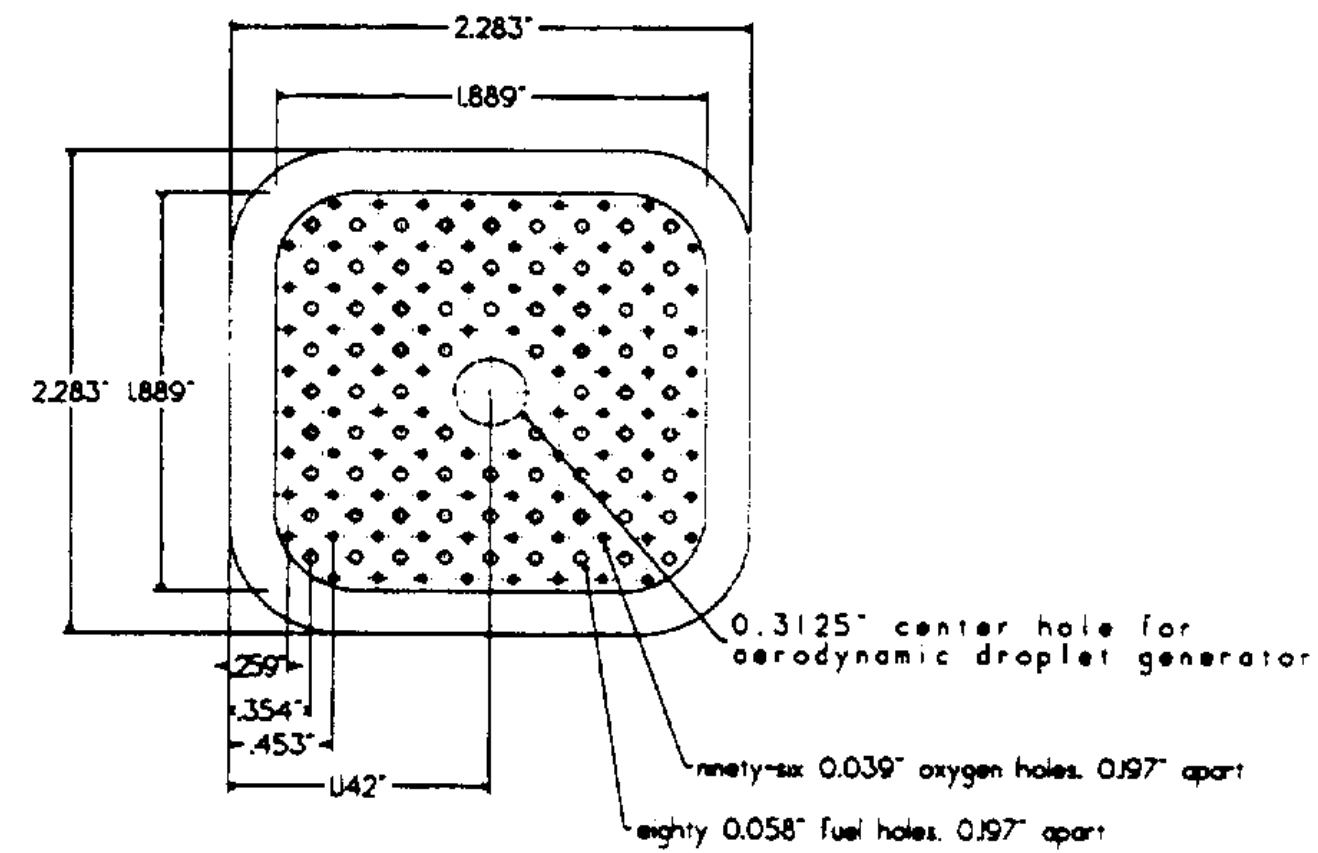
\includegraphics[width=0.35\linewidth]{figs/CCL/fig0.png}
    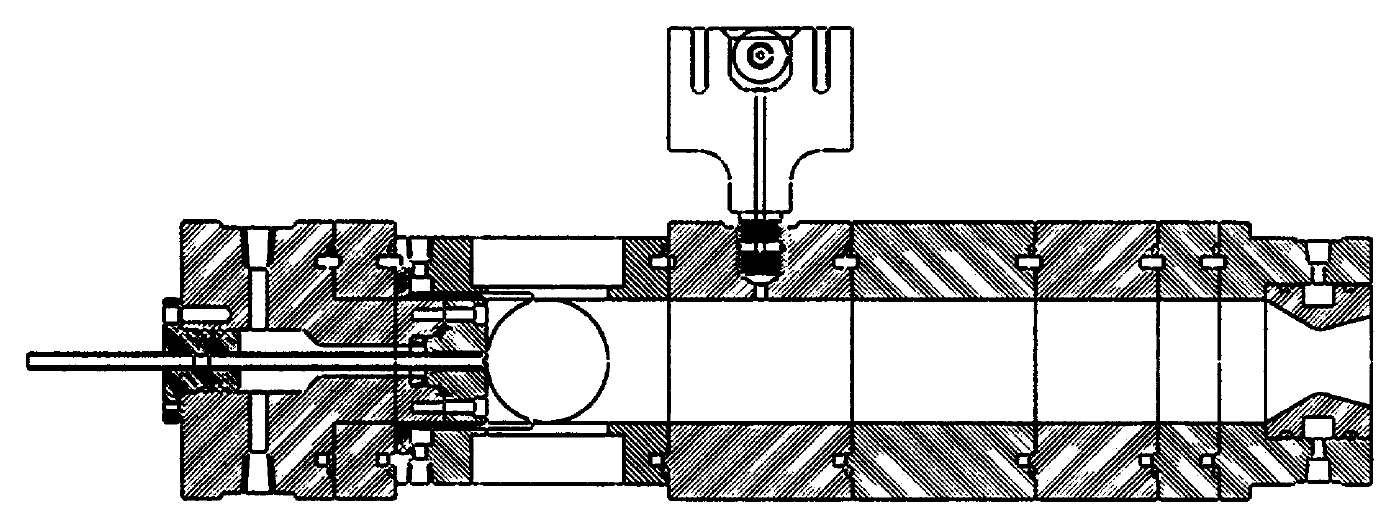
\includegraphics[width=0.5\linewidth]{figs/CCL/fig2a.png}
    \caption{Schematic of the optically-accessible rocket chamber. The chamber is designed such that optical access can be gained for any axial location by interchanging sections. From~\cite{santoro1997experimental, santoro1999main}.}
    \label{fig:enter-label}
\end{figure}

\begin{figure}[H]
    \centering
    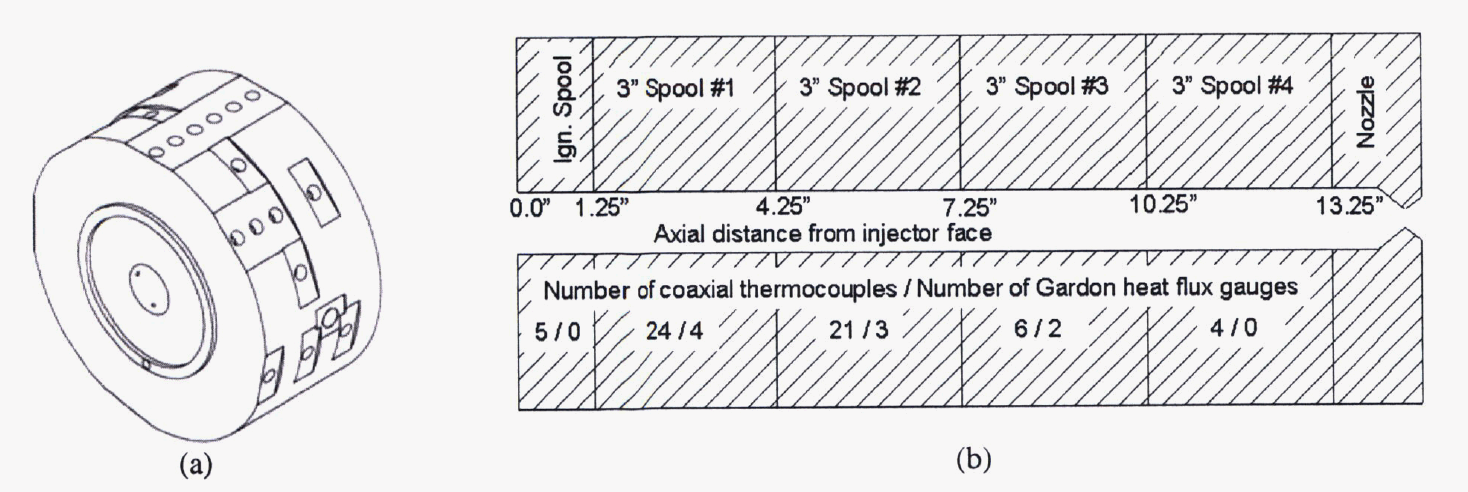
\includegraphics[width=\linewidth]{figs/CCL/fig4.png}
    \caption{(a) Isometric view of combustion chamber spool piece, showing typical locations for instrumentation. (b) Combustion chamber cross section, listing typical instrumentation in each spool piece. From~\cite{jones2006local}.}
    \label{fig:enter-label}
\end{figure}

\begin{figure}[H]
    \centering
    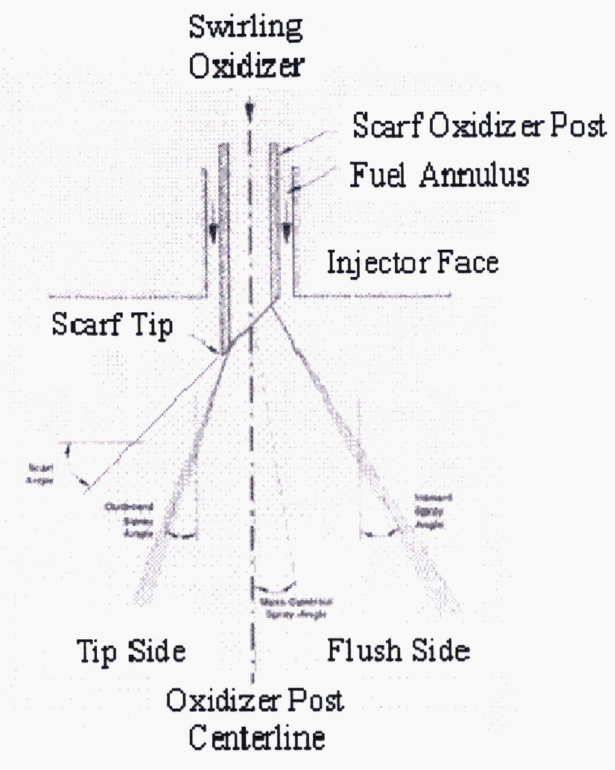
\includegraphics[width=\linewidth]{figs/CCL/fig14.png}
    \caption{Scarf swirl element nomenclature. From~\cite{jones2006local}.}
    \label{fig:enter-label}
\end{figure}

%\subsection{SandiaD\_LTS}
%%%%%%%%%%%%%%%%%%%%%%%%%
The \textbf{SandiaD\_LTS} is based on experimental data from Sandia National Laboratories, specifically focusing on turbulent flame dynamics in combustion systems. The turbulent non-premixed Sandia Flame D, studied experimentally by Barlow and Frank~\cite{barlow2005piloted}, is of particular interest as a large amount of data is available for temperature, major species, and pollutant concentrations in the flame and post-flame regions. This configuration was extensively used as a validation case for pollutant formation modelling, as it contains some essential features of turbulence/chemistry interaction

Although the density-based solver developed in this study is fully-compressible, we will show in this section that it is still able to well capture the flow and flame field at Ma = 0.1 − 0.2. The Sandia Flame D piloted partially premixed flame (the maximum Mach number in this flame is about 0.17) is simulated with the TDAC method. Sandia Flame D documentation provides detailed experimental data and the flames are widely validated with different CFD frameworks. Fully compressible solvers is firstly used for Sandia Flame D by Yang et al. with preconditioning scheme. The flow conditions in Sandia Flame D is presented in Table 1. In this study, the current solver is used for the low-speed Sandia Flame D with purpose of testifying the capability of our solve in the low Mach number range. A 2D wedge computational domain is used in this simulation with the Reynolds Averaged transport equations. The Reynolds stress term is closed with the \textbf{standard k − $\epsilon$ model}. Turbulence-chemistry interaction is handles by the \textbf{EDC model}. The chemistry source term integration is achieved
by solving a series of ODE equations, where \textbf{tabulated dynamic adaptive chemistry (TDAC)} is used to accelerate the computation. \textbf{GRI3.0 mechanism} [31] is used for the chemical kinetics.

\subsubsection*{Computational domain and numerical setup}
Present investigation case is Sandia Flame D~\cite{barlow2005piloted} and the burner schematic is shown in Fig.~\ref{fig:domain}. The axisymmetric piloted burner has a main jet inner diameter (D) of 7.2 mm. The pilot annulus inner diameter and outer diameter is 7.7 mm and 18.2 mm, respectively. The burner outer wall diameter is 18.9 mm. Computational domain is a wedge with 5° and its axial and radial length is 80D × 20D. Grid cells around the axis and has a resolution of 162 × 1 × 500. The mesh has a minimum grid of 0.125 mm and a total cell number of 81000. Based on Reynolds numbers of 22 400, air-coow, piloted jet and main fuel jet have bulk inflow velocity of 0.9 m s−1, 11.4 m s−1 and 49.6 m s−1 , and have inflow temperature of 291 K, 1880 K and 294 K, respectively. The velocities of coflow and main fuel jet are under the standard state of 294 K, 0.993 atm. The pilot bulk velocity is estimated from the specified conditions, the flow area of the pilot annulus and the measured mass flow rates. The ambient pressure is 0.996 atm. Fuel is $CH_4$/air mixtures with a volume ratio of 1:3 $\delta$Z ¼ 1. The piloted jet is burned mixtures containing $C_2H_2$, $H_2$, air, $CO_2$ and $N_2$ Z ¼ 0:271. The pressure inlet boundary condition adopts the Neumann condition, and the pressure outlet boundary condition adopts the Dirichlet condition. The inlet boundary condition of other solution variables adopts Dirichlet condition, the outlet boundary condition adopts Neumann condition, and the wall adopts noslip wall condition. Specifically, the $k$ and $\omega$ use the wall function. Periodic boundary conditions are used on the left and right sides.

\begin{figure}[H]
    \centering
    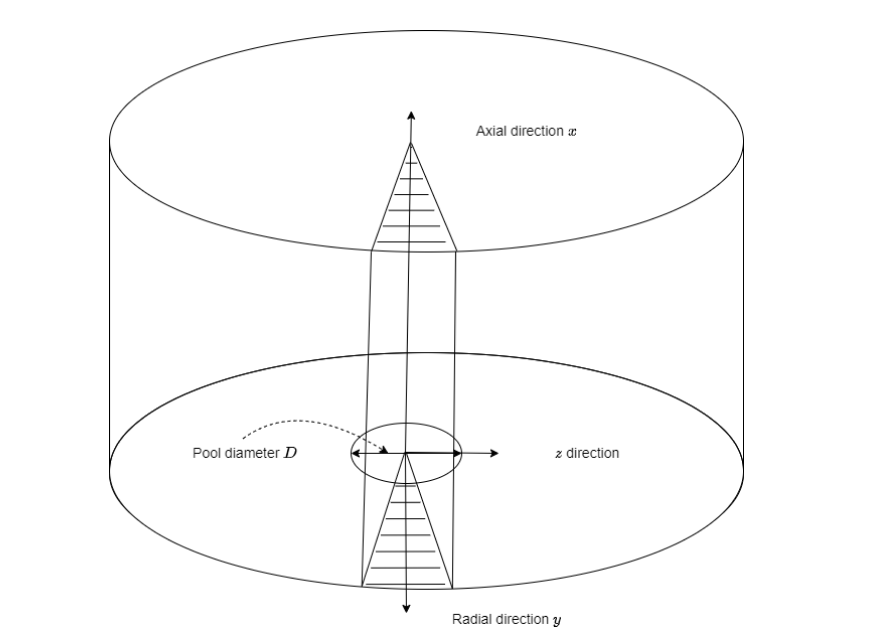
\includegraphics[width=0.95\linewidth]{figs/SandiaD/Screenshot from 2025-03-12 08-14-12.png}
    %\caption{Schematic representation of the numeric domain in the SandiaD LTS tutorial case. Dimensions in mm.}
    \label{fig:domain2}
\end{figure}

\begin{figure}[H]
    \centering
    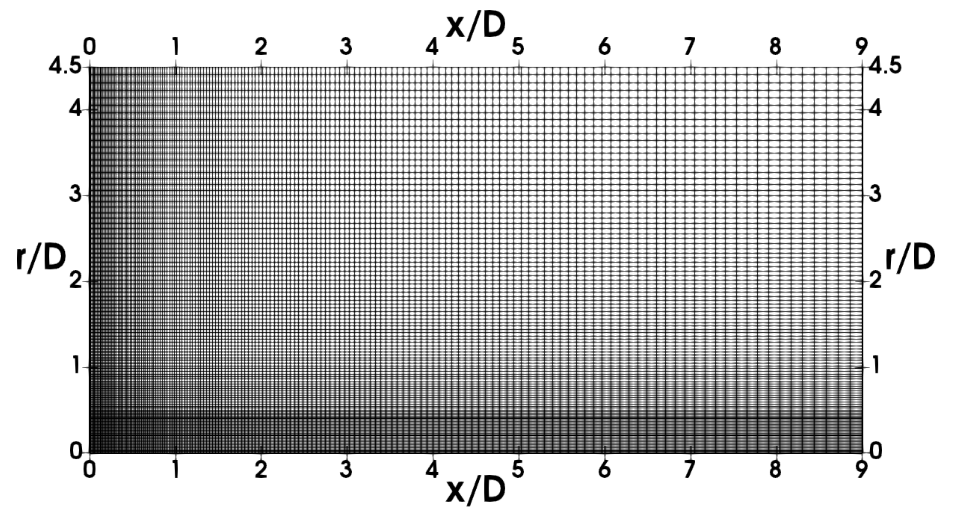
\includegraphics[width=0.95\linewidth]{figs/SandiaD/Screenshot from 2025-03-12 08-14-26.png}
    %\caption{Schematic representation of the numeric domain in the SandiaD LTS tutorial case. Dimensions in mm.}
    \label{fig:domain2}
\end{figure}

\begin{figure}[H]
    \centering
    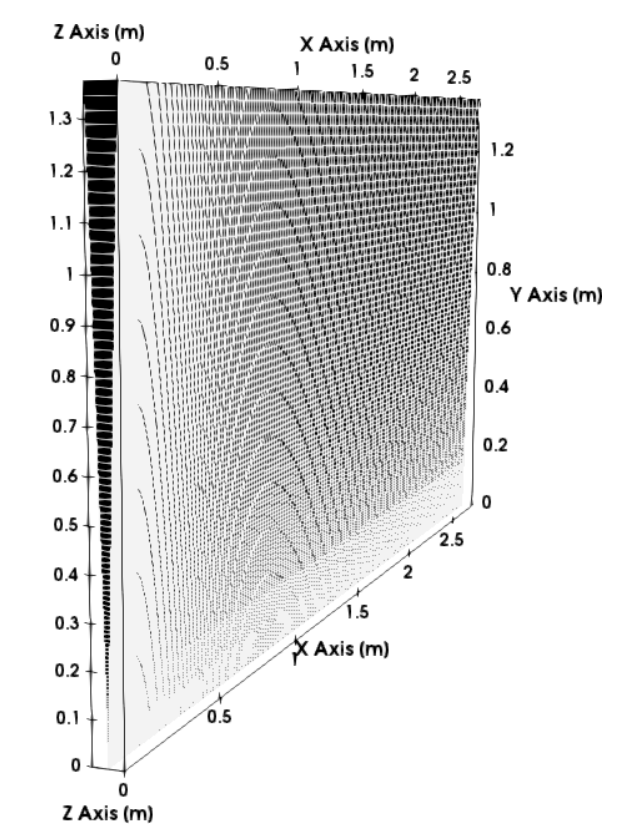
\includegraphics[width=0.65\linewidth]{figs/SandiaD/Screenshot from 2025-03-12 08-15-01.png}
    %\caption{Schematic representation of the numeric domain in the SandiaD LTS tutorial case. Dimensions in mm.}
    \label{fig:domain2}
\end{figure}

\begin{figure}[H]
    \centering
    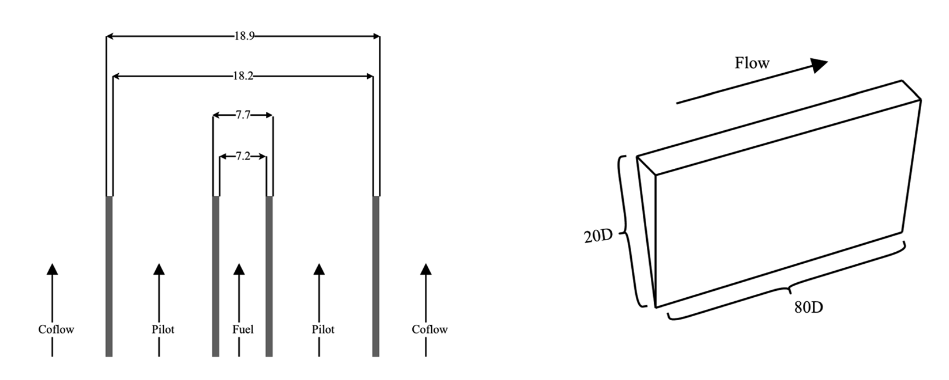
\includegraphics[width=0.95\linewidth]{figs/SandiaD/Screenshot from 2025-03-12 07-11-47.png}
    \caption{The burner schematic in cross section view (a) and axis view (b) of the Sandia Flame D.}
    \label{fig:domain}
\end{figure}

\begin{figure}[H]
    \centering
    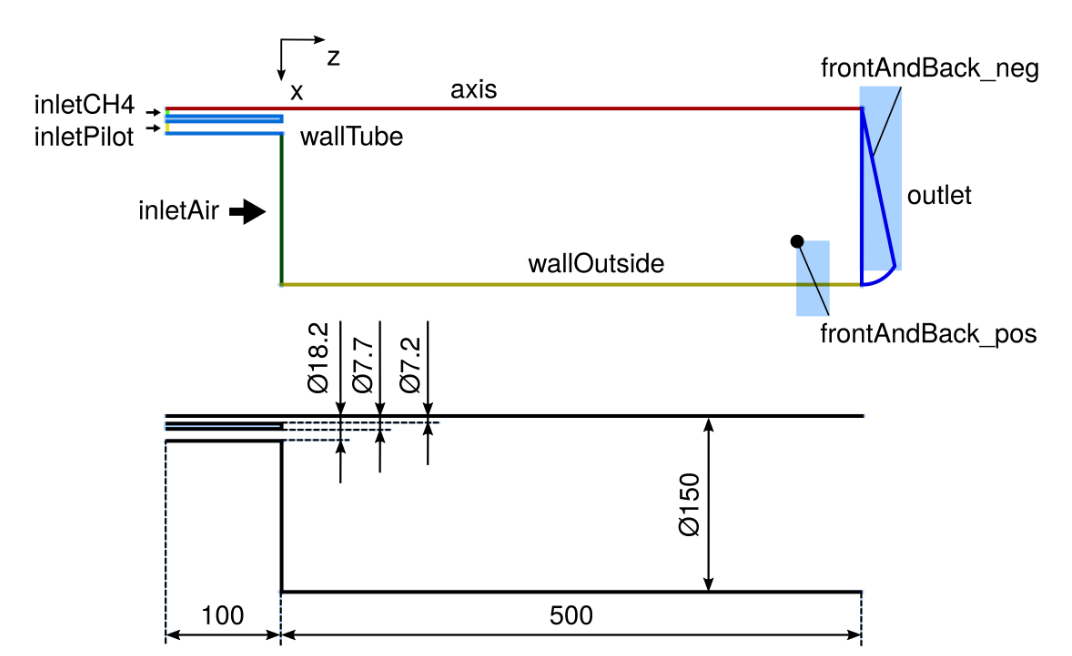
\includegraphics[width=0.95\linewidth]{figs/SandiaD/Screenshot from 2025-03-12 06-58-20.png}
    \caption{Schematic representation of the numeric domain in the SandiaD LTS tutorial case. Dimensions in mm.}
    \label{fig:domain2}
\end{figure}

\subsubsection*{Initial and boundary conditions (0)}
The 0 directory contains pressure $p$, velocity $U$, turbulence kinetic energy $k$, turbulence dissipation rate $\omega$, turbulence viscosity $\nu_t$, and turbulent thermal diffusivity $\alpha_t$. Also, temperature $T$ and incident radiation $G$, as well as the mass fractions of $CO$, $CO_2$, $H$, $H_2$, $H_2O$, $N_2$, $O$, $O_2$ and $OH$. The initial and boundary conditions for the mass fractions of all other included species are set by $Y$default. The computational domain is a wedge representing the axisymmetric setup. The boundaries and dimensions of the domain are shown in Figure~\ref{fig:domain2}. A rich methane-air mixture with 25\% $CH_4$ enters the domain at inletCH4, corresponding to a fuel-air equivalence ratio $\phi$ = 3.17. The diameter of inletCH4 is 7.2 mm. Both inletCH4 and inletPilot are modelled from 100 mm upstream of the expansion to wallOutside. An overview over selected inlet boundary conditions is given in Table~\ref{tab:inlet_boundaries}.

\begin{table}[H]
\centering
\caption{Inner and outer diameter in mm, axial velocity component in m/s, turbulence intensity, mixing length in m, temperature in K, and equivalence ratio at the three inlet boundaries.}
\label{tab:inlet_boundaries}
\adjustbox{max width=\textwidth}{%
\begin{tabular}{cccccccc}
\hline
\textbf{Inlet} & \textbf{$d_i$ (mm)} & \textbf{$D$ (mm)} & \textbf{$U$ (m/s)} & \textbf{Turb. Intensity} & \textbf{Mix. Length (m)} & \textbf{$T$ (K)} & \textbf{$\phi$} \\ \hline
inletCH4       & -                   & 7.2               & 49.6               & 0.0458                  & $5.04 \times 10^{-4}$   & 294              & 3.17            \\ \hline
inletPilot     & 7.7                 & 18.2              & 11.4               & 0.0628                  & $7.35 \times 10^{-4}$   & 1880             & 0.77            \\ \hline
inletAir       & 18.2                & 300               & 0.9                & 0.0471                  & 0.019677                 & 291              & 0               \\ \hline
\end{tabular}}
\end{table}

The lean combustion process of the pilot flame is not solved, instead an inlet condition corresponding the product of the combustion process is prescribed at inletPilot. The inlet temperature at the pilot inlet is set to 1880 K, and the product concentration was calculated separately for a premixed unstrained flame at $\phi$ = 0.77, with the mass fractions of the major species and radicals given in Table~\ref{tab:species_mass_fractions}. At inletAir, air at a temperature of 291 K enters the domain at a speed of 0.9 m/s.

\begin{table}[H]
\centering
\caption{Species mass fractions at the three inlet boundaries.}
\label{tab:species_mass_fractions}
\adjustbox{max width=\textwidth}{%
\begin{tabular}{ccccccccccc}
\hline
\textbf{Inlet} & \textbf{N2} & \textbf{O2} & \textbf{CH4} & \textbf{CO2} & \textbf{H2O} & \textbf{H2} & \textbf{OH} & \textbf{CO} & \textbf{O} & \textbf{H} \\ \hline
inletCH4       & 0.6473      & 0.1966      & 0.1561       & 0            & 0            & 0           & 0           & 0          & 0         & 0        \\ \hline
inletPilot     & 0.7342      & 0.054       & 0            & 0.1098       & 0.0942       & $1.29 \times 10^{-4}$ & $2.8 \times 10^{-3}$ & $4.07 \times 10^{-3}$ & $7.47 \times 10^{-4}$ & $2.48 \times 10^{-5}$ \\ \hline
inletAir       & 0.77        & 0.23        & 0            & 0            & 0            & 0           & 0           & 0          & 0         & 0        \\ \hline
\end{tabular}}
\end{table}

A no-slip condition is specified at wallTube, while zero velocity gradient is specified at wallOutside. Wall functions are applied for both wall patches for $k$, $\omega$ and $nu_t$. The outlet is modelled as a 1e5 Pa total pressure outlet.

\subsubsection*{chemistryProperties.orig}
Under \hl{\texttt{chemistryType}}, the solver \texttt{ode} is selected to solve ordinary differential equations. Tabulation of Dynamic Adaptive Chemistry (TDAC) is chosen as the solution method to speed up chemistry calculations. This feature was added in OpenFOAM-v5. It was demonstrated that this chemistry reduction can increase the efficiency of solving species transport in the case of modestly detailed reaction mechanisms like GRI-Mech 3.0~\cite{ref6}. The initial chemical time step size is set to $1 \times 10^{-7}$ s, which is independent of the flow time step size specified in \texttt{system/controlDict}. 

Under \texttt{odeCoeffs}, the ODE solver \texttt{seulex} is selected, and absolute and relative tolerances are specified. Under \texttt{importantSpecies}, the species which are to be left together with elementary reactions at the end of the reduction process are specified~\cite{ref7}. Finally, the tolerances for reduction and tabulation are specified.

\subsubsection*{combustionProperties}
In this file, the Eddy Dissipation Concept (EDC) turbulent combustion model is selected. Under \hl{\texttt{EDCCoeffs}}, the version of the EDC model is specified, in this tutorial \texttt{v2005}. For this particular version, $C_\gamma = 2.1377$ and $C_\tau = 0.4083$ in:
\begin{equation}
R_i = \rho \frac{\tau^*}{\gamma_L^2 \chi} \frac{1 - \gamma_L^2 \chi}{Y_i - Y_i^*}.
\end{equation}
Here, $R_i$ is the mean reaction rate of species $i$, $\rho$ is the mean density, $\chi$ is the reaction fraction of the fine structures, $Y_i$ is the mean mass fraction of species $i$, and $Y_i^*$ is the fine structure mass fraction of species $i$. Further,
\begin{equation}
\gamma_L = C_\gamma \mathrm{Re}_t^{-1/4}
\end{equation}
is the structure length fraction, and
\begin{equation}
\tau^* = C_\tau \mathrm{Re}_t^{-1/2} \frac{k}{\epsilon}
\end{equation}
denotes the fine structure residence time, based on the turbulent Reynolds number $\mathrm{Re}_t$~\cite{ref8}.

\subsubsection*{radiationProperties}
The model settings for the radiation model are then set in \hl{\texttt{radiationProperties}}.
This file includes a switch to decide whether radiation is considered in the simulation. In the current case, the P1 radiation model is selected. The frequency at which radiation iterations are to be carried out is specified relative to the number of flow iterations. In this tutorial case, it is selected to have one radiation iteration for every single flow iteration. A radiation absorption and emission submodel is specified, in this case \texttt{greyMeanCombustion}. This model gives the radiation and emission coefficients for the continuous phase. Model coefficients need to be supplied for all species that are being solved, i.e., which are not included in a lookup-table for absorption and emission coefficients. 

In this tutorial case, no such lookup-table is used. Instead, the model parameters are supplied in the form of polynomial coefficients for two fifth-order polynomials for a low and a high temperature range. The temperature limit between the low and high temperature regions is also specified. In this tutorial case, only the limit temperature is set to 200 K; therefore, only the coefficients for the high temperature region need to be specified, and the low temperature coefficients are dummy 0 values. In this case, neither scatter nor soot is considered in the radiation absorption and emission submodel.

\subsubsection*{g}
Gravity is taken into account in this testcase. The gravitational acceleration is specified in this file.

\subsubsection*{reactionsGRI}
\textbf{5 elements, 36 species, 218 reactions}, and the valid temperature range are specified in this file.

\subsubsection*{thermo.compressibleGasGRI}
Contains information in OpenFOAM format for 53 species, including molar weight, polynomial coefficients for the specific heat capacity, transport coefficients, and elementary composition.

\subsubsection*{thermophysicalProperties}
Specification of an inert species, in this case $\mathrm{N}_2$. This species is calculated explicitly as $Y_{\text{inert}} = 1 - \sum Y_{\text{active},i}$. The type of chemistry reader, as well as the paths to the above-described chemistry (\texttt{reactionsGRI}) and chemistryThermo (\texttt{thermo.compressibleGasGRI}) files, are specified. Furthermore, seven options in the \texttt{thermoType} package are set:

\begin{itemize}
    \item \textbf{Thermophysical models:} For \texttt{reactingFoam}, the \texttt{hePsiThermo} model class is selected. The \texttt{reactingFoam} solver constructs the model classes \texttt{psiThermo} as well as \texttt{psiReactionThermo}. A fixed composition is assumed, and they are based on the compressibility $\psi = (RT)^{-1}$, where $R$ is the universal gas constant.
    \item \textbf{Mixture model:} For the \texttt{reactingFoam} solver, mixtures with variable composition have to be considered; therefore, the \texttt{reactingMixture} model is selected. This model requires the model coefficients provided in the chemistry file \texttt{reactionsGRI}.
    \item \textbf{Transport model:} One of four transport models is selected. In this case, the Sutherland model is described in the following section.
    \item \textbf{Thermodynamic model:} This model is used to determine the specific heat capacity $c_p$. In this tutorial case, \texttt{janaf} is selected. In this model, $c_p$ is determined based on tabulated coefficients as:
    \begin{equation}
    c_p = R \left( \left( \left( \left( a_4 T + a_3 \right) T + a_2 \right) T + a_1 \right) T + a_0 \right).
    \end{equation}
    \item \textbf{Energy variable:} In this case, the sensible enthalpy $h_s$ is selected as the variable in the energy equation.
    \item \textbf{Equation of state:} In the tutorial case, the perfect gas law:
    \begin{equation}
    \rho = \frac{p}{RT}
    \end{equation}
    is incorporated into the model.
    \item \textbf{Composition:} The keyword \texttt{specie} refers to the submodel describing the molar weight of each species.
\end{itemize}

\subsubsection*{turbulenceProperties}
The RANS model \texttt{kEpsilon} is selected for turbulence modeling. A detailed description of the required files in the \texttt{constant} directory for \texttt{reactingFoam} can be found, for example, in Haddadi et al. 2015~\cite{ref9}.

\subsubsection*{Chemistry and Transport Properties (chemkin)}
In \texttt{constant/thermophysicalModels}, \texttt{sutherland} is specified as the transport model; therefore, the Sutherland coefficient $A_s$ and the Sutherland temperature $T_s$ need to be specified in \texttt{chemkin/transportProperties} for each of the species. The Sutherland model gives the dynamic viscosity as:
\begin{equation}
\mu = A_s \frac{\sqrt{T}}{1 + \frac{T_s}{T}},
\end{equation}
where $T$ is the variable temperature. This transport model also gives the thermal conductivity $\kappa$ and the thermal diffusivity $\alpha$. $A_s = 1.512 \times 10^{-6} \, \mathrm{Pa \, s \, K^{-0.5}}$ and $T_s = 120 \, \mathrm{K}$ are specified for all species but $\mathrm{H}_2$ and $\mathrm{CO}_2$, for which the model parameters are set individually.

The \texttt{grimech30.dat} file contains the description of the reaction mechanisms with corresponding rate constants, altogether 325 reactions for 53 species. \texttt{Thermo30.dat} contains the corresponding thermochemical data, in the form of NASA polynomial coefficients for each species. The utility \texttt{chemkinToFoam} converts the three files, \texttt{grimech30.dat} and \texttt{thermo30.dat} in chemkin-II format, and \texttt{transportProperties}, to \texttt{reactionsGRI} and \texttt{thermo.compressibleGasGRI} in the \texttt{constant} directory.

\subsubsection*{Solution Settings (system)}
In \texttt{system/fvSchemes}, the divergence schemes for the transport of species mass fractions $Y_i$ and species enthalpy $Y_i h$ are set. The \texttt{'01'} in \texttt{limitedLinear01} assures stronger bounding between 0 and 1.

\section*{Results}
\begin{figure}[H]
    \centering
    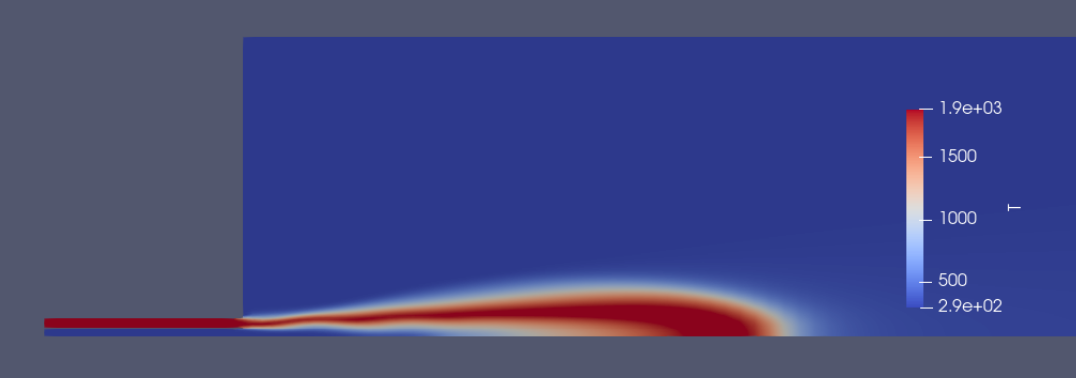
\includegraphics[width=0.95\linewidth]{figs/SandiaD/Screenshot from 2025-03-12 06-59-03.png}
    %\caption{The burner schematic in cross section view (a) and axis view (b) of the Sandia Flame D}
    \label{fig:domain}
\end{figure}

\begin{figure}[H]
    \centering
    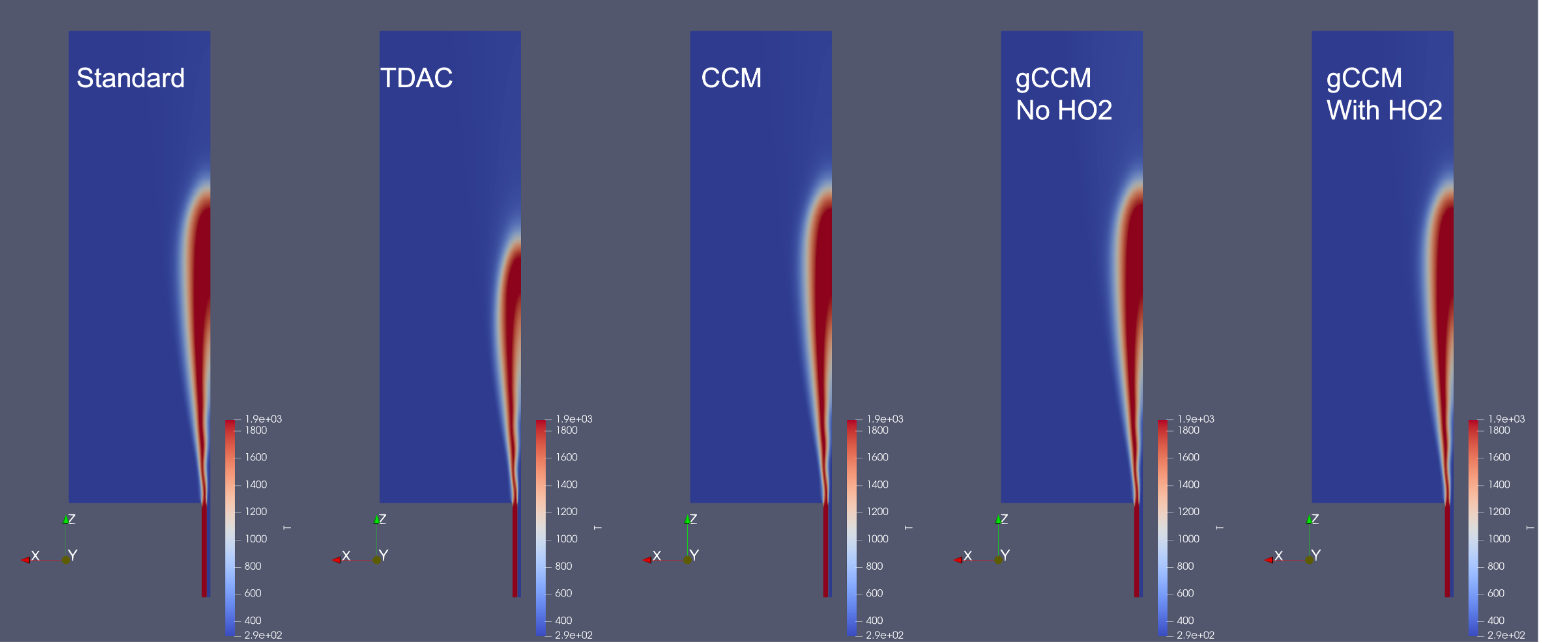
\includegraphics[width=0.95\linewidth]{figs/SandiaD/Screenshot from 2025-03-12 06-59-49.png}
    %\caption{The burner schematic in cross section view (a) and axis view (b) of the Sandia Flame D}
    \label{fig:domain}
\end{figure}

\begin{figure}[H]
    \centering
    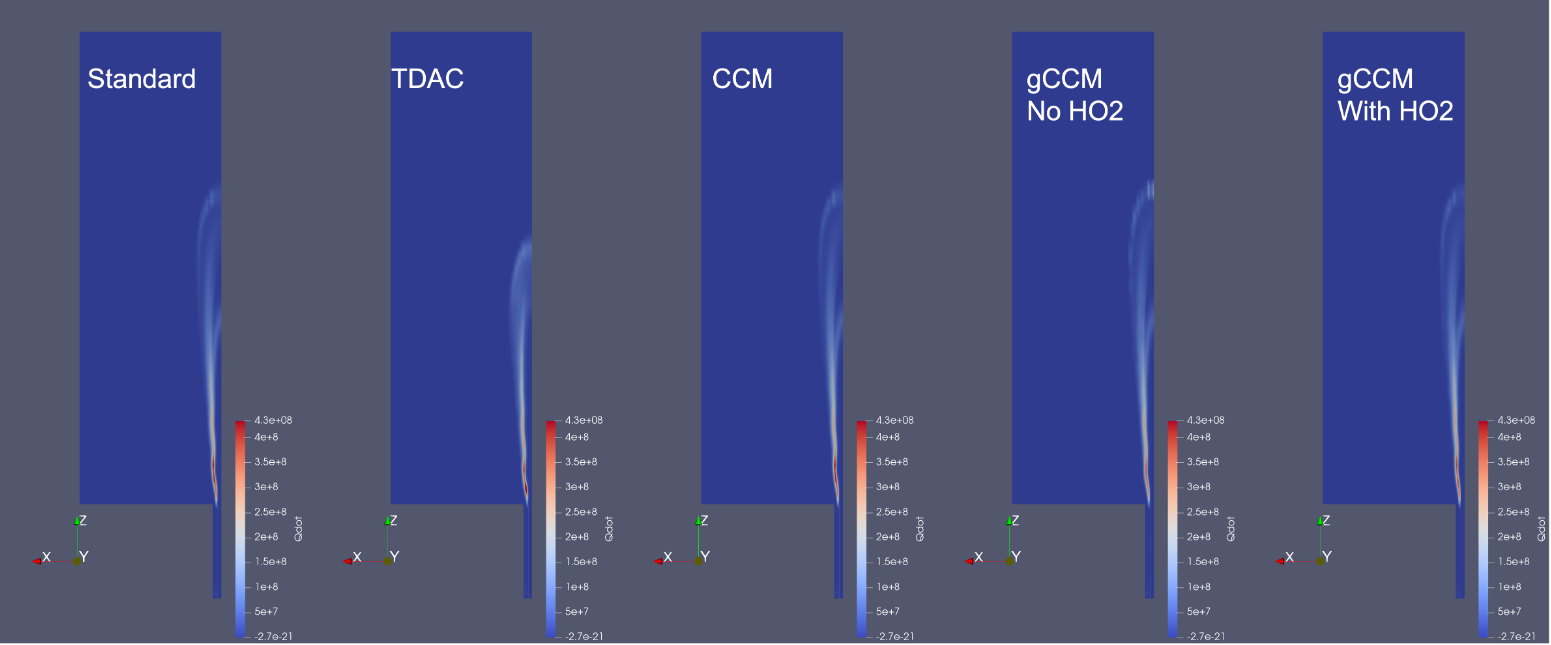
\includegraphics[width=0.95\linewidth]{figs/SandiaD/Screenshot from 2025-03-12 07-00-20.png}
    %\caption{The burner schematic in cross section view (a) and axis view (b) of the Sandia Flame D}
    \label{fig:domain}
\end{figure}

\begin{figure}[H]
    \centering
    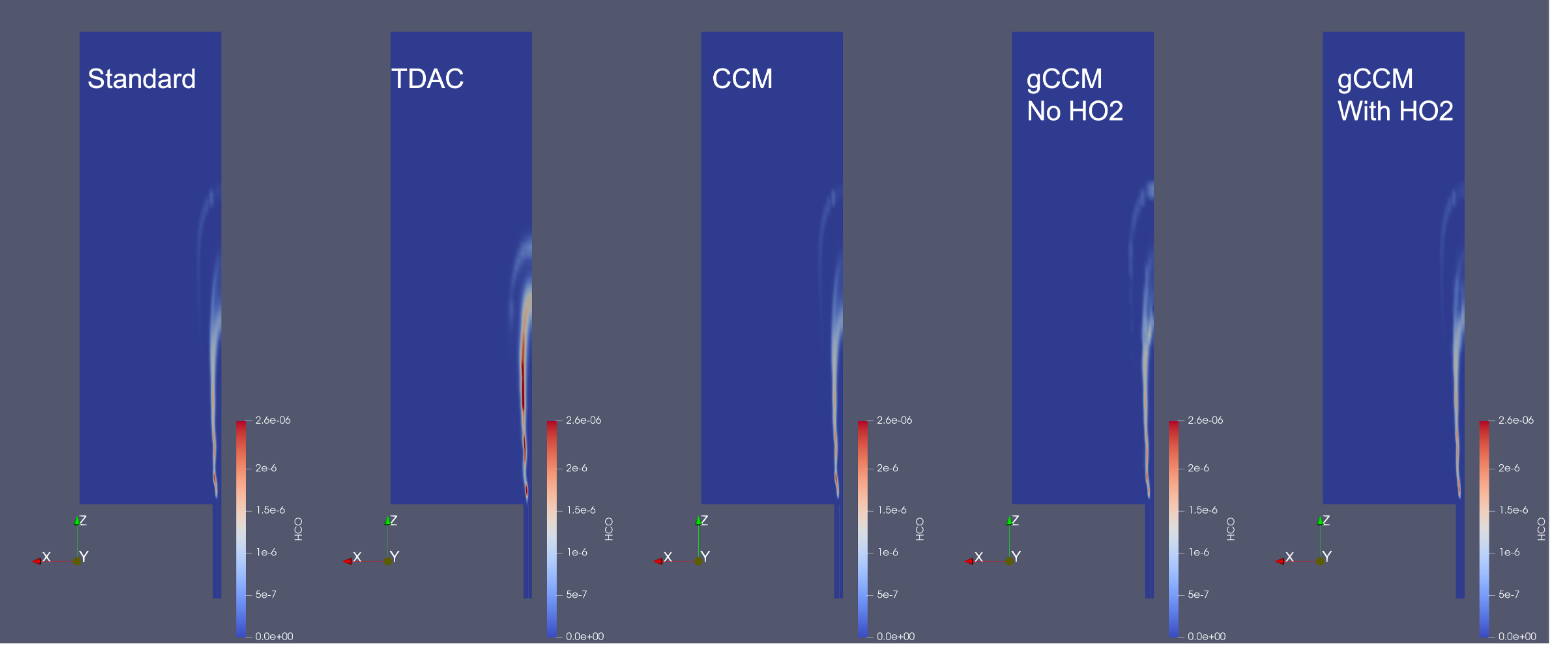
\includegraphics[width=0.95\linewidth]{figs/SandiaD/Screenshot from 2025-03-12 07-00-42.png}
    %\caption{The burner schematic in cross section view (a) and axis view (b) of the Sandia Flame D}
    \label{fig:domain}
\end{figure}

\begin{figure}[H]
    \centering
    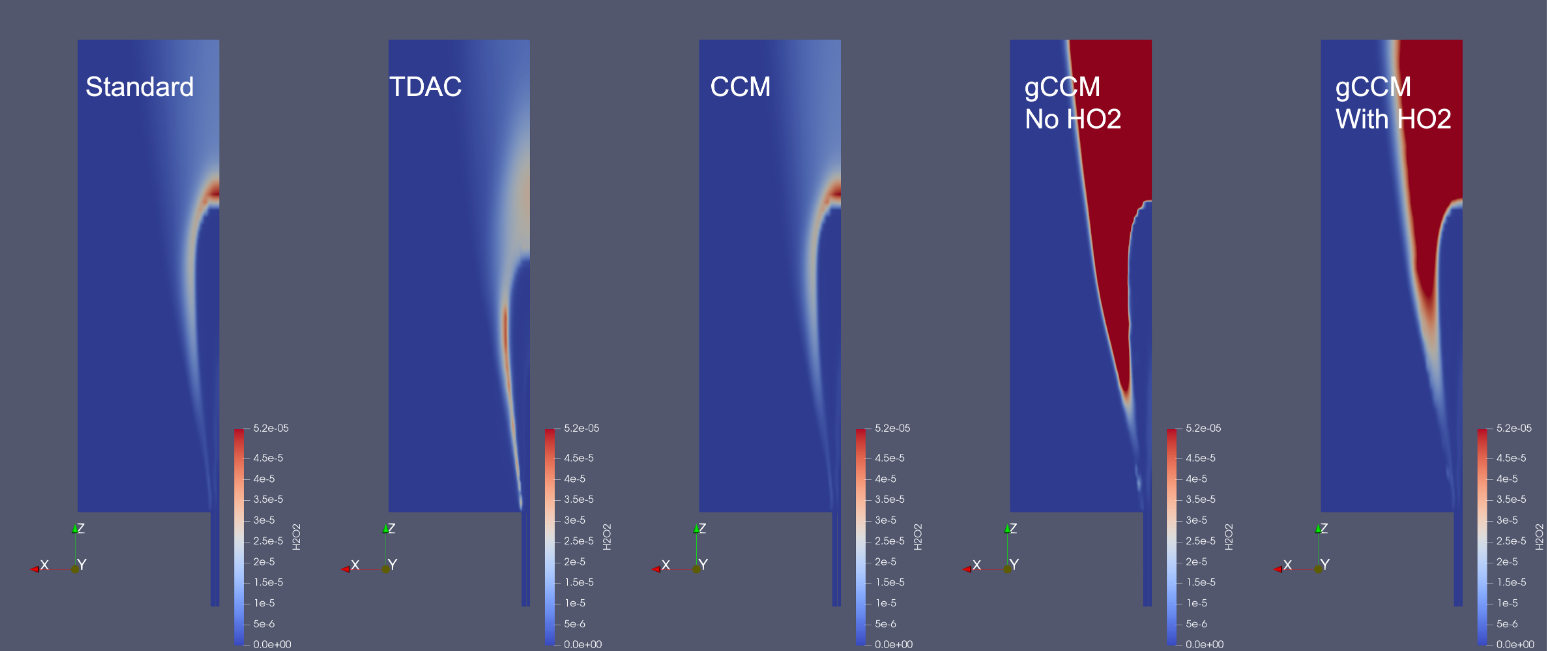
\includegraphics[width=0.95\linewidth]{figs/SandiaD/Screenshot from 2025-03-12 07-01-10.png}
    %\caption{The burner schematic in cross section view (a) and axis view (b) of the Sandia Flame D}
    \label{fig:domain}
\end{figure}

\begin{figure}[H]
    \centering
    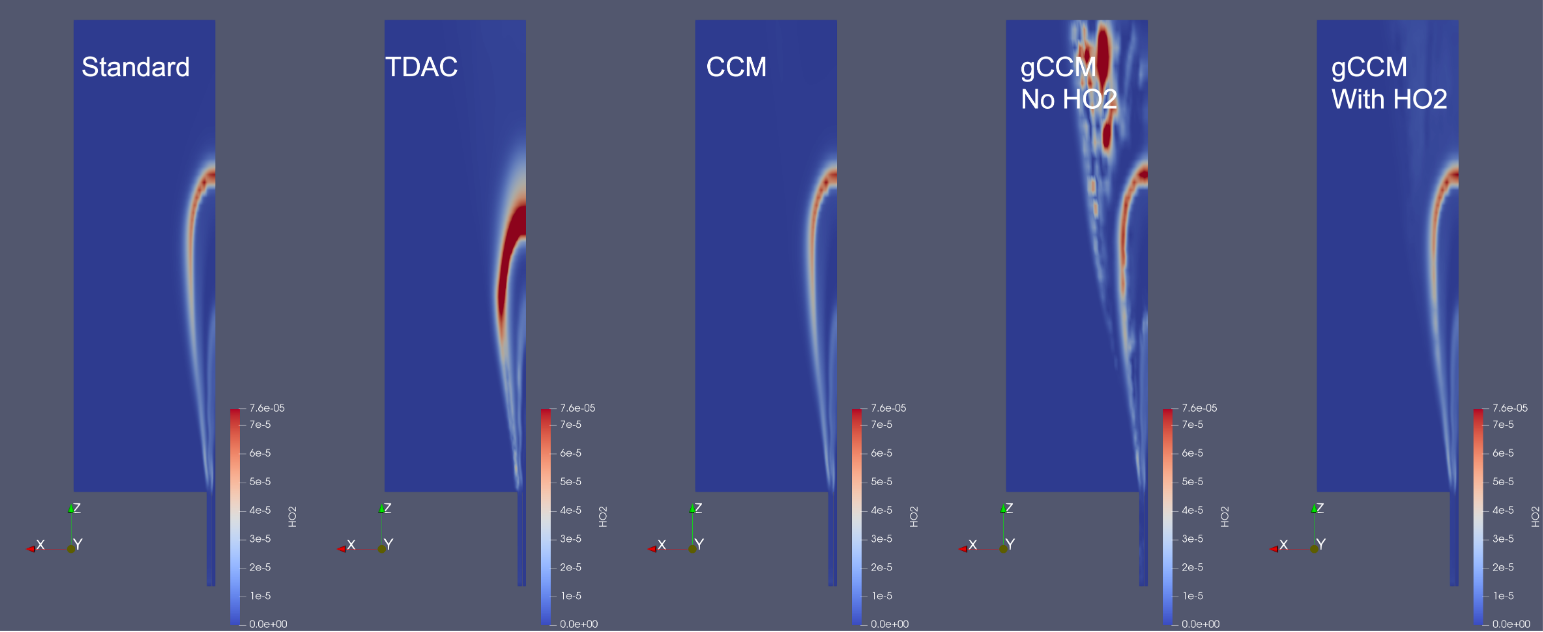
\includegraphics[width=0.95\linewidth]{figs/SandiaD/Screenshot from 2025-03-12 07-01-27.png}
    %\caption{The burner schematic in cross section view (a) and axis view (b) of the Sandia Flame D}
    \label{fig:domain}
\end{figure}

\begin{figure}[H]
    \centering
    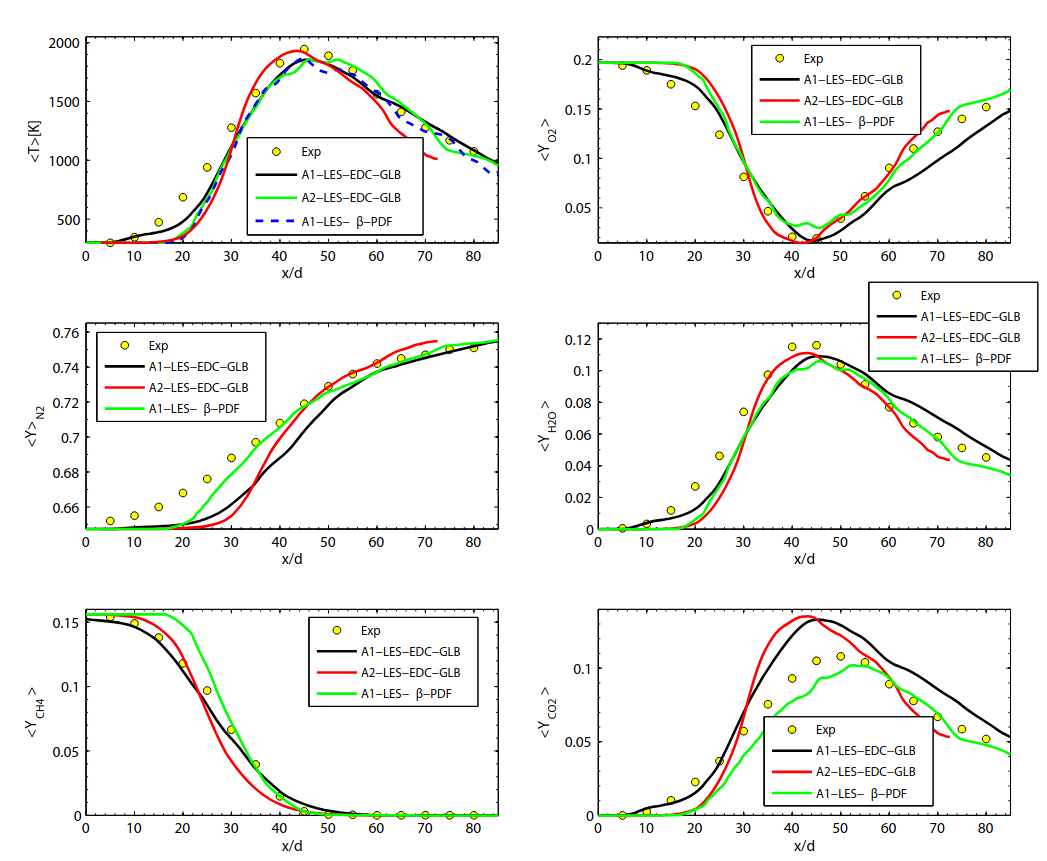
\includegraphics[width=0.95\linewidth]{figs/SandiaD/Screenshot from 2025-03-12 06-57-30.png}
    %\caption{The burner schematic in cross section view (a) and axis view (b) of the Sandia Flame D}
    \label{fig:domain}
\end{figure}

\begin{figure}[H]
    \centering
    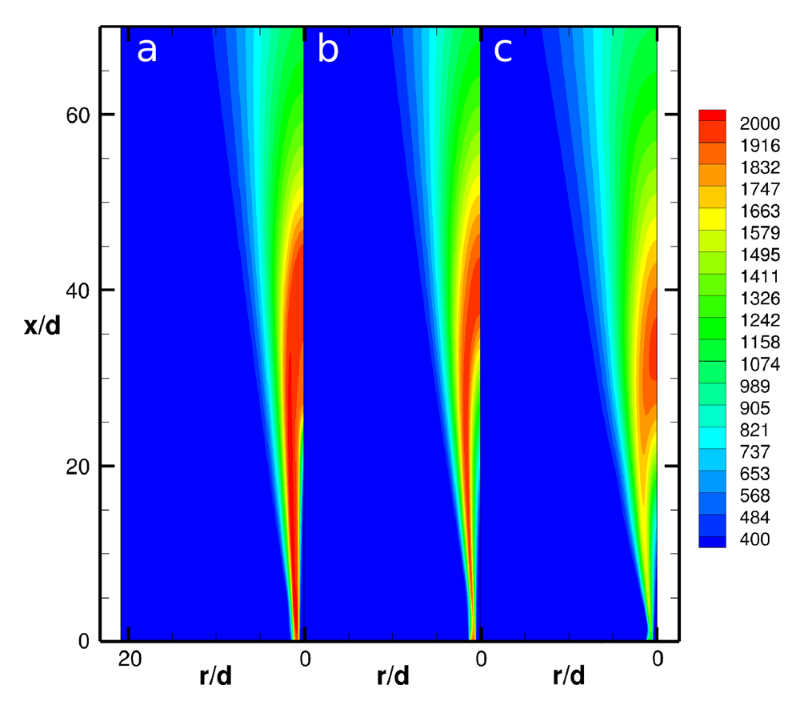
\includegraphics[width=0.95\linewidth]{figs/SandiaD/Screenshot from 2025-03-12 06-55-33.png}
    %\caption{The burner schematic in cross section view (a) and axis view (b) of the Sandia Flame D}
    \label{fig:domain}
\end{figure}

\begin{figure}[H]
    \centering
    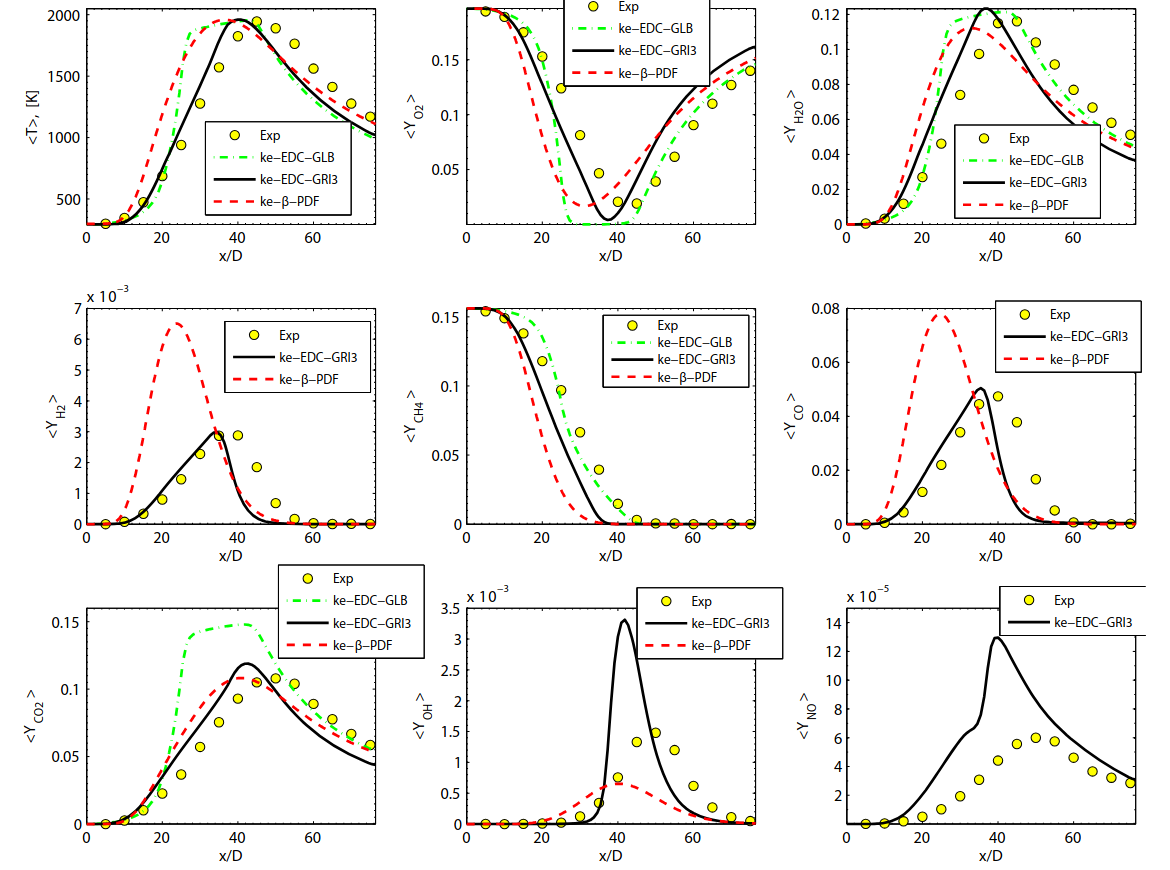
\includegraphics[width=0.95\linewidth]{figs/SandiaD/Screenshot from 2025-03-12 06-56-07.png}
    %\caption{The burner schematic in cross section view (a) and axis view (b) of the Sandia Flame D}
    \label{fig:domain}
\end{figure}

\begin{figure}[H]
    \centering
    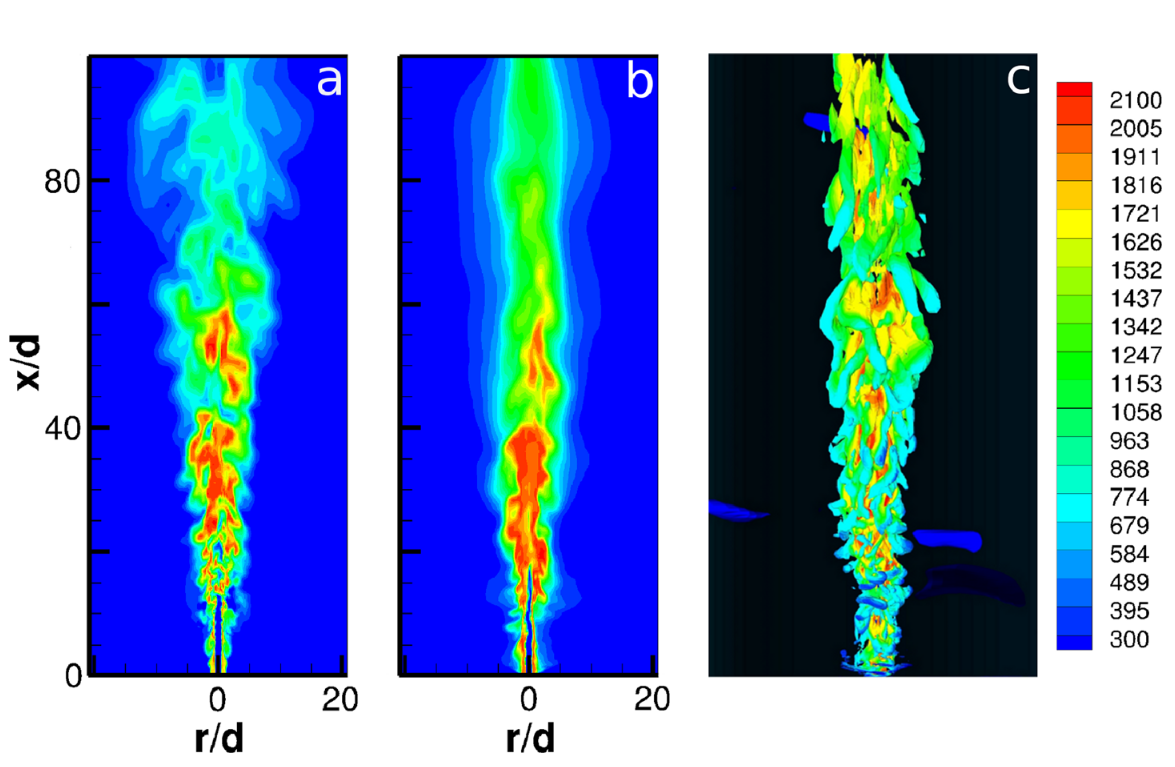
\includegraphics[width=0.95\linewidth]{figs/SandiaD/Screenshot from 2025-03-12 06-56-38.png}
    %\caption{The burner schematic in cross section view (a) and axis view (b) of the Sandia Flame D}
    \label{fig:domain}
\end{figure}

\begin{figure}[H]
    \centering
    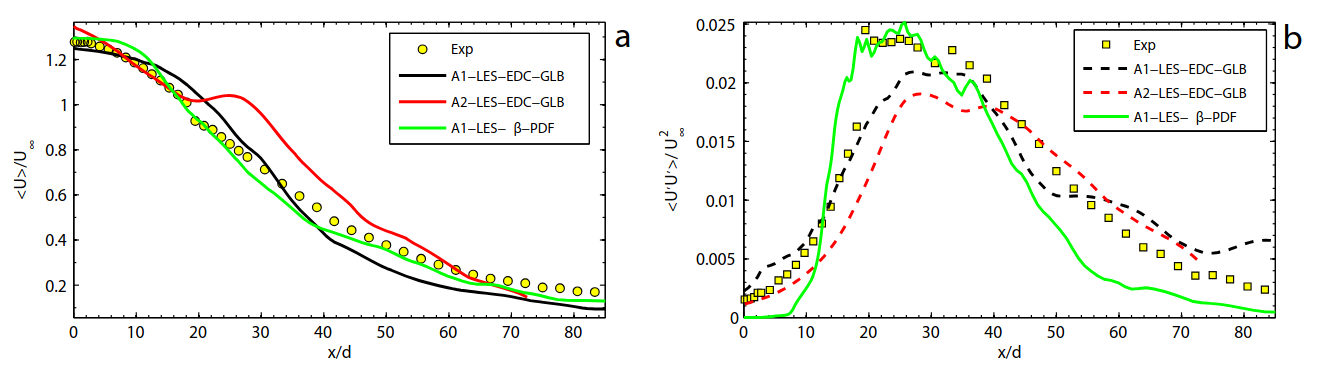
\includegraphics[width=0.95\linewidth]{figs/SandiaD/Screenshot from 2025-03-12 06-57-11.png}
    %\caption{The burner schematic in cross section view (a) and axis view (b) of the Sandia Flame D}
    \label{fig:domain}
\end{figure}

\begin{itemize}
    \item The test case models a turbulent premixed flame, which is a canonical problem in combustion research.
    \item It is derived from the Sandia Flame D experiments, involving methane-air combustion under well-defined conditions.
    \item The flame is stabilized by a bluff-body burner, creating a recirculation zone that stabilizes the flame.
\end{itemize}

%\subsection{Governing Equations}
\begin{itemize}
    \item The simulation solves the \textbf{Reynolds-Averaged Navier-Stokes (RANS)} equations coupled with a combustion model.
    \item A turbulence model, such as the \textbf{k-$\varepsilon$} or \textbf{k-$\omega$ SST} model, is typically used to account for turbulence effects.
    \item Combustion chemistry is modeled using simplified mechanisms, such as the \textbf{Eddy Dissipation Model (EDM)} or \textbf{Finite Rate Chemistry}.
\end{itemize}

\subsubsection*{OpenFOAM Chemistry Properties File}

Below is an example of an OpenFOAM \texttt{chemistryProperties} file:

\begin{lstlisting}[language=C++, caption={chemistryProperties}]
/*--------------------------------*- C++ -*----------------------------------*\
| =========                 |                                                 |
| \\      /  F ield         | OpenFOAM: The Open Source CFD Toolbox           |
|  \\    /   O peration     | Version:  2306                                  |
|   \\  /    A nd           | Website:  www.openfoam.com                      |
|    \\/     M anipulation  |                                                 |
\*---------------------------------------------------------------------------*/
// * * * * * * * * * * * * * * * * * * * * * * * * * * * * * * * * * * * * * //
FoamFile
{
    version         2;
    format          ascii;
    class           dictionary;
    object          chemistryProperties;
}

chemistryType
{
    solver          ode;
    method          TDAC;
}

chemistry       on;

importantSpecies
{
    CO2             ;
    H2O             ;
    CH4             ;
    O2              ;
}

initialChemicalTimeStep 1e-07;

odeCoeffs
{
    solver          seulex;
    absTol          1e-12;
    relTol          1e-07;
}

reduction
{
    active          on;
    log             on;
    tolerance       0.0001;
    method          DAC;
    initialSet
    {
        CO              ;
        CH4             ;
        HO2             ;
    }
    automaticSIS    off;
    fuelSpecies
    {
        CH4             1;
    }
}

tabulation
{
    active          on;
    log             on;
    printProportion off;
    printNumRetrieve off;
    tolerance       0.003;
    method          ISAT;
    scaleFactor
    {
        otherSpecies    1;
        Temperature     10000;
        Pressure        1e+15;
        deltaT          1;
    }
    maxNLeafs       5000;
    chPMaxLifeTime  1000;
    maxGrowth       100;
    checkEntireTreeInterval 500;
    maxDepthFactor  2;
    minBalanceThreshold 30;
    MRURetrieve     false;
    maxMRUSize      0;
    growPoints      true;
    maxNumNewDim    10;
}

// ************************************************************************* //
\end{lstlisting}

%\section*{OpenFOAM Combustion Properties File}

Below is an example of an OpenFOAM \texttt{combustionProperties} file:

\begin{lstlisting}[language=C++, caption={combustionProperties}]
/*--------------------------------*- C++ -*----------------------------------*\
| =========                 |                                                 |
| \\      /  F ield         | OpenFOAM: The Open Source CFD Toolbox           |
|  \\    /   O peration     | Version:  v2306                                 |
|   \\  /    A nd           | Website:  www.openfoam.com                      |
|    \\/     M anipulation  |                                                 |
\*---------------------------------------------------------------------------*/
FoamFile
{
    version     2.0;
    format      ascii;
    class       dictionary;
    object      combustionProperties;
}
// * * * * * * * * * * * * * * * * * * * * * * * * * * * * * * * * * * * * * //

combustionModel  EDC;

active  true;

EDCCoeffs
{
    version v2005;
}

// ************************************************************************* //
\end{lstlisting}

%\section*{OpenFOAM Radiation Properties File}

Below is an example of an OpenFOAM \texttt{radiationProperties} file:

\begin{lstlisting}[language=C++, caption={radiationProperties}]
/*--------------------------------*- C++ -*----------------------------------*\
| =========                 |                                                 |
| \\      /  F ield         | OpenFOAM: The Open Source CFD Toolbox           |
|  \\    /   O peration     | Version:  v2306                                 |
|   \\  /    A nd           | Website:  www.openfoam.com                      |
|    \\/     M anipulation  |                                                 |
\*---------------------------------------------------------------------------*/
FoamFile
{
    version     2.0;
    format      ascii;
    class       dictionary;
    object      radiationProperties;
}
// * * * * * * * * * * * * * * * * * * * * * * * * * * * * * * * * * * * * * //

radiation on;

radiationModel  P1;

P1Coeffs
{
    C               C [0 0 0 0 0 0 0] 0;
}

// Number of flow iterations per radiation iteration
solverFreq 1;

absorptionEmissionModel greyMeanAbsorptionEmission;

greyMeanAbsorptionEmissionCoeffs
{
    lookUpTableFileName      none;

    EhrrCoeff                0.0;

    CO2
    {
        Tcommon         200;   //Common Temp
        invTemp         true;   //Is the polynomio using inverse temperature.
        Tlow            200;   //Low Temp
        Thigh           2500;  //High Temp

        loTcoeffs       //coefss for T < Tcommon
        (
            0           //  a0            +
            0           //  a1*T          +
            0           //  a2*T^(+/-)2   +
            0           //  a3*T^(+/-)3   +
            0           //  a4*T^(+/-)4   +
            0           //  a5*T^(+/-)5   +
        );
        hiTcoeffs        //coefss for T > Tcommon
        (
            18.741
            -121.31e3
            273.5e6
            -194.05e9
            56.31e12
            -5.8169e15
        );

    }

    H2O
    {
        Tcommon         200;
        invTemp         true;
        Tlow            200;
        Thigh           2500;

        loTcoeffs
        (
            0
            0
            0
            0
            0
            0
        );
        hiTcoeffs
        (
            -0.23093
            -1.12390e3
             9.4153e6
            -2.99885e9
             0.51382e12
            -1.868e10
        );
    }

    CH4
    {
        Tcommon         200;
        Tlow            200;
        Thigh           2500;
        invTemp         false;

        loTcoeffs
        (
            0
            0
            0
            0
            0
            0
        );
        hiTcoeffs
        (
            6.6334
            -0.0035686
            1.6682e-8
            2.5611e-10
            -2.6558e-14
            0
        );
    }

    O2
    {
        Tcommon         200;
        invTemp         true;
        Tlow            200;
        Thigh           2500;

        loTcoeffs
        (
            0
            0
            0
            0
            0
            0
        );
        hiTcoeffs
        (
            0.1
            0
            0
            0
            0
            0
        );
    }


    N2
    {
        Tcommon         200;
        invTemp         true;
        Tlow            200;
        Thigh           2500;

        loTcoeffs
        (
            0
            0
            0
            0
            0
            0
        );
        hiTcoeffs
        (
            0.1
            0
            0
            0
            0
            0
        );
    }
}

scatterModel    none;

sootModel       none;

transmissivityModel none;

// ************************************************************************* //
\end{lstlisting}

\begin{lstlisting}[language=C++, caption={boundaryRadiationProperties}]
/*--------------------------------*- C++ -*----------------------------------*\
| =========                 |                                                 |
| \\      /  F ield         | OpenFOAM: The Open Source CFD Toolbox           |
|  \\    /   O peration     | Version:  v2306                                 |
|   \\  /    A nd           | Website:  www.openfoam.com                      |
|    \\/     M anipulation  |                                                 |
\*---------------------------------------------------------------------------*/
FoamFile
{
    version     2.0;
    format      ascii;
    class       dictionary;
    object      boundaryRadiationProperties;
}
// * * * * * * * * * * * * * * * * * * * * * * * * * * * * * * * * * * * * * //

".*"
{
    type            lookup;
    emissivity      1;
    absorptivity    0;
}

// ************************************************************************* //
\end{lstlisting}                                                                  

%\section*{OpenFOAM Thermophysical Properties File}

Below is the thermophysical properties configuration file used in OpenFOAM simulations:

\begin{lstlisting}[language=C++, caption={Thermophysical Properties File}]
/*--------------------------------*- C++ -*----------------------------------*\
| =========                 |                                                 |
| \\      /  F ield         | OpenFOAM: The Open Source CFD Toolbox           |
|  \\    /   O peration     | Version:  v2306                                 |
|   \\  /    A nd           | Website:  www.openfoam.com                      |
|    \\/     M anipulation  |                                                 |
\*---------------------------------------------------------------------------*/
FoamFile
{
    version     2.0;
    format      ascii;
    class       dictionary;
    object      thermophysicalProperties;
}
// * * * * * * * * * * * * * * * * * * * * * * * * * * * * * * * * * * * * * //

thermoType
{
    type            hePsiThermo;
    mixture         reactingMixture;
    transport       sutherland;
    thermo          janaf;
    energy          sensibleEnthalpy;
    equationOfState perfectGas;
    specie          specie;
}

inertSpecie N2;

chemistryReader foamChemistryReader;
foamChemistryFile "<constant>/reactionsGRI";
foamChemistryThermoFile "<constant>/thermo.compressibleGasGRI";

// ************************************************************************* //
\end{lstlisting}

\subsection*{OpenFOAM Radiation Properties File}
%%%%%%%%%%%%%%%%%%%%%%%%%%%%%%%%%%%%%%%%%%%%%
Then, radiationProperties and boundaryRadiationProperties are required to specify the radiation model’s properties. The radiationProperties is a dictionary that specifies the RTE solver and the spectral model under the constant folder, while the boundaryRadiationProperties is a dictionary that specifies the radiation model’s properties on the boundary. The radiationProperties is defined as below, which shows how to select P1 as the RTE solver and the grey mean absorption emission model as the spectral model. The absorption coefficient for each gas is the function of
temperature and is described as a polynomial. 

Below is an example of an OpenFOAM \texttt{radiationProperties} file:\\
\adjustbox{max width=\textwidth}{%
\begin{lstlisting}[language=C++, caption={radiationProperties}]
/*--------------------------------*- C++ -*----------------------------------*\
| =========                 |                                                 |
| \\      /  F ield         | OpenFOAM: The Open Source CFD Toolbox           |
|  \\    /   O peration     | Version:  v2306                                 |
|   \\  /    A nd           | Website:  www.openfoam.com                      |
|    \\/     M anipulation  |                                                 |
\*---------------------------------------------------------------------------*/
FoamFile
{
    version     2.0;
    format      ascii;
    class       dictionary;
    object      radiationProperties;
}
// * * * * * * * * * * * * * * * * * * * * * * * * * * * * * * * * * * * * * //

radiation on;

radiationModel  P1;

P1Coeffs
{
    C               C [0 0 0 0 0 0 0] 0;
}

// Number of flow iterations per radiation iteration
solverFreq 1;

absorptionEmissionModel greyMeanAbsorptionEmission;

greyMeanAbsorptionEmissionCoeffs
{
    lookUpTableFileName      none;

    EhrrCoeff                0.0;

    CO2
    {
        Tcommon         200;   //Common Temp
        invTemp         true;   //Is the polynomio using inverse temperature.
        Tlow            200;   //Low Temp
        Thigh           2500;  //High Temp

        loTcoeffs       //coefss for T < Tcommon
        (
            0           //  a0            +
            0           //  a1*T          +
            0           //  a2*T^(+/-)2   +
            0           //  a3*T^(+/-)3   +
            0           //  a4*T^(+/-)4   +
            0           //  a5*T^(+/-)5   +
        );
        hiTcoeffs        //coefss for T > Tcommon
        (
            18.741
            -121.31e3
            273.5e6
            -194.05e9
            56.31e12
            -5.8169e15
        );

    }

    H2O
    {
        Tcommon         200;
        invTemp         true;
        Tlow            200;
        Thigh           2500;

        loTcoeffs
        (
            0
            0
            0
            0
            0
            0
        );
        hiTcoeffs
        (
            -0.23093
            -1.12390e3
             9.4153e6
            -2.99885e9
             0.51382e12
            -1.868e10
        );
    }

    CH4
    {
        Tcommon         200;
        Tlow            200;
        Thigh           2500;
        invTemp         false;

        loTcoeffs
        (
            0
            0
            0
            0
            0
            0
        );
        hiTcoeffs
        (
            6.6334
            -0.0035686
            1.6682e-8
            2.5611e-10
            -2.6558e-14
            0
        );
    }

    O2
    {
        Tcommon         200;
        invTemp         true;
        Tlow            200;
        Thigh           2500;

        loTcoeffs
        (
            0
            0
            0
            0
            0
            0
        );
        hiTcoeffs
        (
            0.1
            0
            0
            0
            0
            0
        );
    }


    N2
    {
        Tcommon         200;
        invTemp         true;
        Tlow            200;
        Thigh           2500;

        loTcoeffs
        (
            0
            0
            0
            0
            0
            0
        );
        hiTcoeffs
        (
            0.1
            0
            0
            0
            0
            0
        );
    }
}

scatterModel    none;

sootModel       none;

transmissivityModel none;

// ************************************************************************* //
\end{lstlisting}}

For the boundaryRadiationProperties, a lookup model is selected, which assumes the boundary is grey. This assumption can be taken in most of the combustion cases.

\subsection*{OpenFOAM Simulation Script}
%%%%%%%%%%%%%%%%%%%%%%%%%%%%%%%%%%%%%
Below is the shell script used to set up and run an OpenFOAM simulation:

\adjustbox{max width=\textwidth}{%
\begin{lstlisting}[language=bash, caption={Simulation Script}]
#!/bin/sh
cd "${0%/*}" || exit                                # Run from this directory
. ${WM_PROJECT_DIR:?}/bin/tools/RunFunctions        # Tutorial run functions
#----------------------------------------------------------------------------

restore0Dir

runApplication chemkinToFoam \
    chemkin/grimech30.dat chemkin/thermo30.dat chemkin/transportProperties \
    constant/reactionsGRI constant/thermo.compressibleGasGRI

runApplication blockMesh

runApplication setFields

if isTest "$@"
then
    # Test without chemistry
    foamDictionary constant/chemistryProperties -entry chemistry -set off

    runApplication $(getApplication)

else
    # Run without chemistry until 1500 to let the flow field develop
    foamDictionary system/controlDict -entry writeInterval -set 1500

    foamDictionary system/controlDict -entry endTime -set 1500

    foamDictionary constant/chemistryProperties -entry chemistry -set off

    runApplication $(getApplication)

    # Run with chemistry until flame reaches its full size
    foamDictionary system/controlDict -entry writeInterval -set 100

    foamDictionary system/controlDict -entry endTime -set 5000

    foamDictionary constant/chemistryProperties -entry chemistry -set on

    runApplication -o $(getApplication)

fi
#------------------------------------------------------------------------------
\end{lstlisting}}

\subsubsection*{GRI-Mech 3.0: An Optimized Mechanism for Natural Gas Combustion}

\href{http://combustion.berkeley.edu/gri-mech/version30/text30.html}{GRI-Mech 3.0} is an optimized mechanism designed to model natural gas combustion, including NO formation and reburn chemistry. It is the successor to version 2.11 and represents another step in the continuing evolution of the mechanism. The optimization process aims to provide sound basic kinetics while furnishing the best combined modeling predictability of fundamental combustion properties.

\subsection*{Key Improvements in GRI-Mech 3.0}

Improvements were made in several categories:
\begin{itemize}
    \item Updating the kinetics with recent literature results.
    \item Including new and improved target experiments in the optimization process.
    \item Expanding the mechanism and target selection.
    \item Examining the sensitivity to thermodynamics.
\end{itemize}

Rate coefficient parameter changes are noted on the individual reaction web pages. Specific updates include:
\begin{itemize}
    \item Alterations to the CH kinetics important to prompt NO formation based on new measurements.
    \item New expressions for the H + O$_2$ reactions, CH$_3$ + O$_2$, CH$_2$O + H, and CH$_2$O decomposition.
    \item Recomputation of the methanol decomposition/chemical activation system.
    \item New branching paths for the oxidation steps CH$_3$ + O and CH$_2$ + O$_2$.
\end{itemize}

\subsection*{Additions to the Kinetics Mechanism}

Two main additions were made to the kinetics mechanism, involving the inclusion of four new species:
\begin{itemize}
    \item \textbf{Acetaldehyde and vinoxy chemistry}: These were added to better describe ethylene oxidation and are now included among the Ox + C$_2$H$_y$ reaction products.
    \item \textbf{Propane kinetics}: A minimal set of propane kinetics was included to model this species as a minor constituent, reflecting the presence of propane (and some higher hydrocarbons) in natural gas.
\end{itemize}

\subsection*{New Target Additions}
%%%%%%%%%%%%%%%%%%%%%%%%%%%%%%%%%%
Other new target additions include:
\begin{itemize}
    \item A series of shock tube observations sensitive to the oxidation of the formaldehyde intermediate.
    \item Shock tube, low-pressure flame, and flow reactor experiments concerning prompt NO formation and reburn.
    \item Targets related to the shortening of methane shock tube ignition delays by small amounts of propane or ethane.
    \item Revised and expanded sets of shock tube ignition delays and laminar flame speeds.
\end{itemize}

Many of these changes reflect the acquisition of improved data.

\subsection*{Mechanism Details}
%%%%%%%%%%%%%%%%%%%%%%%%%%%%%%%
The new mechanism contains:
\begin{itemize}
    \item 325 reactions (3 are duplicates because the sum of two rate parameter expressions is required).
    \item 53 species (including argon).
\end{itemize}

The final optimization to 77 targets altered 31 rate parameters.

\subsection*{Major Results of the Optimization}
%%%%%%%%%%%%%%%%%%%%%%%%%%%%%%%%%%%%%%%%%%%%%%%
The major results of the new mechanism optimization are summarized below:

\begin{enumerate}
    \item Deviations from the target values are generally less than previously. (The chi-square for the sum of common retained targets dropped from 0.96 to 0.81.)
    \item Similar final values for the key rates CH$_3$ + H, CH$_3$ + OH, and CH$_3$ + O$_2$ were found.
    \item Including formaldehyde target optimization did not require changes to the new expressions for the sensitive CH$_2$O + M and CH$_2$O + H rate constants. Other changes consistent with the rest of the targets sufficed.
    \item Significant thermodynamics sensitivity was found only for HCN in some targets, leading to an alteration of the JANAF value.
    \item A new, improved low-pressure flame prompt NO target results in higher values for CH + N$_2$, and predictions of increased prompt NO.
    \item New lower experimental flame speed values remain overpredicted by the optimized mechanism. Transport uncertainties have not yet been examined in this regard. Note also that some computational inaccuracies exist in the flame speed computations used for the GRI-Mech 1.2 target optimization.
\end{enumerate}

\section*{GRI-Mech 3.0 Optimization Details}
%%%%%%%%%%%%%%%%%%%%%%%%%%%%%%%%%%%%%%%%%%%%
GRI-Mech 3.0 began with 81 targets and 103 variables. The final optimization considered 77 targets and varied 32 parameters. Four targets were omitted when found inconsistent with other optimization targets, and 71 variables were frozen at starting values when judged to provide only insignificant improvements to overall target fits if varied.

\subsection*{Key Observations in the Optimization Process}
%%%%%%%%%%%%%%%%%%%%%%%%%%%%%%%%%%%%%%%%%%%%%%%%%%%%%%%%%%
The majority of high-temperature methane shock tube and flame speed targets drive an increase in only three rate constants:
\begin{itemize}
    \item Methane recombination.
    \item Two CH$_3$ + O$_2$ rate parameters.
\end{itemize}
These assume optimized values close to those in mechanism 1.2. In the final optimization run, we decided to limit the multiplier for CH$_3$ + O$_2$ = OH + CH$_2$O to that for the O + CH$_3$O channel. It was not necessary or particularly advantageous to allow the optimization to adjust other key sensitive rate constants:
\begin{itemize}
    \item H + O$_2$,
    \item OH + CO,
    \item O + CH$_3$,
    \item HCO decomposition,
    \item CH$_2$ + O$_2$,
    \item OH + CH$_3$.
\end{itemize}
These remain at their initial values. Including the H + O$_2$ chain branching step and OH + CO in the optimization would decrease these rate constants, improving flame speed predictions at 1 atm but at the expense of greater disagreement at high pressure and for shock tube species profiles. Thus, we decided not to alter these rate constants.

For OH + CH$_3$ and HCO + M reactions, the optimization suggested multipliers of 1.0 (no change). For O + CH$_3$ and CH$_2$ + O$_2$, the optimization is more inclined to alter the product branching ratios than overall rates, but still gives negligible improvement.

\subsection*{Target-Specific Improvements}
%%%%%%%%%%%%%%%%%%%%%%%%%%%%%%%%%%%%%%%%%%
Many of the other reaction rate constant changes in the optimization are driven by major improvements in matching smaller subsets of targets:
\begin{itemize}
    \item Propane results are improved by decreasing $k(312)$.
    \item Ethane targets influence $k(74)$, $k(158)$, and $k(159)$. However, the ethane kinetics also affect the methane (especially CH$_3$) targets.
\end{itemize}
This isolation of select target-reaction subsets is still apparent in the limited list of nitrogen targets, as it was for version 2.11, although several new results have been added. Compare the individual target page sensitivities for details.

\subsection*{CH$_2$O Targets}
%%%%%%%%%%%%%%%%%%%%%%%%%%%%%
To accommodate the new CH$_2$O targets in the 3.0 optimization, it was only necessary to optimize the HO$_2$ + CH$_2$O and HCO + O$_2$ rate constants. Adjustments to the key H + CH$_2$O and decomposition reactions (reparameterized for the 3.0 round starting mechanism) were not needed. Eiteneer et al. (1998) needed to suggest some modifications to these rate constants when they first considered their data as an addendum to version 1.2 optimization results.

\subsection*{Prompt NO Targets}
%%%%%%%%%%%%%%%%%%%%%%%%%%%%%%%%%
Another cluster of rate parameters ($k(49)$, $k(125)$, $k(126)$, $k(289)$, $k(240)$, $k(246-248)$) influences the optimized results for new CH measurements and prompt NO targets. The starting kinetics were also revised based on new data, especially regarding the CH + O$_2$ and H$_2$ reaction systems.

\subsection*{Limited Target-Specific Optimizations}
%%%%%%%%%%%%%%%%%%%%%%%%%%%%%%%%%%%%%%%%%%%%%%%%%%%
We permitted some rather target-specific optimizations in limited cases where considerable improvement could be made:
\begin{itemize}
    \item Increasing $k(119)$ improves the prediction of the IG.St1a ignition delay and the high-pressure flame speeds, as does lowering OH + HO$_2$. This speeds up high-pressure, low-temperature chain branching.
    \item Flame speed improvements also largely dictate the modifications to the HCO + O$_2$ and H$_2$O rate constants.
    \item Changing H + O$_2$ + H$_2$O and the H + HO$_2$ branching ratio improves methane and hydrogen flame speed predictions.
\end{itemize}
These four alterations all serve to reduce chain branching and lower the atmospheric pressure flame speed overpredictions.

\subsection*{Rate Constant Limits}
%%%%%%%%%%%%%%%%%%%%%%%%%%%%%%%%%%
In some cases, usually involving these target-specific rates or some nitrogen targets, rate constants were adjusted to the full limits we judged prudent, although larger changes would improve agreement more. However, changes to the allowed limits did not occur in the optimization for the key core hydrocarbon kinetics ($k(52)$, $k(119)$, $k(155)$, $k(156)$, $k(158)$, $k(159)$, and $k(168)$). In fact, including the CH$_3$ + CH$_3$ steps in the optimization resulted in smaller changes to the other important rate parameters.

\subsection*{Propane Ignition Delays}
%%%%%%%%%%%%%%%%%%%%%%%%%%%%%%%%%%%%%
We originally included some additional targets involving ignition delays in propane fuel mixtures from Borisov et al., but large deviations were observed for all optimization runs for two of the four targets. Within the context of our very limited C-3 kinetics, these results are inconsistent with the other targets and hence were omitted.

\subsection*{Comparison of Rate Constants}
%%%%%%%%%%%%%%%%%%%%%%%%%%%%%%%%%%%%%%%%%%
The table below compares rate constant values at 1 atm, 1500 K for many of the key reactions, giving a ratio for GRI-Mech 3.0 vs. 2.11. Significant changes are highlighted and may be due to new kinetic results, the new optimization, or a combination.

%\begin{table}[H]
%\centering
%\begin{tabular}{ccc}
%\toprule
%Reaction \# & $k(3.0)/k(2.11)$ & Reaction \# & $k(3.0)/k(2.11)$ & Reaction \# & $k(3.0)/k(2.11)$ \\
%\midrule
%36 & 2.32 & 99 & 1.00 & 159 & 0.50 \\
%38 & 0.98 & 119 & 1.89 & 166 & 0.84 \\
%52 & 1.16 & 125 & 2.03 & 168 & 1.76 \\
%54 & 2.49 & 155 & 0.76 & 178 & 0.77 \\
%58 & 1.49 & 156 & 1.41 & 180 & 0.59 \\
%74 & 0.50 & 155-6 & 1.09 & 240 & 1.98 \\
%97 & 0.89 & 158 & 1.09 & 246-8 & 0.82 \\
%\bottomrule
%\end{tabular}
%\caption{Comparison of rate constants at 1 atm, 1500 K for GRI-Mech 3.0 vs. 2.11.}
%\end{table}

%
\subsection{The Aachen Bomb}
%%%%%%%%%%%%%%%%%%%%%%%%%%%%

The \href{https://develop.openfoam.com/Development/openfoam/-/tree/OpenFOAM-v2106/tutorials/lagrangian/sprayFoam/aachenBomb}{AachenBomb} testcase is the simulation of combustion inside a constant volume chamber that mimics the begining of power stroke in a 4 stroke engine. The experimental setup of the combustion chamber is in RWTH Aachen university, and the operating conditions are in accordance with the Engine Combustion Network\footnote{https://crf.sandia.gov/research/engine-combustion.}

As mentioned before the geometry of AachenBomb case is similar to the constant volume combustion chamber in RWTH Aachen. The geometry is a cuboid with height(+ve y-axis) 0.1 m and base 0.02x0.02 m (figure 2.1). The injector is placed 5 mm below the top of the chamber (at a height 0.995 m from the bottom plane) in order to avoid boundary effects on the injected fluid. The fluid
that is injected is n-Heptane (C7H16).

% Table 2.3: Input files for the aachenBomb case
\begin{table}[H]
    \centering
    \caption{Input files for the aachenBomb case}
    \label{tab:aachenbomb-input-files}
    \begin{tabular}{lp{10cm}}
        \toprule
        \textbf{Input file} & \textbf{Functionality} \\
        \midrule
        sprayCloudProperties & Contains inputs for the Lagrangian spray model. \\
        thermophysicalProperties & Contains inputs for the thermophysical models. \\
        radiationProperties & Contains inputs for radiation, absorption-emission, and soot models. \\
        ChemistryProperties & Specifies the chemistry solver and option to switch on/off the chemical reactions. \\
        combustionProperties & Contains inputs for the combustion model and option to switch on/off combustion. \\
        turbulenceProperties & Contains inputs for the turbulence model and option to switch on/off turbulence. \\
        \bottomrule
    \end{tabular}
\end{table}

\begin{enumerate}
    \item Prepare the case directory by copying a tutorial \\ (e.g., \texttt{tutorials/combustion/reactingFoam/ras/counterFlowFlame2D}).
    \item Modify configuration files (\texttt{controlDict}, \texttt{fvSchemes}, \texttt{fvSolution}).
    \item Run the simulation:
\begin{lstlisting}[language=bash, caption={Running the Simulation.}]
blockMesh
reactingFoam
\end{lstlisting}
    \item Post-process results using ParaView.
\end{enumerate}

%\subsection{MB18 gas/spray penetration}
%%%%%%%%%%%%%%%%%%%%%%%%%%%%%%%%%%%%%%%
The primary concern of this project is fire modelling and suppression. In this \href{https://develop.openfoam.com/exafoam/wp2-validation/-/tree/master/lagrangian/sprayFoam/gasSprayPenetration?ref_type=heads}{MB18 gas/spray penetration testcase}, we deal with the main mechanism for fire suppression, namely via water spray, by which the liquid and evaporated species are mechanisms to reduce the enclosure temperature and/or directly to suppress the fire and source. This case uses the OpenFOAM Lagrangian solver to track the spray droplets trajectory through the mesh, coupled with the flow solver in exchange of mass (phase change), momentum (droplet and continuum fluid drag forces) and energy (needed to evaporate the liquid phase)

Validation of the following solvers within the Eulerian-Lagrangian framework
in terms of macroscopic and microscopic spray development and vaporisation:
\href{https://develop.openfoam.com/Development/openfoam/-/tree/master/applications/solvers/lagrangian/sprayFoam/sprayFoam.C}{sprayFoam}.

\subsubsection*{Methodology}
The test case is based on the Engine Combustion Network (ECN) workshop's \textit{Spray-A} experimental configuration \cite{ref1}. The \textit{Spray-A} case is a basic single-hole non-reacting spraying-into-a-closed-volume configuration; "well-characterized, but is likely non-cavitating (and thus, unrealistic)" \cite{ref2}.

\subsubsection*{Metrics}
The metrics to quantify the validations are \cite{ref3}:
\begin{itemize}
    \item Macroscopic spray development:
    \begin{itemize}
        \item Liquid penetration vs time (liquid-length)
        \item Vapor-phase penetration vs time
        \item Mixture fraction profiles (both axial and radial)
        \item Extinction profiles (both axial and radial)
    \end{itemize}
    \item Microscopic spray development:
    \begin{itemize}
        \item Spray penetration and velocity in the near-field
        \item Spreading angle
        \item Microscopic features (fuel ligaments, droplet formation etc.)
    \end{itemize}
\end{itemize}

\subsubsection*{Benchmarks}
The database of the experiments can be accessed through the \href{https://ecn.sandia.gov/ecn-data-search/}{ECN search engine}.

%The experimental configurations that were used in this study:
\begin{figure}[H]
    \centering
    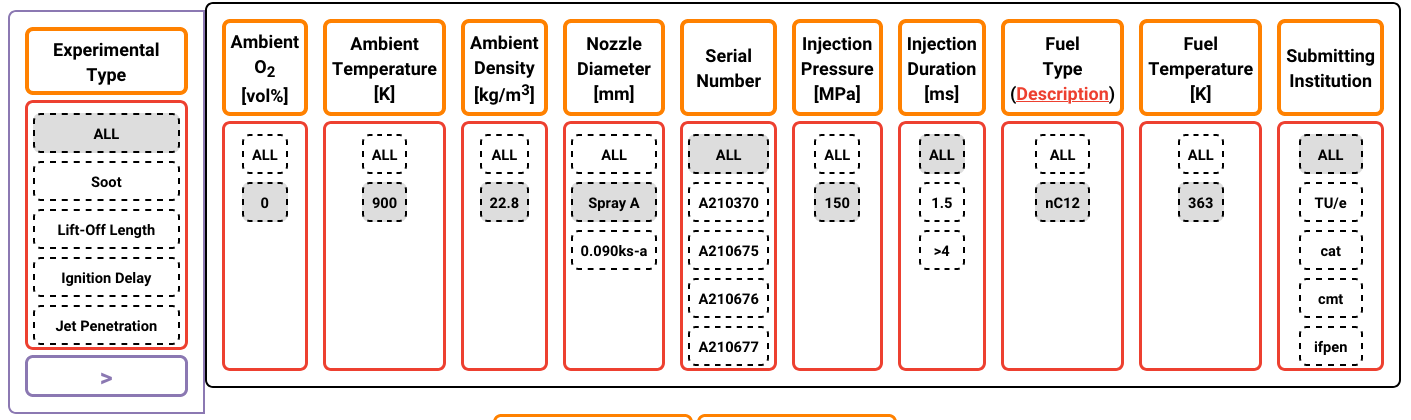
\includegraphics[width=0.9\linewidth]{figs/MB18/experiment-search-criteria.png}
    \caption{Experimental datasets used in this study.}
    \label{fig:enter-label}
\end{figure}

%The experimental datasets that were used in this study:
\begin{figure}[H]
    \centering
    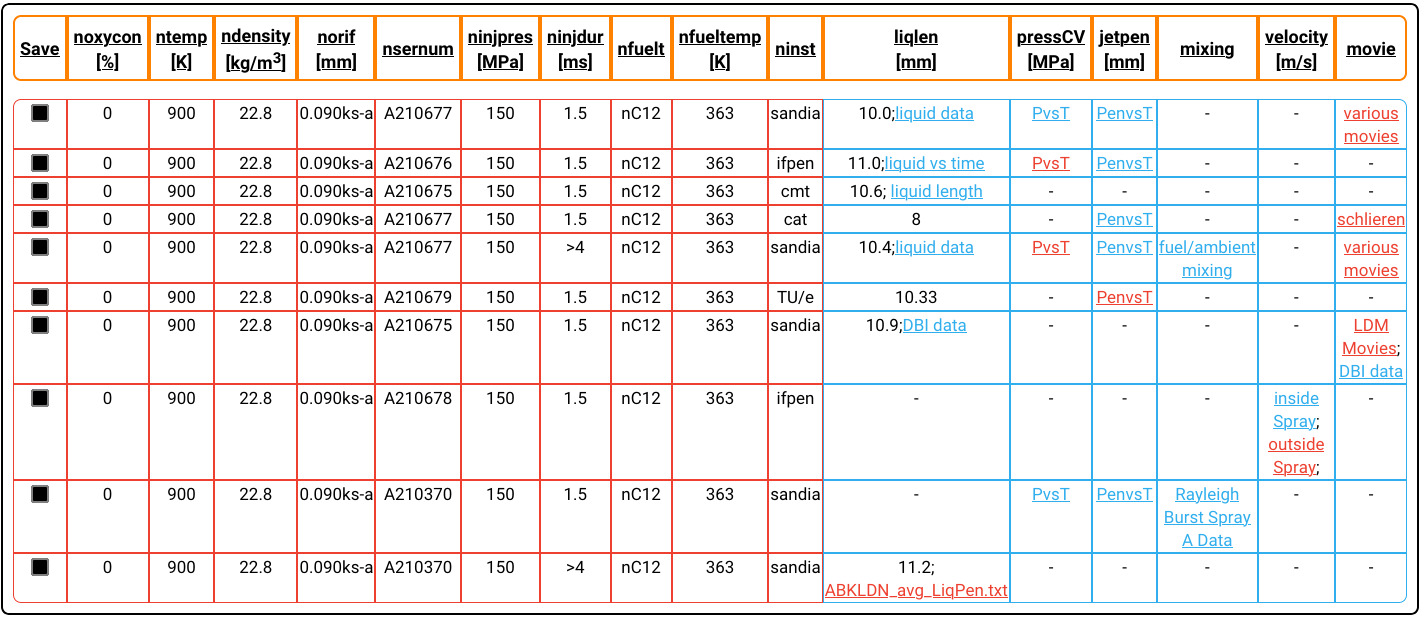
\includegraphics[width=0.9\linewidth]{figs/MB18/experiment-search-output.png}
    \caption{Experimental configurations used in this study.}
    \label{fig:enter-label}
\end{figure}

\subsubsection*{Definitions}
\paragraph{Liquid Penetration:} 
"Maximum distance from the nozzle outlet to the farthest axial position where projected liquid volume in the cross-stream direction decreases to a specific value. The projected liquid volume is defined as $\mathrm{PLV} = \int \mathrm{LVF} dy$, where $\mathrm{LVF}$ is liquid volume fraction and $\mathrm{PLV}$ is projected liquid volume. Two values for $\mathrm{PLV}$ are considered:" \cite{ref6}

\begin{equation}
    \int \mathrm{LVF} \, dy = 0.2\text{e-}3 \, [\mathrm{mm}^3 \, \text{liquid} / \mathrm{mm}^2]
\end{equation}

\begin{equation}
    \int \mathrm{LVF} \, dy = 2.0\text{e-}3 \, [\mathrm{mm}^3 \, \text{liquid} / \mathrm{mm}^2]
\end{equation}

In some studies, such as in \cite{ref7}, the liquid spray penetration "is defined as the maximum distance from the injector nozzle to the farthest axial position where 95\% of the liquid mass is found."

\paragraph{Vapor Penetration:} 
"Maximum distance from the nozzle outlet to where the fuel mass fraction (or mixture fraction (author's note: if the system is reacting)) is 0.1\%." \cite{ref6}

\subsubsection*{Physical Domain}
A constant volume vessel of cubic shape.

\subsubsection*{Physical Modelling}
Reference quantities \cite{ref1, ref7}:

\subsubsection*{Ambient Conditions (Gas)}
\begin{center}
\begin{tabular}{ll}
\hline
Metric & Value \\
\hline
Composition (by volume) & $0.00\%\,\mathrm{O}_2$, $6.52\%\,\mathrm{CO}_2$, $3.77\%\,\mathrm{H}_2\mathrm{O}$, $89.71\%\,\mathrm{N}_2$ \\
Temperature & $\mathrm{T}_{amb} = 900 \, [\mathrm{K}]$ \\
Pressure & $p_{amb} \approx 6.0 \, [\mathrm{MPa}]$ \\
Density & $\rho_{amb} = 22.8 \, [\mathrm{kg}/\mathrm{m}^3]$ \\
Velocity & Near-quiescent, less than $1 \, [\mathrm{m}/\mathrm{s}]$ \\
\hline
\end{tabular}
\end{center}

\subsubsection*{Injection Conditions (Liquid)}
\begin{center}
\begin{tabular}{ll}
\hline
Metric & Value \\
\hline
Fuel type & n-dodecane ($n\text{-}\mathrm{C}_{12}\mathrm{H}_{26}$) \\
Fuel temperature & $\mathrm{T}_{inj} = 363 \, [\mathrm{K}]$ \\
Density & $\rho = 713.13 \, [\mathrm{kg}/\mathrm{m}^3]$ \\
Injection duration(s) & $t_{inj} = 1.5 \, [\mathrm{ms}]$ and $t_{inj} = 6 \, [\mathrm{ms}]$ \\
Injection mass & $m_{inj} = 3.56 \, [\mathrm{mg}]$ \\
Injection pressure & $m_{inj} = 150 \, [\mathrm{MPa}]$ \\
Injection direction & Axial \\
Discharge coefficient & $c_{discharge} = 0.89 \, [-]$ \\
Mass flow rate of injection vs time & \href{resources/massFlowRateOfInjection_1.5}{1.5 ms} \\
\hline
\end{tabular}
\end{center}

Derived quantities \cite{ref7}:\\
\begin{center}
\begin{tabular}{ll}
\hline
Metric & Value \\
\hline
Turbulent kinetic energy & $k = 0.735 \, [\mathrm{m}^2/\mathrm{s}^2]$ \\
Turbulent kinetic energy dissipation rate & $\epsilon = 5.67 \, [\mathrm{m}^2/\mathrm{s}^3]$ \\
\hline
\end{tabular}
\end{center}

\subsubsection*{Spray Models}
The officially-recommended baseline spray models were reported in \cite{ref3, ref5}:

\begin{center}
\adjustbox{max width=\textwidth}{%
\begin{tabular}{ll}
\hline
Topic & Model \\
\hline
RANS closure model & RNG k-epsilon model \\
Injection & Blob injection \\
Atomisation and primary/secondary breakups & Kelvin-Helmholtz instability model and Rayleigh-Taylor accelerative instability mode (i.e., KHRT) \\
Collision & O'Rourke model \\
Drag & Dynamic model \\
Evaporation & Frossling model \\
Heat transfer & Ranz-Marshall model \\
Dispersion & Stochastic model \\
\hline
\end{tabular}}
\end{center}

The spray models being used in this study were listed as follows:

\begin{center}
\adjustbox{max width=\textwidth}{%
\begin{tabular}{ll}
\hline
Topic & Model \\
\hline
RANS closure model & RNG k-epsilon model \\
Injection & Injection: coneNozzleInjection Cone angle: $22^\circ$ \\
Atomisation and primary/secondary breakups & ReitzKHRT \\
Collision & None \\
Drag & sphereDrag \\
Evaporation & liquidEvaporationBoil \\
Heat transfer & RanzMarshall \\
Dispersion & stochasticDispersionRAS \\
Size distribution & Rosin Rammler \\
\hline
\end{tabular}}
\end{center}

\subsubsection*{Numerical Domain Modelling}
Dimensions: $(\mathrm{x}, \mathrm{y}, \mathrm{z}) = (180, 180, 180) \, [\mathrm{mm}]$

\begin{itemize}
    \item x: Longitudinal direction (mean spray direction)
    \item y: Spanwise direction
    \item z: Vertical direction
\end{itemize}

Injector characteristics:
\begin{itemize}
    \item Number of injector holes: 1 (axial)
    \item Nominal injector nozzle diameter: $D = 0.09 \, [\mathrm{mm}]$
\end{itemize}

\subsubsection*{Numerical Domain Discretisation}
Spatial domain discretisation: See \texttt{system/blockMeshDict}. (nref=1)

\begin{itemize}
    \item $\Delta x_{min} = 0.25 \, [\mathrm{mm}]$ (in spray liquid core region)
    \item $\Delta x_{max} = 4.0 \, [\mathrm{mm}]$
\end{itemize}

\begin{figure}[H]
    \centering
    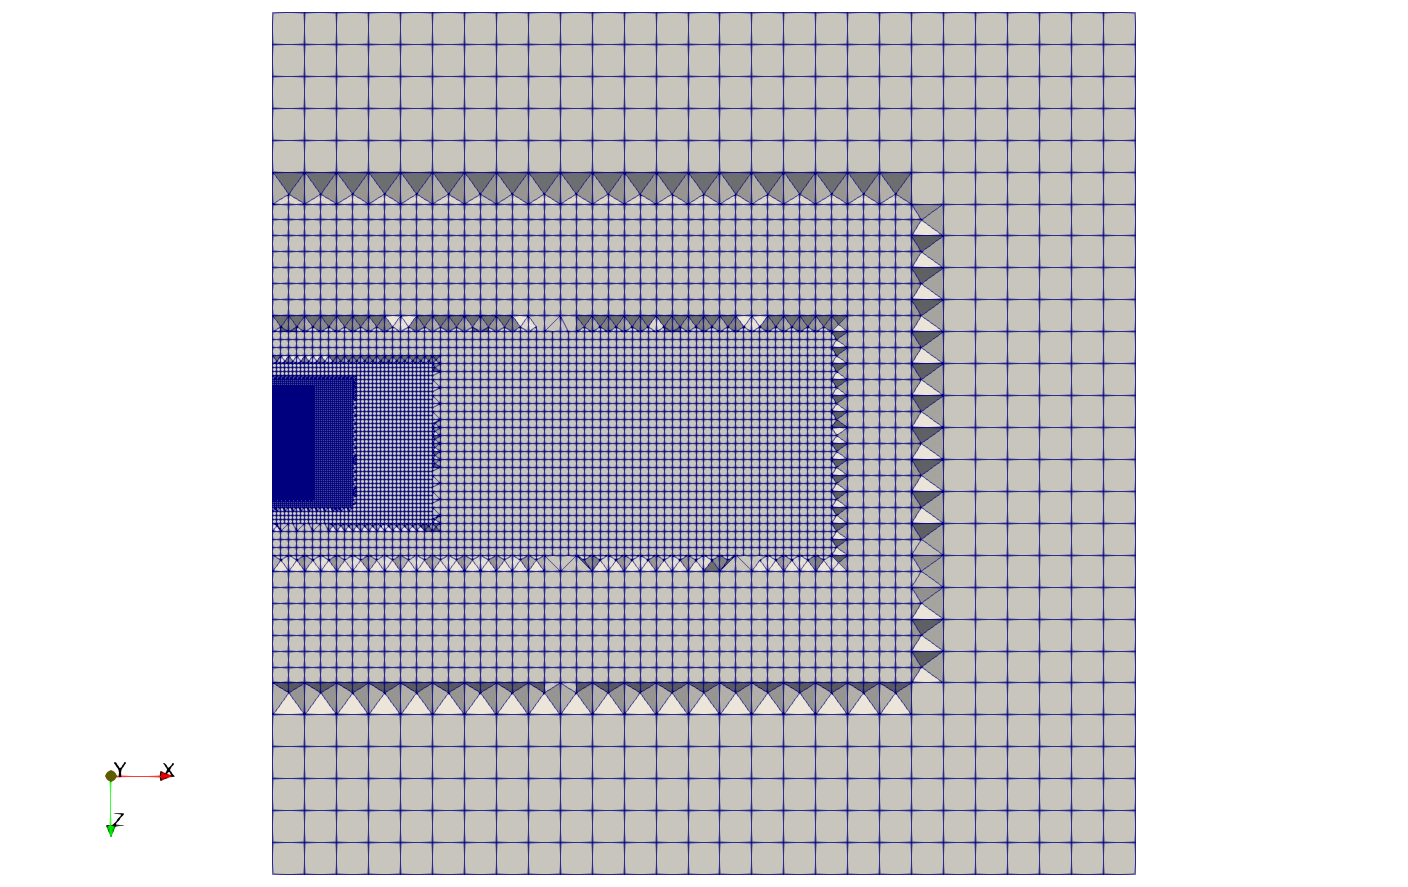
\includegraphics[width=\linewidth]{figs/MB18/side-view-mesh.png}
    \caption{Spatial domain discretisation.}
    \label{fig:enter-label}
\end{figure}

Coaxial-cylindrical refinement regions with respect to the injector nozzle centre (i.e., $(0 0 0)$), progressively finer towards the injection hole (nref=1):

\begin{center}
\begin{tabular}{llll}
\hline
Refinement level & Size [mm] & Radius [mm] & Height [mm] \\
\hline
0 & 4.0 & - & - \\
1 & 2.0 & 30 & 80 \\
2 & 1.0 & 15 & 70 \\
3 & 0.5 & 10 & 20 \\
4 & 0.25 & 8 & 10 \\
5 & 0.125 & 7 & 5 \\
\hline
\end{tabular}
\end{center}

Temporal resolution:
\begin{itemize}
    \item $\Delta t_{min} = 5\text{e-}7 \, [\mathrm{s}]$
    \item $\Delta t_{min} = 2\text{e-}7 \, [\mathrm{s}]$
\end{itemize}

\subsubsection*{Equation Discretisation}
\begin{itemize}
    \item Spatial derivatives and variables: See \texttt{system/fvSchemes}.
    \item Temporal derivatives and variables: See \texttt{system/fvSchemes}.
\end{itemize}

\subsubsection*{Numerical Boundary/Initial Conditions}
Refer to \texttt{0.orig}.

\subsubsection*{Pressure-Velocity Coupling Algorithm}
PISO.

\subsubsection*{Linear Solvers}
Refer to \texttt{system/fvSolution}.

\subsubsection*{Initialisation and Sampling}
No initialisation/averaging. Refer to \texttt{system/controlDict} for function objects being used.

\subsubsection*{Instructions to Run the Case}
The setup for nref=1 (baseline) is tested in OpenFOAM v2206. Execution is typically a call to Allrun script with required number of processors as argument. e.g., \texttt{./Allrun 16}.

\subsubsection*{Results}
%\paragraph{Liquid Penetration vs Time}
\begin{figure}[H]
    \centering
    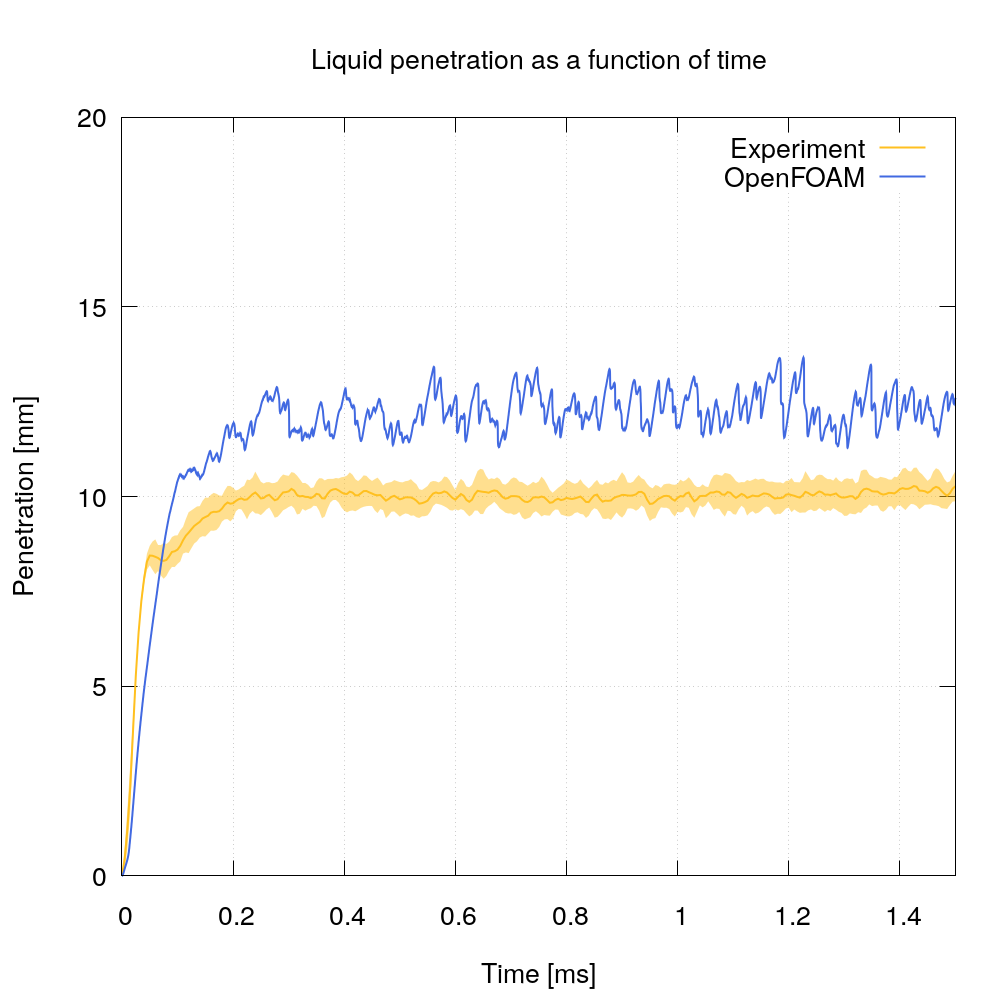
\includegraphics[width=0.9\linewidth]{figs/MB18/liquid_penetration.png}
    \caption{Liquid Penetration vs Time.}
    \label{fig:enter-label}
\end{figure}

%\paragraph{Vapor-phase Penetration vs Time}
\begin{figure}[H]
    \centering
    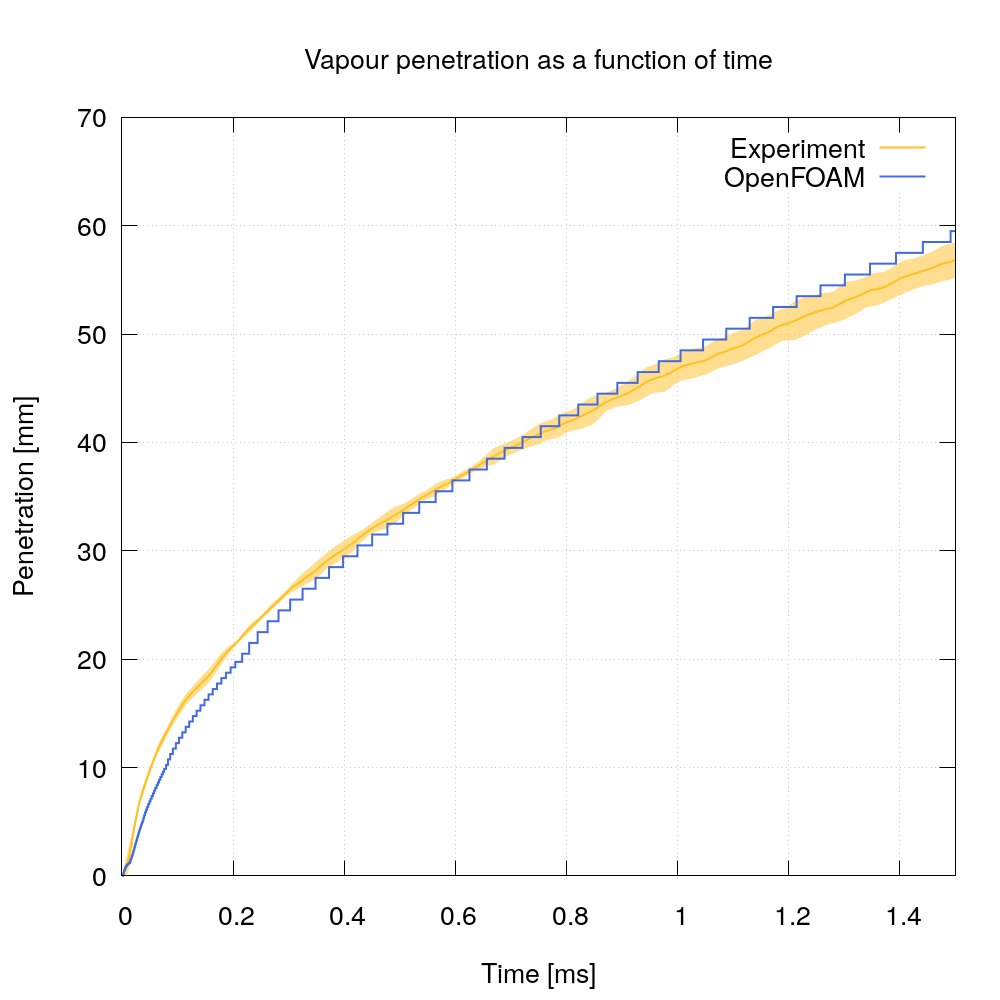
\includegraphics[width=0.9\linewidth]{figs/MB18/vapour_penetration.png}
    \caption{Vapor-phase Penetration vs Time.}
    \label{fig:enter-label}
\end{figure}

\subsubsection*{Bottlenecks}
The bottlenecks to be addressed in exaFOAM using the release code series OpenFOAM-vYYMM are:
\begin{itemize}
    \item Scalability of combined flow and Lagrangian OpenFOAM solvers
    \item Computational load between the continuum and discrete particle solvers (number of particles versus mesh count).
    \item Load-balancing and performance benchmarking as the Lagrangian particles transport in space.
\end{itemize}

\subsubsection*{Discussion}
\begin{itemize}
    \item The breakup model constant $B_1$ has a significant impact on the spray modeling, since it controls the diameter reduction of secondary droplets.
    \item In general, given a set of spray model parameters, the simulation results are not grid independent.
    \item Note that these gas velocities are small when compared to liquid (high-momentum) spray velocities (400 to 600 m/s) and therefore, have little effect on the sprays.
    \item The effect of URANS turbulence models on liquid penetration is not pronounced.
    \item Conversely, there is a significant discrepancy among the vapor penetration predictions over time.
\end{itemize}

%\subsection{DLR confined jet high pressure combustor}
%%%%%%%%%%%%%%%%%%%%%%%%%%%%%%%%%%%%%%%%%%%%%%%%%%%%%

The \href{https://develop.openfoam.com/exafoam/wp2-validation/-/tree/master/combustion/XiFoam/DLRCJH?ref_type=heads}{DLR confined jet high pressure combustor} stems from an experimental setup constructed by Severin at the Institute of Combustion Technology of the German Aerospace Center (abbreviated as DLR in German). The burner is based on the Recirculation-Stabilized Jet Flame (RSJF) concept, which is better known as FLOX. Initially developed for the industrial furnaces, this technology has a great potential in the application to the gas turbines. Compared to widespread swirl burners, RSJF combustors feature low NOx emissions, homogeneous temperature distribution, and operate with a wide range of fuels and loads. The main goal of the experimental work was to clarify how the recirculation contributes to the flow stabilization. Apart from the experiments, a number of numerical investigations with the same geometry was performed.

The considered combustor stems from an experimental setup constructed by Severin\footnote{\url{https://doi.org/10.18419/opus-9573}} at the Institute of Combustion Technology of the German Aerospace Center (DLR). The burner is based on the Recirculation-Stabilized Jet Flame (RSJF) concept, better known as FLOX. This technology, initially developed for industrial furnaces, has great potential in gas turbine applications. Compared to widespread swirl burners, RSJF combustors feature low NOx emissions, homogeneous temperature distribution, and operate with a wide range of fuels and loads. The main goal of the experimental work was to clarify how recirculation contributes to flow stabilization.

\begin{figure}[H]
    \centering
    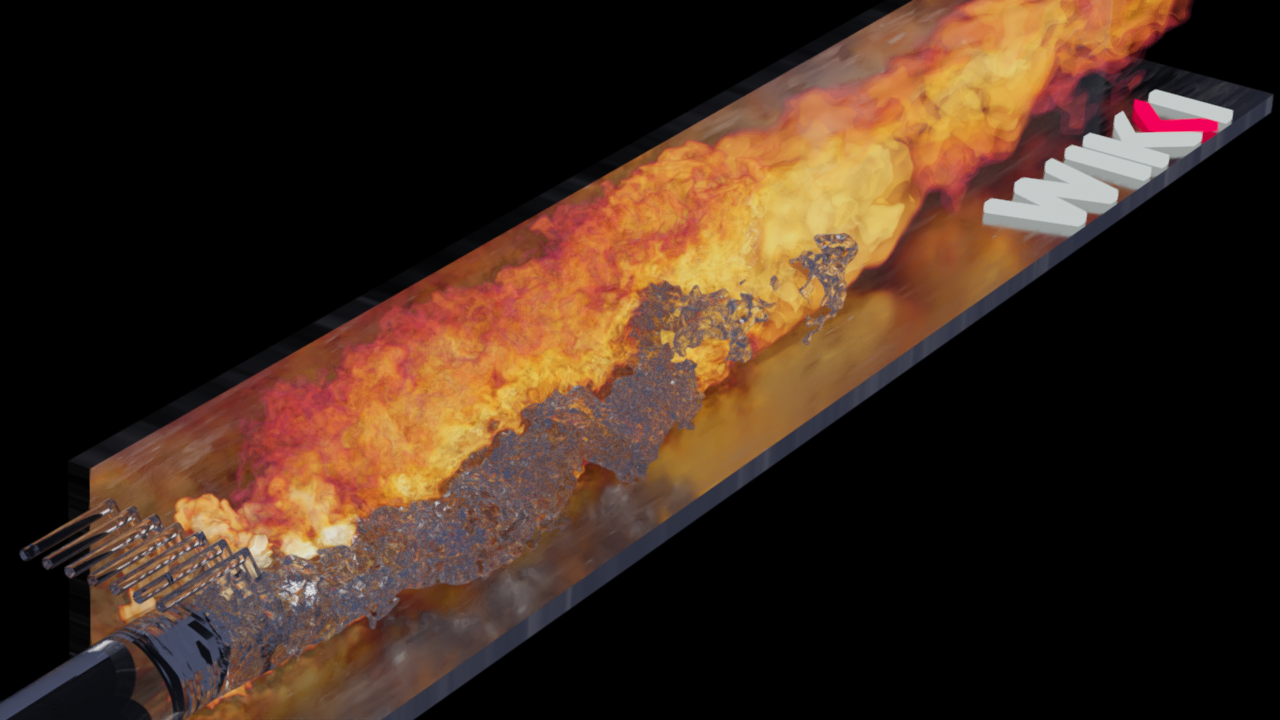
\includegraphics[width=\textwidth]{figs/DLRCJH/renderingDLRCJH.png}
    \caption{Rendering of the DLRCJH combustor flame with fuel.}
\end{figure}

\section*{Experimental Setup}
\begin{figure}[H]
    \centering
    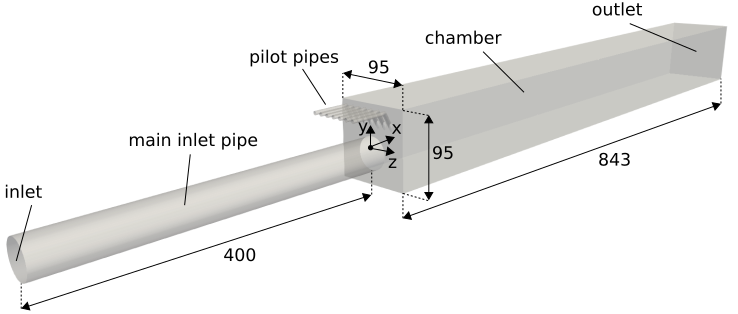
\includegraphics[width=\textwidth]{figs/DLRCJH/geometry_3D.png}
    \caption{Geometry of the combustor DLRCJH. Dimensions are in mm.}
\end{figure}

A typical RSJF combustor consists of several nozzles arranged in a ring around a central pilot swirl-burner. The test rig considered here represents a segment of such an RSJF combustor with a single nozzle\footnote{\url{https://doi.org/10.18419/opus-9573}}. It consists of a rectangular chamber with dimensions $95 \times 95 \times 843 \, \text{mm}^3$, a cylindrical inlet with a 40 mm diameter, a fuel injector placed 400 mm upstream of the chamber, and an outlet at the end of the chamber. The main inlet pipe axis is offset to the chamber centerline by 10 mm to allow for the recirculation zone to develop. The effect of the swirl-burner is simulated by seven pilot burners inclined to the main inlet axis and placed above the main inlet pipe. A premixed mixture of air and natural gas is injected through the main and pilot nozzles, where the overall mass flow of the pilots corresponds to 10\% of the main nozzle.

\section*{Measurements}
Severin\footnote{\url{https://doi.org/10.18419/opus-9573}} applied the following measurement techniques: OH*-chemiluminescence (identification of the flame position), Particle Image Velocimetry (PIV, flow speed determination), and Laser-Induced Fluorescence of the OH radical (LIF, temperature determination). The temperature and velocity fields from the middle slice (x-y plane) of the chamber were evaluated and are used here for validation.

\section*{Flow Parameters}
\begin{itemize}
    \item Reynolds number: 497,000;
    \item Average velocity at the main inlet: $\left| U_i \right| = 113 \, \text{m/s}$;
    \item Chamber pressure: 8 bar;
    \item Air-fuel ratio: 1.7;
    \item Inlet temperature of the mixture: $T_i = 725 \, K$;
    \item Adiabatic flame temperature: $1950 \, K$.
\end{itemize}

\section*{Numerical Setup}

\subsection*{Geometry}
The geometry parameters shown in the table below are taken from Severin\footnote{\url{https://doi.org/10.18419/opus-9573}}.

\begin{table}[H]
    \centering
    \begin{tabular}{ll}
        \hline
        Dimension & Description \\ \hline
        $d_i = 40 \, \text{mm}$ & Inlet nozzle diameter \\
        $y_i = -10 \, \text{mm}$ & Vertical offset of the nozzle mounting point \\
        $a = 95 \, \text{mm}$ & Lateral, top, and bottom wall width of the chamber \\
        $l = 843 \, \text{mm}$ & Chamber length \\
        $x_{inj} = -400 \, \text{mm}$ & Location of the fuel injection \\
        $d_o = 58.8 \, \text{mm}$ & Outlet nozzle diameter \\
        $d_p = 4.7 \, \text{mm}$ & Pilot nozzle diameter \\
        $\alpha = 60^\circ$ & Inclination angle of the pilot nozzles to the inlet nozzle axis \\
        $\Delta z_p = 10 \, \text{mm}$ & Distance between neighboring pilot nozzles \\
        $y_p = 25 \, \text{mm}$ & Vertical offset of the pilot nozzles mounts \\ \hline
    \end{tabular}
\end{table}

\subsection*{Initialization}
The flow is initialized either by means of *setFields* or *mapFieldsPar*. The former is used when no field data from a run of lower resolution is available. Utility *mapFieldsPar* is used for propagating the developed flow from cases with lower mesh resolution to higher ones, lowering the cost-to-solution.

\subsection*{Models}
\begin{itemize}
    \item Solver: **XiFoam** is used as the top-level solver. It handles unsteady compressible flow, incorporates combustion-relevant models, and is controlled by a PIMPLE loop allowing CFL numbers higher than 1.
    \item Turbulence: LES kinetic energy equation model (*kEqn*) with van Driest damping function for near-wall treatment.
    \item Combustion: The fuel mixture is inhomogeneous since the main and pilot nozzles are operated with different air-to-fuel ratios. The laminar flame speed $S_u$ is assumed to be unstrained, and a transport equation is solved for the flame wrinkling $\Xi$.
\end{itemize}

\subsection*{Numerics}
LES modeling relies on high accuracy discretization, utilizing higher-order schemes like *linear*, *limitedLinear*, and *limitedLinear01*. For velocity convection, *filteredLinear* is used. Temporal discretization uses a blending between Euler and Crank-Nicolson with a ratio of 30:70 (*crankNicolson 0.7*). Linear solvers are based on the conjugate gradients method. The PIMPLE loop has 2 outer and 1 inner corrections with 0 non-orthogonal corrections. Utility *renumberMesh* is used to reduce matrix bandwidth and accelerate linear solver execution.

\subsection*{Surface Mesh}
Surface mesh is created using FreeCAD 0.20\footnote{\url{https://wiki.freecad.org/Release_notes_0.20}}.

\subsection*{Mesh}
Meshing is accomplished with *snappyHexMesh (sHM)*. Four surface meshes are provided:
- An .obj file with the complete geometry with regions corresponding to boundaries.
- An .stl file with the complete geometry without regions.
- Two additional .stl files with surface meshes of the inlet pipe and pilots.

Four meshes with resolutions of 3M, 24M, 189M, and 489M cells have been produced successively.

\section*{Boundary Conditions}
\begin{table}[H]
    \centering
    \begin{tabular}{lllll}
        \hline
        Quantity & Main Inlet & Pilot Inlet & Walls & Outlet \\ \hline
        $\alpha_t$ & zG & zG & wF & c \\
        $b$ & fV 1 & fV 1 & zG & iO 0 \\
        $f_t$ & fV 0.03344 & fV 0.06084 & zG & iO 0.03344 \\
        $k$ & fV $1e-5$ & fV $1e-5$ & wF & iO $1e-5$ \\
        $\nu_t$ & c & c & zG & c \\
        $p$ & zG & zG & zG & wT $8e5$ 5 \\
        $S_u$ & c & c & zG & c \\
        $T$ & fV 725 & fV 633 & CF: fV 600; CL: fV 800; other: zG & iO 1000 \\
        $T_u$ & fV 725 & fV 633 & CF: fV 600; CL: fV 800; other: zG & iO 1000 \\
        $U$ & fRIV 0.5563 & fRIV 0.0558 & fV $(0, 0, 0)$ & iO $(0, 0, 0)$ \\
        $\Xi$ & fV 1 & fV 1 & zG & iO 20 \\ \hline
    \end{tabular}
\end{table}

Abbreviations:
\begin{itemize}
    \item c: calculated BC;
    \item CF: Chamber Front (baseplate);
    \item CL: Chamber Lateral walls;
    \item fRIV *massFlowRate*: flowRateInletVelocity BC;
    \item fV *value*: fixedValue BC;
    \item iO *inletValue*: inletOutlet BC;
    \item wF: wallFunction BC;
    \item wT *fieldInf* *lInf*: waveTransmissive BC;
    \item zG: zeroGradient BC.
\end{itemize}

\section*{Validation}
Validation was performed with results from Severin\footnote{\url{https://doi.org/10.18419/opus-9573}} using the case with 24 million cells. Temperature and velocity profiles were averaged over 0.05 seconds of physical time.

\begin{figure}[h]
    \centering
    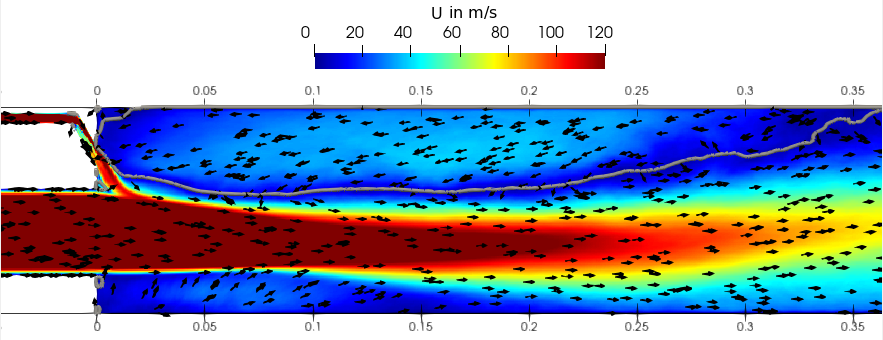
\includegraphics[width=0.8\textwidth]{figs/DLRCJH/7608d6e2c381894c3303bca616371060.png}
    \caption{Velocity comparison: Computation vs. Experiment.}
\end{figure}

\section*{Grand Challenge}
\begin{itemize}
    \item Known to run with OpenFOAM-v2106, -v2112, -v2306 compiled with double precision.
    \item Three cases are provided: 3M, 24M, and 489M.
    \item Two setups for each mesh size are provided: *fixedTol* and *fixedIter*.
\end{itemize}

\section*{Known Issues}
\begin{itemize}
    \item During meshing, a bug related to FMA instructions has been encountered.
    \item Utility *mapFieldsPar* failed to map from 189M to 489M while using collated fileHandler.
    \item Provided coded function object *FOwallClockTimeStatistics* may cause issues during startup.
\end{itemize}

\section*{Benchmark Results}
Two supercomputers were used for benchmarking: HAWK and LUMI.

\subsection*{Strong Scaling}
Normalized time to solution is calculated as $T_i^* = t_i N_c / N_e$, where $t_i$ is the time per iteration, $N_c$ is the number of cores, and $N_e$ is the number of cells.

\subsubsection*{3M Case}
\begin{figure}[h]
    \centering
%    \includegraphics[width=0.8\textwidth]{figures/speedup_3M.png}
    \caption{Speedup for the 3M case.}
\end{figure}

\subsubsection*{24M Case}
\begin{figure}[h]
    \centering
%    \includegraphics[width=0.8\textwidth]{figures/speedup_24M.png}
    \caption{Speedup for the 24M case.}
\end{figure}

\subsubsection*{489M Case}
\begin{figure}[h]
    \centering
%    \includegraphics[width=0.8\textwidth]{figures/speedup_489M_largeRunsOnly.png}
    \caption{Speedup for the 489M case.}
\end{figure}

\subsection*{Weak Scaling}
Weak scaling benchmarks were performed for loads of 60K, 30K, 15K, and 7.5K cells per core.

\section*{Coherent File Format}
The coherent format addresses major IO bottlenecks, resulting in significant improvements:
- Case decomposition: up to 60 times lower time-to-solution.
- Overall pre- and post-processing: 31 times lower cost-to-solution.
- Solver execution: 30 times lower time-to-solution.
%\subsection{DLR Jet-in-Hot-Coflow Burner}
%%%%%%%%%%%%%%%%%%%%%%%%%%%%%%%%%%%%%%%%%
For \href{https://develop.openfoam.com/committees/hpc/-/tree/develop/combustion/reactingFoam/LES/DLRJHC}{DLR Jet-in-Hot-Coflow Burner} testcase, 
the solution of stiff ordinary differential equations (ODEs) systems is of key importance in advanced multiphysics CFD simulations; in reactive flow simulations the fluid transport is coupled to the solution of finite-rate chemistry problems. In these scenarios, the computational effort connected to the integration of the detailed chemical kinetics ODEs systems largely contributes to limit the solver speed. A possible solution to overcome this inconvenience consists of integrating the chemical ODEs systems via an adaptive multi-block explicit solver running on a Graphical Processing Unit (GPU). The idea is to dynamically redistribute the ODE system over the resources available from the GPU architecture, while the Navier-Stokes equations are solved by a multi-core CPU algorithm. The hybrid CPU/GPU solver is expected to provide a significant speed-up in reactive calculations. The performance gain is expected to increase with large-scale mechanisms, that are characterized by large workloads.

\section*{Configuration}
\begin{figure}[h]
    \centering
%    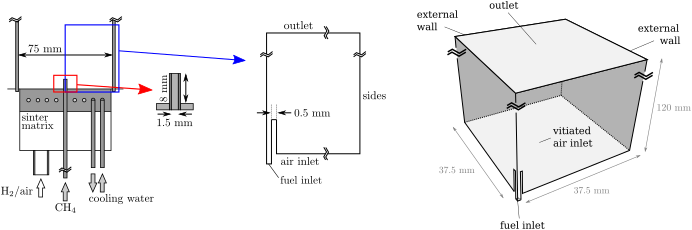
\includegraphics[width=0.6\textwidth]{figures/DLRJHC-geom.png}
    \caption{The three-dimensional geometry is based on the information available from the literature. Simplifications are introduced to account for one quarter of the entire top construction due symmetry planes.}
\end{figure}

Figure 1 (left) presents the entire structure; detailed information is reported in the literature\footnote{\url{https://doi.org/10.1080/13647830.2020.1715993}}. A pre-chamber exists below a top vessel. The top vessel is considered in the current analysis (see Fig. 2); the pre-chamber is neglected. The top of the considered chamber is open. A jet of fuel is introduced in the vessel; the region is initially filled with vitiated air coming from a preliminary combustion process between air and $H_2$ which takes place in the pre-chamber. The vitiated air is accounted as a homogeneous mixture because of the perfect mixing occurring in the pre-chamber. In the top vessel, the hot vitiated air reacts with the injected methane and generates a steady lift flame. Experiments are publicly available from the DLR Institute of Combustion Technology. 

The $L \times W \times H$ rectangular-shaped region is three-dimensional. Due to the introduced simplification, a quarter of the domain can be considered; symmetry planes are identified on two of the resulting sides. A small centered nozzle injects the fuel, while air with lean premixed hydrogen combustion products is introduced at the bottom of the mesh in the surrounding region. The walls of the fuel injector have thickness $t_w = 0.5 \, \text{mm}$. The injector diameter is $d = 2 \, \text{mm}$. The chamber has real dimensions $L \times W = 80 \, \text{mm} \times 80 \, \text{mm}$. The top is used as outlet for combustion products, thus an inlet-outlet boundary condition is applied. The temperature of the jets is $T_f = 600 \, K$ and $T_{air} = 1490 \, K$; the internal field temperature is $T_{if} = 600 \, K$. Atmospheric pressure is imposed initially. Air is used as oxidizer, but it contains a mixture of hydrogen combustion products: the mixture is composed by 72\% of $N_2$, 10\% of $O_2$, 0.2\% of $OH$, and finally 18\% of $H_2O$. The Courant number is preserved low.

\section*{Measurements}
Experiments are available from the literature for code validation\footnote{\url{https://doi.org/10.1080/13647830.2020.1715993}}.

\section*{Flow Parameters}
\begin{itemize}
    \item The fuel jet enters with high velocity: $\left| U \right| = 163.18 \, \text{m/s}$;
    \item The surrounding air (vitiated) at high temperature: $T_{air} = 1490 \, K$;
    \item Premixed lean hydrogen-air mixture from the below chamber;
    \item Premixed lean hydrogen-air mixture assumed homogeneous and reacting with methane (in top channel).
\end{itemize}

\section*{Numerical Setup}
The numerical setup is based on the DLR tutorial available in OpenFOAM-v2206. A detailed description is available on the OpenFOAM wiki\footnote{\url{https://openfoamwiki.net/index.php/Main_Page}}. The changes that allow the treatment of the considered case via GPU chemistry model are proposed subsequent sections, and include the modification of the \textit{chemistryProperties} and \textit{controlDict} files, contained in the \textit{constant} and \textit{system} folder respectively. They are consistent with the modifications proposed for the microbenchmark test case (counterFlowFlame2D). No changes are required to the numerical schemes, or to the settings of the numerical solvers. Mesh- and BC-related modifications to the problem are made to adequately treat the DLR-JHC test case.

\subsection*{Geometry and Mesh}
The problem is three-dimensional. The $L \times W \times H$ rectangular-shaped region has internal dimensions $75 \, \text{mm} \times 75 \, \text{mm} \times 120 \, \text{mm}$. The problem is reduced by considering one-quarter of the chamber; for this reason, while two external boundaries are set as walls, the remaining two are marked as symmetry planes. A single round injector of fuel is present at the center of the burner in the full construction; because of the simplification, the problem is reduced to the investigation of a quarter of the injector. Conversely to a similar tutorial available in OpenFOAM-v2206\footnote{\url{https://openfoamwiki.net/index.php/Main_Page}} (which is anyway used as starting point for the current configuration), the domain cannot be represented by means of a wedge structure: the surrounding casing (which defines the burner geometry) has a squared footprint. The mesh is generated via the \textit{blockMesh} meshing utility.

\subsection*{Models}
\begin{itemize}
    \item Solver: \textbf{reactingFoam} is used as the top-level solver.
    \item Turbulence: the problem is turbulent, hence a LES turbulence model is used.
    \item Combustion: a Partially Stirred Reactor (PaSR) combustion model is adopted.
\end{itemize}

\subsection*{Numerics}
First order, bounded, implicit time scheme; first/second order unbounded limitedLinear divergence schemes; the PIMPLE loop has 1 outer and 2 inner corrections with 0 non-orthogonal corrections. Momentum predictor is active. The fluid dynamic time step interval is initially set to $1e-6$ with an endtime of $1e-3$; the time advancement is regulated via the settings of a maxDeltaT and a maximum acceptable Courant number.

\subsection*{Boundary Conditions}
\begin{table}[H]
    \centering
    \begin{tabular}{lll}
        \hline
        Variable & Description & Units \\ \hline
        $U$ & Axial velocity & $m/s$ \\
        $p$ & Pressure & $Pa$ \\
        $T$ & Temperature & $K$ \\
        $Y_i$ & Mass fraction of the $i$-th chemical specie & - \\
        $k$ & Turbulent kinetic energy & $m^2/s^2$ \\
        $\nu_t$ & Turbulent viscosity & $m^2/s$ \\
        $\alpha_t$ & Turbulent thermal diffusivity & $kg/(m.s)$ \\ \hline
    \end{tabular}
\end{table}

\subsubsection*{Internal Field}
Pressure $p = 1e5 \, Pa$; temperature $T_{air} = 1490 \, K$; The methane concentration is 0. $Y_{N_2} = 0.7554$, $Y_{O_2} = 0.1229$, $Y_{OH} = 0.001$, and finally $Y_{H_2O} = 0.1207$. The internal field of the velocity is set to $\left| U \right| = 4.1$ along the chamber elongation (toward the outlet).

\subsubsection*{Fuel Inlet}
\begin{table}[H]
    \centering
    \begin{tabular}{lll}
        \hline
        Variable & Type & Value \\ \hline
        $U$ & fixedValue & 163.18 \\
        $p$ & zeroGradient & - \\
        $T$ & fixedValue & 600 \\
        $\alpha_t$ & calculated & 0 \\
        $\nu_t$ & calculated & 0 \\
        $k$ & fixedValue & 0.375 \\
        $Y_{O_2}$ & fixedValue & 0 \\
        $Y_{N_2}$ & fixedValue & 0 \\
        $Y_{OH}$ & fixedValue & 0 \\
        $Y_{H_2O}$ & fixedValue & 0 \\
        $Y_{CH_4}$ & fixedValue & 1 \\ \hline
    \end{tabular}
\end{table}

For $U$, the value comes from the imposition of a mass flow rate, considering a density value $\rho_{f} = 0.71682 \, kg/m^3$.

\subsubsection*{Air Inlet}
\begin{table}[H]
    \centering
    \begin{tabular}{lll}
        \hline
        Variable & Type & Value \\ \hline
        $U$ & fixedValue & 4.1 \\
        $p$ & zeroGradient & - \\
        $T$ & fixedValue & 1490 \\
        $\alpha_t$ & calculated & 0 \\
        $\nu_t$ & calculated & 0 \\
        $k$ & turbulentIntensityKineticEnergyInlet & 0.02 \\
        $Y_{O_2}$ & fixedValue & 0.1207 \\
        $Y_{N_2}$ & fixedValue & 0.7554 \\
        $Y_{OH}$ & fixedValue & 0.001 \\
        $Y_{H_2O}$ & fixedValue & 0.1229 \\
        $Y_{CH_4}$ & fixedValue & 0 \\ \hline
    \end{tabular}
\end{table}

\subsubsection*{Outlet}
\begin{table}[H]
    \centering
    \begin{tabular}{lll}
        \hline
        Variable & Type & Value \\ \hline
        $U$ & pressureInletOutletVelocity & internalField \\
        $p$ & totalPressure & internalField \\
        $T$ & inletOutlet & internalField \\
        $\alpha_t$ & calculated & internalField \\
        $\nu_t$ & calculated & internalField \\
        $k$ & inletOutlet & internalField \\
        $Y_{O_2}$ & inletOutlet & internalField \\
        $Y_{N_2}$ & inletOutlet & internalField \\
        $Y_{OH}$ & inletOutlet & internalField \\
        $Y_{H_2O}$ & inletOutlet & internalField \\
        $Y_{CH_4}$ & inletOutlet & internalField \\ \hline
    \end{tabular}
\end{table}

\section*{Validation}
The GRI-Mech 3.0 chemical chain is added to the \textit{constant} folder. A preliminary set of results is available in the \textit{validation} state. The results contained in the postProcessing folder must be consistent with those available in the \textit{validation/CPU} folder, obtained at endTime (hot simulation). The solutions are extracted along multiple axial lines across the real three-dimensional domain.

\begin{figure}[h]
    \centering
%    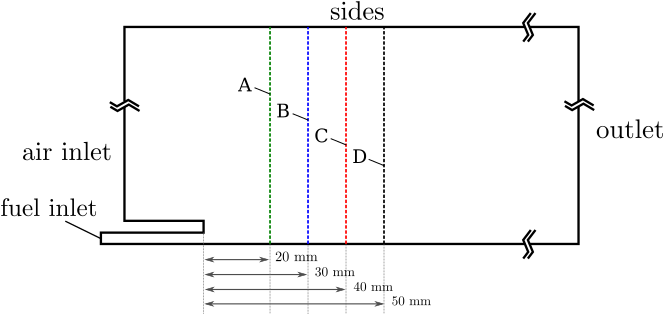
\includegraphics[width=0.8\textwidth]{figures/DLRJHC-lines.png}
    \caption{Axial lines in the geometry.}
\end{figure}

The code validation is performed by comparing the results produced by the developed run against those available in the literature.

\section*{Benchmark}
\begin{itemize}
    \item Known to run with OpenFOAM-v2206;
    \item A single folder case is provided;
    \item Multiple tests can be performed by varying the number of cells;
    \item The time taken to perform code validation and complete the simulation with the proposed setup depends on the computational hardware and the multi-core availability;
    \item Automatic light post processing for code validation via \textit{gnuplot} eases code development and debug;
    \item Heterogeneous CPU/GPU solution can be obtained by following the instruction provided for the microbenchmark counterFlowFlame2D.
\end{itemize}

\section{Resources}
%%%%%%%%%%%%%%%%%%%
\begin{itemize}
    \item \url{https://web.stanford.edu/group/haiwanglab/HyChem/pages/download.html}
    \item \url{https://dustsafetyscience.com/chemkin-openfoam-converter}
    \item \url{https://www.cerfacs.fr/cantera/mechanisms/meth.php#1S}
    \item \url{https://ctrfl.princeton.edu/databases}
    \item \url{https://rmg.mit.edu}
    \item \url{https://cantera.org/index.html}
    \item \url{https://github.com/AndyShor/RD_107}
    \item \url{https://janaf.nist.gov}
    \item \url{https://www.youtube.com/watch?v=vhQHClufqWY} %  CFD Simulation of a Combustion Chamber: Combustion Model with NOx and Soot in Ansys Fluent 
    \item \url{https://www.youtube.com/watch?v=dUme0MUoqbk} %  Complete OpenFOAM tutorial - from geometry creation to postprocessing 
    \item \href{https://www.youtube.com/watch?v=wmWQBOAOtLc}{ANSYS Fluent: Non-premixed Combustion using the Steady Flamelet Model}
    \item \href{https://www.youtube.com/watch?v=PTdZyy6kxI0}{ANSYS Fluent: Diffusion Controlled Reacting Flow in a Can Combustor}
    \item \href{https://ansyshelp.ansys.com/public/account/secured?returnurl=/Views/Secured/prod_page.html?pn=Fluent}{Fluent tutorials}
\end{itemize}

\section{Conclusion}
%%%%%%%%%%%%%%%%%%%%

A number of critical points for this numerical simulation's campaign have been highlighted, such as:
%
\begin{itemize}
    \item Increase of the computational cost with detailed chemistry.
    \item Choice of the appropriate turbulence-chemistry interaction models (e.g., EDC, PDF).
    \item Validation of the results against experimental data or benchmark cases.
\end{itemize}

%%%%%%%%%%%%%%%%%%%%%%%%%%%%%%%%%%%%%%%%%%%%%%%%%%%%%%%%%%%%%%%%%%%%%%%%%%%%%%%%
\vspace{\fill}
\begin{center}
    \hspace*{-9.0cm} \LARGE \textbf{Lorenzo Campoli} \\
    \hspace*{-9.0cm}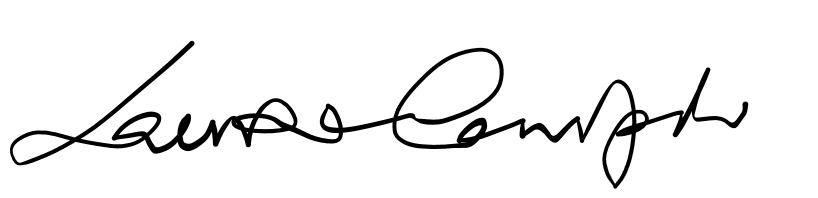
\includegraphics[width=0.45\textwidth]{signature.png}
\end{center}
%%%%%%%%%%%%%%%%%%%%%%%%%%%%%%%%%%%%%%%%%%%%%%%%%%%%%%%%%%%%%%%%%%%%%%%%%%%%%%%%

\vspace*{-1.0cm}

\textbf{Senior Systems Modelling Engineer}

\textbf{Gilmour Space Technologies}

\textbf{lorenzo.campoli@gspace.com}%\\

%\newpage

%\nocite{*}
\bibliography{refs}
\bibliographystyle{plain}

\end{document}